%===========================================================
%     		Expanded Main document for my PhD. Thesis.
%
% 			ÁNGEL MIGUEL GARCÍA VICO (agvico@ujaen.es)
%			
%			To build it you need to run XeLaTeX and Biber in this order:
% 			 - xelatex
%			 - biber
%			 - xelatex (x2)
%
%  I think it will work also with pdflatex, but I didn't try it.
%===========================================================

\documentclass[c5paper,10pt,twoside]{book}	   	% Book format in C5 paper size (6.5x9")

\usepackage[dvipsnames]{xcolor}		% For the "Midnight Blue" color
\usepackage{varioref}		% Smart referencing
\usepackage[hidelinks,hypertexnames=false]{hyperref}  % Hyperlinks and URLs
\usepackage[numbered]{bookmark}  % For PDF bookmarks
\usepackage[utf8]{inputenc}		 % For writing tildes (useful in spanish)
\usepackage{titlesec}			 % Customs chapter and section headings
\usepackage{graphicx,fancyhdr,amsmath,amssymb,mathtools,algorithm,algorithmicx,algpseudocode,multirow,booktabs,caption,tabulary,tabularx,tikz}  % many useful packages
\usetikzlibrary{shapes,arrows,fit,positioning,backgrounds}
\usepackage[english,spanish]{cleveref}  % Smart references
\crefname{table}{\spanishtablename}{\spanishtablename}  % Translations to spanish
\usepackage[Sonny]{fncychap}  % Base header & footer
\usepackage[british, spanish, es-tabla]{babel}  % Language package
\usepackage{csquotes}  % quotes according to gramitical rules of the language set
\usepackage{datetime}  % to get the \today day.
\usepackage{microtype} % Microtyping help 
\usepackage{libertine, eulervm} 	% text & math fonts respectively
\usepackage[printonlyused]{acronym} % For the acronyms.
\usepackage[backend=biber,style=ieee,natbib=true,maxnames=10]{biblatex}  % Bibliography
\addbibresource{./referencias.bib}
\DeclareFieldFormat*{citetitle}{#1}

\definecolor{azul}{rgb}{0,33,113}
\usepackage[toc,page]{appendix}

\usepackage[top=0.5in, 
			outer=0.5in, 
			bottom=0.5in,
			inner=0.75in,
			headsep=10pt,
			c5paper]{geometry}   % Margin and geometry settings
			
\usepackage[defaultlines=3,all]{nowidow}   % Widow and club management
\usepackage[caption=false]{subfig}    % Subfigures 
\usepackage{usebib}		 % full cites
\usepackage{pdfpages} \urlstyle{same}	% add pdfs 

\usepackage[width=16.2truecm, height=22.9truecm,frame,axes, pdftex,center]{crop}

\newcommand{\chapnumfont}{\usefont{T1}{pnc}{b}{n}\fontsize{80}{80}\selectfont }
\colorlet{chapnumcol}{MidnightBlue}  

\titleformat{\chapter}[display]
{\filleft\bfseries}
{\filleft\chapnumfont\textcolor{chapnumcol}{\thechapter}}
{-24pt}
{\Huge}

\titleformat{\section}
[block]
{\bfseries\Large}
{\llap{\makebox[0.5in][l]{\color{MidnightBlue}\thesection.}}}
{0pt}
{}

\titleformat{\subsection}
[block]
{\bfseries\large}
{\llap{\makebox[0.5in][l]{\color{MidnightBlue}\thesubsection.}}}
{0pt}
{}



\newdateformat{monthyeardate}{\monthname[\THEMONTH] de \THEYEAR}

\captionsetup[table]{skip=10pt} 
\setcounter{secnumdepth}{3}
\setcounter{tocdepth}{3}
\floatname{algorithm}{Algoritmo} 
\addto\captionsspanish{\renewcommand\appendixpagename{Apéndices}}

\newcounter{incluirPDF}
\setcounter{incluirPDF}{0}

\newcommand*\Let[2]{\State #1 $\gets$ #2}
\newcommand{\doi}[1]{\href{https://doi.org/#1}{#1}}
\newcommand{\incluirPaper}[2]{
	\ifnum\value{incluirPDF}>0 {
		
		\clearpage
		
		\includepdf[pages=#1]{#2}
		
		\cleardoublepage
		
	}\fi
}
\newcommand{\doubleline}{\midrule \midrule}


\fancyfoot{}
\fancyfoot[CE,CO]{\thepage}

\makeatletter
\let\ps@plain\ps@empty
\makeatother
\renewcommand{\footrulewidth}{0.0pt} 



\def\autor{Ángel Miguel García Vico}
\def\titulo{Modelos descriptivos basados en aprendizaje supervisado para el tratamiento de big data y flujos continuos de datos}
\def\universidad{Universidad de Jaén}
\def\centro{Escuela Politécnica Superior de Jaén}
\def\tutorUno{Pedro González García}
\def\dptoUno{Departamento de Informática}
\def\tutorDos{Cristóbal José Carmona del Jesus}
\def\dptoDos{Departamento de Informática}
\def\estudios{Departamento de Informática \\ \bigskip Universidad de Jaén}
\def\tipoTrabajo{Tesis Doctoral \\ con Mención en \sc doctorado internacional}
\def\localidad{Jaén}

\DeclareBibliographyCategory{important}
\AtEveryBibitem{\ifcategory{important}{\color{MidnightBlue}}{}}

\addtocategory{important}{Lgpc16,
Gcgcd16,
Gcmgj18,
Gcgd18,
Gcgd19,
Lcgjv19,
Gcgd19a,
Gmacd16,
Ggdc17,
Ggcd17,
Cggd19,
Cpggd15,
Gcgcj15,
604,
Gcd17,
Gcgd18b,
275
}


\hyphenation{e-mer-gen-tes }


\begin{document}

\clearpage{}



\pagestyle{empty}


\newgeometry{hmarginratio=3:2} 

\begin{titlepage}
	\begin{center}
		\Huge{\textsc{\universidad}}
		
		\Large{\textit{\centro}}
		
		\bigskip
		\bigskip
		\bigskip
		\bigskip
		
		\begin{tabulary}{\textwidth}{C}
			\doubleline
			\Large{\textsc{\textbf{\titulo.}}} \\
			\doubleline \\ \\
			\textbf{\Large{Memoria presentada por}} \\
			\LARGE{\textsc{\autor}}
			\\
			\\
			\\
			\\
			\Large{Para optar al Grado de Doctor en Informática \linebreak con \sc mención internacional}
		\end{tabulary}
	
	\vspace{\fill}
	
	\large{Fdo.: \sl{\autor.}}
		
	\end{center}
\end{titlepage}







\cleardoublepage

\mbox{}
\vfill
\begin{figure*}[!hbtp]
	\centering
	\subfloat{
		
\includegraphics[width=0.5\linewidth,keepaspectratio]{./Figures/logoMICINN}
	}
	\subfloat{
		
\includegraphics[width=0.41\linewidth,keepaspectratio]{./Figures/logoMINECO.eps}
	}
\end{figure*}

Tesis Doctoral parcialmente subvencionada por el Ministerio de Ciencia, Innovación y Universidades a través de la convocatoria \textit{Ayudas para Contratos Predoctorales 2016} (referencia BES-2016-077738), y parcialmente subvencionada por el Ministerio de Economía y Empresa bajo el proyecto con referencia  TIN2015-68454-R, Fondos FEDER.


\cleardoublepage




\textbf{D. \tutorUno} y \textbf{D. \tutorDos}, Profesores Titulares de Universidad del \dptoUno~de la \universidad

\bigskip
\bigskip

\textsc{informan}

\bigskip
\bigskip

Que la memoria titulada ``\textit{\titulo}'' ha sido realizada por \textbf{D. \autor} bajo su supervisión dentro del Programa de Doctorado en Tecnologías de la Información y la Comunicación para optar al grado de doctor. 

\bigskip
Para su evaluación, esta memoria se presenta como un conjunto de trabajos publicados, acogiéndose y ajustándose a lo establecido en el punto 2 del artículo 25 del \textit{Reglamento de los Estudios de Doctorado de la \universidad}, aprobado en febrero de 2012 y modificado en febrero de 2019.


\vspace{5mm}

\begin{flushright}
	Jaén, a 26 de febrero de 2020
\end{flushright}

\vspace{\fill}

\begin{center}
	\begin{tabular}{cc}
		Fdo. \tutorUno & ~~~~~Fdo. \tutorDos \\
		Tutor y Director de la Tesis & ~~~~~Director de la Tesis
	\end{tabular}
\end{center}


\cleardoublepage
\begin{flushright}
	\vspace*{\stretch{1}}
	\textit{A mis padres, por su enorme esfuerzo y sacrificio.\\Os quiero.}
	\par \vspace*{\stretch{3}}
\end{flushright}
%
\clearpage{} \cleardoublepage


\cleardoublepage
\clearpage{}\chapter*{Agradecimientos}



``Bienvenido a la montaña rusa de la investigación''. Estas fueron las primeras palabras de Cristóbal cuando empecé a investigar. No le faltaba razón. Tras estos años, el camino no ha sido fácil y ha estado lleno de obstáculos: jornadas de trabajo que se alargan hasta el infinito, experimentaciones fallidas, rechazo de artículos, etc. Sin embargo, tras haber llegado hasta aquí, y con cierta perspectiva, tengo que decir que ha merecido la pena. Por esta razón, me gustaría dedicarles unas líneas a las personas que me han apoyado y me han permitido llegar hasta este punto, pues sin ellos hubiera sido imposible.

En primer lugar, a mis padres. A pesar de no tener ningún tipo de estudios y de que encuentren muy complejo el mundo académico, me han enseñado una filosofía de vida y una forma de ser que no se aprende en la escuela. Ese esfuerzo que habéis realizado para que dé siempre lo máximo de mí ha permitido que hoy sea quien soy y esté donde estoy. Hoy, os podéis sentir orgullosos del fruto que habéis ido cultivando durante tanto tiempo.

En segundo lugar a mis directores de tesis. Sin Cristóbal y sin Pedro este trabajo no hubiera sido posible. Sus comentarios, ideas y apoyo han permitido que se desarrolle un trabajo de excepcional calidad. Todo ello acompañado de la capacidad necesaria para hacerme crecer como investigador, la cual me ha permitido afrontar con cada vez mayor capacidad la difícil tarea de investigar. 

También agradecer al grupo de investigación SiMiDat por hacerme sentir un compañero más de trabajo y por el todo el apoyo aportado. Me gustaría agradecer en especial a María José. Sin ella no hubiera empezado a investigar y no hubiera estado aquí. Por esto, y por todo el apoyo y oportunidades que me has dado desde mis inicios te estoy enormemente agradecido.

Gracias a Milton García-Borroto y a Diana Martín por el apoyo proporcionado a la hora de realizar la revisión de la literatura sobre EPM. Sin vosotros el trabajo realizado hubiera sido extremadamente complejo. También agradecer a David Elizondo por la oportunidad de realizar una estancia de investigación en DeMontfort University, Leicester, de donde ha salido un gran trabajo, junto a una gran experiencia vital. \textit{Thanks to Huseyin Seker for the invitation to the Northumbria University in order to perform a research stay. It was a great experience at Newcastle, where also an amazing work has been done.}

A todos y cada uno de mis compañeros de los seminarios 154, 102 y 103 por hacer más amenas las mañanas y alguna que otra tarde. Por las discusiones, risas, cafés y muchas cosas más. Sois impresionantes y os deseo todo lo mejor.

Finalmente, y no por ello menos importante, a mi hermano Sergio y mis grandes amigos: Beatriz, Jesús Tudela, Juan, Paqui, Ana Belén, Paco, Cristina, Cristian, Chema, Almudena, Vanessa e Irene. Gracias a todos por el apoyo y ánimo en los peores momentos y por todas las alegrías que hemos pasado y que quedan por pasar. Sois inigualables.

\vspace{7.5mm}
\begin{flushright}
	A todos vosotros.\\
	Muchas gracias.
\end{flushright}\clearpage{}
\cleardoublepage



\clearpage{}\chapter*{Resumen} 





Actualmente la relevancia del análisis de datos está creciendo exponencialmente, así como el volumen y velocidad de generación de los mismos, creando la necesidad de resolver problemas cada vez más complejos. Dentro de la Ciencia de datos existe un conjunto de técnicas a medio camino entre la predicción y la descripción cuyo objetivo es la explicación de los datos con respecto a una variable de interés, utilizando patrones o reglas para ello. A este grupo de tareas se le denomina descubrimiento de reglas descriptivas basadas en aprendizaje supervisado.

Dentro de este campo, las tareas más relevantes son el descubrimiento de subgrupos y la minería de patrones emergentes, cuyos objetivos son la descripción de subconjuntos interesantes de la población y la explicación de las características diferenciadoras entre clases, respectivamente. La principal característica de estas tareas en problemas complejos es su capacidad de simplificarlos y resumirlos de manera fiable y altamente comprensible para los expertos. Los problemas complejos que actualmente generan mayor interés están relacionados con el análisis \textit{big data} y de flujos continuos de datos, entre otros. En este sentido, el tratamiento \textit{big data} ya ha sido analizado por los investigadores desde diversas perspectivas para la tarea de descubrimiento de subgrupos. Sin embargo, para minería de patrones emergentes este análisis aún no ha sido realizado. También se destaca que, en ambas tareas, existe una falta de análisis y desarrollo de métodos enfocados a la extracción de conocimiento en flujos continuos de datos y otros tipos de problemas complejos.

En esta tesis se analizan en profundidad las tareas de descubrimiento de subgrupos y minería de patrones emergentes enfocadas a la resolución de problemas complejos, como \textit{big data} y flujos continuos de datos, entre otros. Se proponen diferentes métodos y herramientas que permiten la extracción de conocimiento descriptivo en este tipo de entornos. Además, se destacan diferentes problemas abiertos en este área. En particular, para descubrimiento de subgrupos se presenta un análisis de la influencia de ruido en los datos en los principales sistemas difusos evolutivos desarrollados; un paquete software para la plataforma R con los principales algoritmos basados en sistemas difusos evolutivos; y un análisis del comportamiento de los principales enfoques  a problemas multi-instancia, un problema complejo en auge, mediante la realización de adaptaciones de los mismos. Con respecto a la minería de patrones emergentes, se presenta una revisión de los principales enfoques desarrollados en la tarea desde el punto de vista descriptivo y tres propuestas basadas en sistemas difusos evolutivos: una enfocada a mejorar la calidad del conocimiento extraído desde el punto de vista descriptivo; otra enfocada a realizar esta extracción en el ámbito \textit{big data} y un último método enfocado al contexto de la minería de flujo de datos.

Los resultados obtenidos muestran que los métodos propuestos permiten obtener conocimiento de calidad capaz de ayudar a la toma de decisiones por parte de los expertos en problemas complejos.



\vspace{7.5mm}

\textbf{\textit{Palabras Clave: }} Inteligencia artificial; Metaheurísticas;  Minería de patrones emergentes; Descubrimiento de subgrupos; Big data; Minería de flujos de datos; Lógica difusa.


\cleardoublepage

\chapter*{Abstract} 

Currently, the relevance of data analysis is growing exponentially, as well as its volume and generation speed. This creates the necessity of solving increasingly complex problems. Within data science there is a set of techniques halfway between prediction and description whose objective is to explain the data with respect to a variable of interest, by means of patterns or rules. This group of tasks is called supervised descriptive rule discovery.

Within this field the most relevant tasks are subgroup discovery and emerging pattern mining. Their objectives are the description of interesting subsets of the population and the explanation of the differentiating characteristics between classes, respectively. The main characteristic of these tasks in complex problems is their ability to simplify and summarize them in a reliable and highly understandable way for experts. The complex problems that currently generate most interest are related to the analysis of big data and data streams, among others. In this way, the treatment of big data has already been analysed by researchers from various perspectives of subgroup discovery. However, this analysis has not yet been performed on emerging pattern mining. It is also highlighted that in both tasks there is a lack of analysis and development of methods focused on knowledge extraction in data streams and other types of complex problems.

In this thesis the subgroup discovery and emerging pattern mining tasks for the resolution of complex problems, such as big data and data stream mining, among others, are analysed in depth. Different methods and tools are proposed in order to extract descriptive knowledge from these types of environments. In addition, different open problems in this area are highlighted. In particular, for subgroup discovery an analysis of the influence of data noise on the main evolutionary fuzzy systems developed is presented; a software package for the R platform with the main algorithms based on evolutionary fuzzy systems is proposed; and an initial analysis of the behaviour of the main approaches adapted to multi-instance problems, a complex problem on the rise, is shown. With respect to emerging pattern mining, a review of the main approaches developed in the task from a descriptive point of view is presented, together with three developments based on evolutionary fuzzy systems: one focused on improving the quality of the extracted knowledge from a descriptive point of view; another focused on performing this extraction in the big data domain and a last method focused on the context of data stream mining.

The results obtained show that the proposed methods allow the extraction of quality knowledge capable of helping the decision-making process in complex problems.

\vspace{7.5mm}

\textbf{\textit{Keywords: }} Artificial Intelligence; Metaheuristics; Emerging pattern mining; Subgroup discovery; Big data; Data stream mining; Fuzzy logic.\clearpage{} \cleardoublepage

\tableofcontents  \listoffigures    

\chapter*{Lista de Acrónimos}

\begin{acronym}
	\acro{cr}[CRISP-DM]{\emph{Cross-Industry Standard Process for Data Mining}}
	\acro{CSM}{\emph{Contrast Set Mining}}
	\acro{DNF}{\emph{Disjunctive Normal Form}}
	\acro{EPM}{\emph{Emerging Pattern Mining}}
	\acro{FPR}{\emph{False Positive Rate}}
	\acro{GR}{\emph{Growth Rate}}
	\acro{IoT}{\emph{Internet of Things}}
	\acro{IRL}{\emph{Iterative Rule Learning}}
	\acro{JCR}{\emph{Journal Citation Reports}}
	\acro{KDD}{\emph{Knowledge Discovery in Databases}}
	\acro{K-NN}{\emph{K-Nearest Neighbours}}
	\acro{MIL}{\emph{Multiple-Instance Learning}}
	\acro{RDD}{\emph{Resilient Distributed Dataset}}
	\acro{SD}{\emph{Subgroup Discovery}}
	\acro{SDRD}{\emph{Supervised Descriptive Rule Discovery}}
	\acro{SV}{\emph{Support Vector Machine}}
	\acro{TPR}{\emph{True Positive Rate}}
	\acro{WRAcc}{\emph{Weighted Relative Accuracy}}
	\acro{XAI}{\emph{eXplainable Artificial Intelligence}}
\end{acronym}




\mainmatter

\pagestyle{fancy} \fancyhead[LE]{\changefont \thesection~\slshape \rightmark}
\fancyhead[RE]{}
\fancyhead[RO]{\changefont \chaptername~\thechapter\ \slshape \leftmark}
\fancyhead[LO]{}
\renewcommand{\chaptermark}[1]{\markboth{#1}{}}
\renewcommand{\sectionmark}[1]{\markright{#1}}


\rhead[ ]{\sc{Introducción}}
\lhead[\sc{Introducción}]{} 	\clearpage{}\phantomsection
\addcontentsline{toc}{chapter}{Introducción}
\acresetall
\chapter*{Introducción} \label{Intro}

La invención de la máquina de vapor fue el comienzo de la primera revolución industrial, impulsando el desarrollo económico. Años más tarde, la cadena de montaje, la electricidad y el teléfono mejoraron el desarrollo de bienes y servicios en la segunda revolución industrial. En los años 50, aproximadamente, la invención de los semiconductores, que permitieron la transición de procesos analógicos a digitales, junto a la creación de Internet, marcaron el inicio de la tercera revolución industrial, la cual ha transformado el mundo que hoy conocemos. Toda revolución se caracteriza por influir en la vida y el comportamiento de los individuos y organizaciones. A día de hoy se estipula que la sociedad está inmersa en la cuarta revolución industrial, denominada la Era de la información. Tal y como se muestra en la \Cref{fig:revoluciones}, entre otros avances científicos y tecnológicos, en esta nueva revolución industrial destaca el desarrollo exponencial de las Tecnologías de la información y la comunicación, que permiten la transferencia y almacenamiento de varios \textit{exabytes}\footnote{1 exabyte = $10^{18}$ bytes} de datos diariamente. 

\begin{figure}[!hbtp]
	\centering
	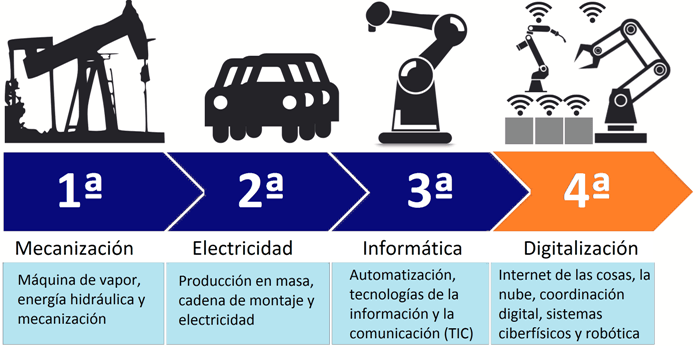
\includegraphics[width=0.6\linewidth]{./Figures/Cuarta-Revolucion-Industrial.png}
	\caption[Principales hitos de las revoluciones industriales a lo largo de la historia.]{Principales hitos de las revoluciones industriales a lo largo de la historia. \textit{Fuente: \href{https://economipedia.com}{economipedia.com}}.}
			
	\label{fig:revoluciones}
\end{figure}







Al igual que el detonante de la primera revolución industrial fue la máquina de vapor, de la segunda la producción en masa por la electricidad, y de la tercera el desarrollo de Internet, en esta cuarta revolución destaca, entre otras áreas, la Inteligencia artificial alimentada con esta enorme cantidad de datos. La Ciencia de datos es el ámbito de conocimiento que engloba las habilidades asociadas al procesamiento de datos \cite{Dhar13}. Es un ámbito multidisciplinar, representado en la \Cref{fig:cienciaDatos}, en el que participan campos como las Ciencias de la computación, la Estadística y Matemáticas y el dominio específico del problema para extraer significado de los datos. Para la construcción de modelos son necesarias varias técnicas de cada una de las disciplinas anteriores, por ejemplo: algoritmia, modelado de incertidumbre, almacenamiento, reducción de datos, optimización, etc. \cite{Bs17b}. La Ciencia de datos participa en todos los niveles y decisiones que se llevan a cabo en una organización: desde un nivel operacional, en donde únicamente se gestionan datos, hasta un nivel estratégico en donde se producen decisiones a largo plazo con relación a los datos analizados, mediante el empleo de técnicas enmarcadas dentro de la Minería de datos \cite{Shearer2000}.

\begin{figure}[!hbtp]
	\def\firstcircle{(0,0) circle (4.5cm)}
	\def\secondcircle{(60:4.5cm) circle (4.5cm)}
	\def\thirdcircle{(0:4.5cm) circle (4.5cm)}
	\centering
	\resizebox{0.5\linewidth}{!}{
	\begin{tikzpicture}
	\begin{scope}[shift={(3cm,-5cm)}, fill opacity=0.4]
	\fill[red] \firstcircle;
	\fill[green] \secondcircle;
	\fill[blue] \thirdcircle;
	\draw \firstcircle node[below,xshift=-5em,yshift = -1em,fill opacity=1.0,align=center] {\LARGE Estadística y \\[1em] \LARGE Matemáticas};
	\draw \secondcircle node [above, yshift=3em,fill opacity=1.0,align=center] {\LARGE Conocimiento Experto};
	\draw \thirdcircle node [below,xshift=5em,yshift=-1em, fill opacity=1.0,align=center] {\LARGE Ciencias de \\[1em] \LARGE la Computación};
	
	\draw \thirdcircle node[xshift=-4.8em,yshift=3em, fill opacity=1.0,align=center] {\textbf{\huge Ciencia} \\[1em] \textbf{\huge de Datos}};
	
	\draw \thirdcircle node[xshift=-5.5em,yshift=-4.5em, fill opacity=1.0,align=center] {\textbf{ \Large Machine} \\ \textbf{\Large Learning}};
	
	\draw \thirdcircle node[xshift=1em,yshift=8.5em, fill opacity=1.0,align=center] {\textbf{ \Large Software} \\ \textbf{\Large Tradicional}};
	
	\draw \secondcircle node[xshift=-6.4em,yshift=-1.7em, fill opacity=1.0,align=center] {\textbf{\Large Análisis} \\ \textbf{\Large de Datos}};
	\end{scope}
	\end{tikzpicture}
}
\caption[Disciplinas que componen la Ciencia de datos.]{Disciplinas que componen la Ciencia de datos. \textit{Fuente: elaboración propia.}}
\label{fig:cienciaDatos}
\end{figure}

El proceso de Minería de datos se puede definir como el proceso no trivial de extracción de patrones y relaciones implícitas en los datos. Este conocimiento debe ser válido, novedoso, útil y comprensible para el experto para que el proceso sea exitoso. La aplicación industrial de este proceso se conoce, en inglés, como \ac{cr} y se divide en varias fases interactivas e iterativas aplicadas en un orden concreto, representadas en la \Cref{fig:kdd}, que se detallan a continuación:



\begin{enumerate}
	\item Comprensión del negocio. En esta etapa se entienden los objetivos de negocio y los requerimientos del proyecto. Asimismo, se define el problema de minería de datos a abordar.
	
	\item Comprensión de los datos. En esta etapa se recopila el conjunto de datos inicial, en donde el experto en Ciencia de datos realiza un análisis exploratorio del problema, para poder abordarlo eficazmente.
	
	\item Preparación de datos. El objetivo de esta fase es eliminar inconsistencias o ruido, reducir o aumentar el tamaño de la muestra, así como la aplicación de cualquier método que modifique la forma de los datos para homogeneizar y maximizar la ganancia de conocimiento en las fases posteriores del proceso.
	
	\item Modelado. Este período del proceso de Ciencia de datos es el encargado de la extracción del conocimiento en sí. Se lleva a cabo mediante la creación de un modelo a partir de los datos recopilados y preprocesados anteriormente. Un modelo de conocimiento es una representación de patrones de comportamiento o relaciones entre los datos que se pueden usar, por ejemplo, para predecir, entender mejor los datos o explicar situaciones pasadas, entre otros.
	
	\item Evaluación. Se realiza la presentación del conocimiento extraído al experto de una manera comprensible. Además, se evalúa la validez del mismo. En el caso de que no se satisfagan los requerimientos de calidad o los objetivos establecidos, estos resultados servirán de retroalimentación en una nueva iteración del proceso.
	
	\item Despliegue. La fase final del proceso es la implantación de los modelos resultantes en la práctica. Además, se configura el proceso de Ciencia de datos para que se aplique de manera repetida o continua.
\end{enumerate}



\begin{figure}[!hbtp]
	\centering
	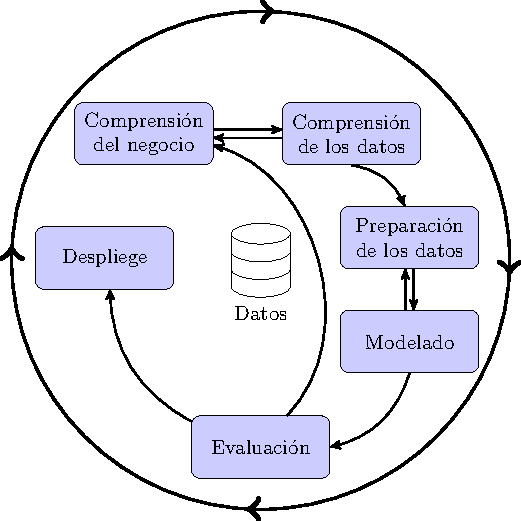
\includegraphics[width=0.5\linewidth]{./Figures/KDD2}
	\caption[Fases del proceso CRISP-DM]{Fases del proceso \ac{cr}. \textit{Fuente: elaboración propia a partir de \href{https://es.wikipedia.org/wiki/Cross\_Industry\_Standard\_Process\_for\_Data\_Mining}{https://es.wikipedia.org/wiki/Cross\_Industry\_Standard\_Process\_for\_Data\_Mining}}.}.
	\label{fig:kdd}
\end{figure}



De todas las fases del proceso de Minería de datos, el modelado es la que mayor interés ha recibido por parte de la comunidad científica, debido a que esta fase es la encargada de la extracción de valor a partir de los datos. En concreto, su cometido es la extracción de un modelo de conocimiento que represente patrones o relaciones relevantes en problemas definidos vagamente, sin una solución formal o cuyo resultado exacto conlleva un tiempo de cómputo excesivo.

Dependiendo de los objetivos establecidos en el problema a abordar, los paradigmas seguidos en Minería de datos siguen dos vertientes claramente diferenciadas: 

\begin{itemize}
	\item Predicción. Su propósito es anticipar el comportamiento de futuras entradas al sistema. Los algoritmos de Minería de datos dentro de este enfoque están basados en aprendizaje supervisado. Esto implica que los datos contienen una variable de interés que guía el proceso de extracción de patrones. Aquí se encuentran, entre otras tareas: 
	
	\begin{itemize}
		\item Clasificación \cite{Cm07}. El objetivo es predecir un valor de una variable de interés discreta. Estos valores, denominados clases o etiquetas, tienen un dominio conocido, como por ejemplo la existencia o no de una enfermedad en una serie de pacientes.
		
		\item Regresión \cite{Cm07}. Esta tarea pretende predecir el valor de una variable de interés con un dominio continuo, como por ejemplo la cantidad de precipitación en un área determinada.
		
		\item Análisis de series temporales \cite{Bjr08}. Determina el comportamiento de una variable continua a lo largo del tiempo, como por ejemplo el precio de las acciones de bolsa.
	\end{itemize}

	\item Descripción. La finalidad de este paradigma es la búsqueda de relaciones interesantes entre los datos que describan el fenómeno subyacente. Los algoritmos de Minería de datos dentro de este esquema están basados en aprendizaje no supervisado. Por lo tanto, no necesitan de una variable de interés. En este enfoque se encuentran tareas como, por ejemplo:
	
	\begin{itemize}
		\item Agrupamiento \cite{McQ67}. Consiste en la realización de grupos de instancias de datos similares entre sí y diferentes a las del resto de grupos realizados.
		
		\item Asociación \cite{Ais93}. Descubre relaciones de interés entre las diferentes variables de un conjunto de datos. 
		
		\item Detección de anomalías \cite{Hawkings98}. Identifica aquellas instancias que son inusuales o que difieren significativamente de la mayoría, pudiendo ser potenciales instancias resultado de contaminación, error o fraude.
	\end{itemize}
\end{itemize}

A pesar de la clara diferenciación entre estos enfoques en función de los objetivos establecidos, no todas las necesidades de conocimiento se satisfacen con esta clasificación. A día de hoy, existe un conjunto de técnicas que se encuentran a medio camino entre el enfoque predictivo y descriptivo englobadas dentro del marco del descubrimiento de reglas descriptivas basadas en aprendizaje supervisado (en inglés, \ac{SDRD}) \cite{Nlw09}. El objetivo de este marco de tareas es la descripción de relaciones interesantes para los expertos supeditadas a una variable objetivo o clase. Por lo tanto, la finalidad de estas técnicas no se centra en la predicción del comportamiento de una nueva instancia en relación a una variable de interés, sino en la descripción de aquellas características o factores que provocan dicho comportamiento. 

Un ejemplo ilustrativo de aplicación de un modelo \ac{SDRD} podría ser la determinación de las circunstancias en las que un paciente puede sufrir un tipo concreto de cáncer, de modo que los investigadores sanitarios puedan acotar su investigación. En este ejemplo el objetivo no es predecir la enfermedad, sino describir aquellos factores de riesgo que pueden producirla.

Actualmente, las técnicas de Minería de datos encuadradas dentro de \ac{SDRD} más destacadas son las siguientes:

\begin{itemize} \label{it:sdrd_tasks}
	
	\item Minería de conjuntos de contraste (en inglés, \ac{CSM}) \cite{Bp01}. Tiene como finalidad la búsqueda de patrones cuyas distribuciones difieran significativamente entre diferentes grupos de objetos. Es importante destacar que estos grupos son exclusivos entre sí, por lo que una instancia únicamente puede pertenecer a uno de ellos. En concreto, un patrón será determinado como de contraste si la diferencia de soporte del patrón entre los diferentes grupos es mayor a un valor umbral establecido. Debido a esta característica, su aplicación es interesante en investigaciones de ciencias sociales, pues es muy habitual este tipo de análisis, aunque actualmente se está aplicando también a otros campos como analítica de negocio \cite{Ts09} o medicina \cite{Rgza15}, entre otros \cite{Boe11}.
	
	\item Descubrimiento de subgrupos (en inglés, \ac{SD}) \cite{Klo96, Wro97}. El objetivo de esta tarea es la descripción de subconjuntos de instancias cuya distribución estadística difiere significativamente respecto al conjunto total de la población, dada una variable de interés. Como esta tarea se centra en la búsqueda de relaciones con características interesantes, no es necesario que estas sean completas, sino que suele ser suficiente con relaciones parciales, que se describen en forma de patrones individuales. En los últimos años, esta tarea ha recibido especial interés por parte de la comunidad científica debido a su éxito en diferentes ámbitos \cite{Hcgd11}. Una revisión completa de la tarea enfocada en algoritmos evolutivos se presenta en \cite{Cgdh14}. En \cite{Atz15} puede encontrarse una revisión de métodos exhaustivos. Finalmente, en \cite{Hel16} se presenta una revisión basada en una evaluación empírica de estos modelos.
	

	
	\item Minería de patrones emergentes (en inglés, \ac{EPM}) \cite{Dl99,Dl05}. La búsqueda se basa en la obtención de aquellos patrones que sean frecuentes para una clase y poco frecuentes para el resto. Los objetivos que se pueden alcanzar con este enfoque son la búsqueda de tendencias emergentes a lo largo del tiempo y la búsqueda de características discriminativas entre las diferentes clases de un problema. Debido a esta propiedad, \ac{EPM} no solo puede utilizarse con carácter descriptivo, sino que también puede usarse de manera predictiva. De hecho, a pesar del claro enfoque descriptivo de la tarea, el empleo de patrones emergentes en la literatura ha estado principalmente enfocado a tareas de clasificación \cite{Gmc14}.
\end{itemize} 

Para alcanzar estos requerimientos, además de ser precisos, es deseable que los modelos \ac{SDRD} obtengan conocimiento que se pueda representar de un modo en el que se facilite su comprensión por parte de un ser humano, de modo que: 

\begin{enumerate}
	\item Los diseñadores y desarrolladores puedan analizar el modelo generado y entender su estructura.
	
	\item Los usuarios finales sean capaces de utilizar el modelo como un sistema de ayuda a la decisión, explicando el fenómeno que subyace en los datos para así tomar mejores decisiones y permitiendo justificarlas más fácilmente.
\end{enumerate}

Una manera simple de combinar ambos aspectos es mediante la utilización de conjuntos de patrones y/o reglas, las cuales se emplean en \ac{SDRD}. No obstante, el principal hándicap es la extracción eficiente de dichos patrones. Para la mayoría de problemas actuales, la aplicación de estos métodos es inviable debido a las altas dimensiones que poseen los datos de entrada. En este contexto un procesamiento distribuido se vuelve obligatorio. Recientemente se han desarrollado diversas plataformas, herramientas y paradigmas para el procesamiento de datos masivos, facilitando al usuario final el desarrollo de métodos en entornos distribuidos. La principal ventaja de estos sistemas  es la gestión transparente al usuario de los recursos y mecanismos necesarios para el correcto funcionamiento de un procedimiento dentro de un entorno distribuido.






De hecho, actualmente el análisis de datos masivos, conocido como \textit{big data} \cite{Frlbdbh14}, se aplica en prácticamente cualquier ámbito: educación \cite{Hwhhz19}, ciudades inteligentes \cite{Xclwx16,Sbkt19}, seguridad \cite{Plyyl17}, entre otros \cite{Dlczh18,Btmpgpsp19,Mhzvl19}. Esto se debe principalmente a la proliferación de herramientas capaces de manejar estos datos masivos de manera eficaz y eficiente. Entre estos, uno de los paradigmas de computación más populares es MapReduce \cite{Dg08}. Este se basa en un marco de programación funcional basado en el paradigma ``divide y vencerás'' para el procesamiento distribuido de \textit{big data}. 



Los modelos \ac{SDRD} son especialmente interesantes en el ámbito \textit{big data} ya que permiten obtener una descripción simplificada, fiable y altamente comprensible de los fenómenos que subyacen sobre la inmensa cantidad de información que se está procesando. No obstante, los desarrollos actuales para la extracción de modelos \ac{SDRD} sufren con el crecimiento en la dimensión de los datos ya que la mayoría no están diseñados para un procesamiento distribuido. En consecuencia, su rendimiento decae significativamente o es imposible su aplicación. Por lo tanto, el desarrollo de métodos de extracción de modelos \ac{SDRD} con un diseño distribuido es actualmente un reto importante en la comunidad científica.

Pero no sólo se requiere procesar grandes conjuntos de datos estáticos. Debido al avance en los últimos años en la tecnología, protocolos y aplicaciones empleados en el denominado Internet de las Cosas (en inglés, \ac{IoT}) \cite{Agmaa15}, entre otros, también es necesario procesar conjuntos dinámicos e infinitos que llegan constantemente al sistema a lo largo del tiempo. A este tipo de conjunto de datos dinámico se le conoce como flujo de datos (en inglés, \textit{data stream}) \cite{Gama10}. Debido a su naturaleza, el procesamiento de flujos de datos impone una serie de restricciones añadidas a la minería de datos tradicional. Entre otras, destaca la necesidad de actualizar constantemente el modelo de aprendizaje conforme los datos llegan al sistema, así como importantes restricciones de memoria y tiempo de procesamiento de cada instancia. 

En el ámbito de la minería de flujo de datos, los modelos \ac{SDRD} son muy interesantes para el experto debido a sus características. Entre otras aplicaciones, estos modelos de aprendizaje pueden ser utilizados para proporcionar un resumen del estado actual del flujo de datos, describiendo aquellos aspectos más interesantes para el experto. También son útiles para la identificación de los elementos que han propiciado un cambio en los datos, o pueden utilizarse para la descripción de tendencias emergentes en los datos. Sin embargo, la mayoría de métodos \ac{SDRD} desarrollados no tienen en cuenta todas las restricciones presentes en la minería de flujo de datos. No obstante, algunos de estos procedimientos se basan en métodos incrementales para administrar flujos estáticos y finitos, como por ejemplo en \cite{Fr02,Fr06,Lshz14}. Pero la principal dificultad que se encuentra a la hora de realizar una adaptación directa de las técnicas de extracción de modelos \ac{SDRD} se basa en el empleo de medidas de calidad y esquemas de aprendizaje que asumen la invariabilidad de las propiedades de los datos a lo largo del tiempo, así como la disponibilidad de la totalidad de los datos desde el inicio. Por lo tanto, se hace indispensable el desarrollo de modelos SDRD capaces de actualizarse a lo largo del tiempo, teniendo en cuenta la naturaleza cambiante de los flujos de datos.


\subsection*{Objetivos}

Con estas premisas, se establece como hipótesis de partida que el uso de modelos \ac{SDRD} para la extracción de conocimiento en problemas complejos ayuda a cubrir satisfactoriamente las necesidades de conocimiento que demandan los expertos en este tipo de entornos. Para ello, el objetivo principal asociado será el análisis y desarrollo de diferentes modelos \ac{SDRD} para entornos \textit{big data} y flujos continuos de datos. Este objetivo principal se subdivide en los siguientes objetivos específicos:

\begin{itemize}
	\item Estudio e identificación de los principales enfoques utilizados en \ac{SDRD} para problemas complejos. 
	
	\item Desarrollo de nuevas propuestas algorítmicas para la extracción de modelos \ac{SDRD} capaces de obtener conocimiento altamente representativo del conjunto de datos analizado y fácilmente comprensibles por parte de los expertos. 
	
	\item Análisis, diseño y desarrollo de propuestas para la extracción de conocimiento en entornos \textit{big data} bajo el paradigma MapReduce.
	
	\item Análisis, diseño y desarrollo de propuestas para la extracción de conocimiento altamente descriptivo en entornos de flujos de datos.
	
	\item Aplicación de las propuestas a datos reales con el objetivo de transferir los resultados de investigación al sector productivo y a la sociedad en general.
\end{itemize}


\subsection*{Estructura de la memoria}

En virtud con lo establecido en el artículo 25, punto 2 de la normativa vigente para los Estudios de Doctorado de la Universidad de Jaén, correspondiente al programa establecido en el RD. 99/2011, esta tesis doctoral se presenta como un compendio de artículos publicados por el doctorando. Por consiguiente, y tras el capítulo introductorio, esta memoria se estructura de la siguiente manera:

\begin{itemize}


	\item En el \Cref{chap:background} se introducen los detalles de los principales conceptos que se abordan en esta tesis doctoral como \ac{SDRD}, computación flexible, en donde se hace especial hincapié en los sistemas difusos evolutivos y sus componentes, y los problemas complejos dentro de la Ciencia de datos.
	
	\item El \Cref{chap:discusion} presenta una descripción general de las ideas propuestas en los trabajos realizados por el doctorando, destacando las características principales de las mismas, junto a una discusión de los resultados obtenidos.
	
	\item El \Cref{chap:conclusion} expone las principales conclusiones extraídas, los trabajos futuros que se derivan del trabajo realizado en esta tesis, así como las publicaciones asociadas con el trabajo principal de investigación.
	
	\item Finalmente, en el \Cref{chap:publications} se presentan las publicaciones indexadas en el \ac{JCR}, fruto del trabajo realizado en esta tesis, las cuales conforman el núcleo de la investigación realizada.
\end{itemize}






%
\clearpage{} \cleardoublepage

\rhead[ ]{\sc{Introduction}}
\lhead[\sc{Introduction}]{} 	

\rhead[\footnotesize{\sc{Cap\'itulo \thechapter: \rm\leftmark}}]{}   \lhead[ ]{\footnotesize{\sc{\thesection: \rm\rightmark}}}  

\renewcommand{\figurename}{Figura}
\renewcommand{\tablename}{Tabla}

\clearpage{}

\acused{SDRD}
\acused{IoT}
\acused{EPM}
\acused{SD}
\acused{XAI}

\chapter{Conceptos teóricos} \label{chap:background}

En este capítulo se describen en detalle los conceptos principales que se utilizan a lo largo de esta memoria. En concreto, en el \Cref{sec:sdrd} se presentan los conceptos principales del marco de tareas \ac{SDRD}. Después, en el \Cref{sec:flexible} presenta el paradigma de la computación flexible, centrándose en la lógica difusa, los algoritmos evolutivos y la hibridación de ambos: los sistemas difusos evolutivos. A continuación, el \Cref{sec:complejos} presenta los detalles de problemas complejos como aprendizaje multi-instancia en el \Cref{sec:MIL_BG}, \textit{big data} en el \Cref{sec:bigdata} y las características más destacadas de los flujos de datos en el \Cref{sec:ds}.

\section{Extracción de reglas descriptivas mediante aprendizaje supervisado} \label{sec:sdrd}

Tradicionalmente, la minería de datos ha tenido dos paradigmas de aprendizaje claramente diferenciados: supervisado y no supervisado. En general, los algoritmos basados en aprendizaje supervisado tienen un enfoque más predictivo, mientras que los enfoques no supervisados tienden a un enfoque más descriptivo de los datos de entrada. Sin embargo, estos modelos no son suficientes para cubrir todas las necesidades de conocimiento que se demandan en la actualidad.

\ac{SDRD} \cite{Nlw09} es un área de investigación que aglutina a todas las técnicas de minería de datos capaces de obtener conocimiento descriptivo relacionado con una variable de interés para el usuario, mediante el uso de patrones o reglas. El objetivo es la descripción de las características que producen el valor de la variable objetivo. Por ejemplo, en el estudio de un tipo de cáncer, \ac{SDRD} no pretende predecir si un nuevo paciente puede tener la enfermedad, sino describir aquellos factores más relevantes que lo producen. 

Una definición clásica de patrón se puede encontrar en \cite{Ms82} como: sea $I = \lbrace i_1, i_2,...,i_n \rbrace$ un conjunto de selectores. Un selector se define mediante una tripleta $(v, r, S)$, donde $v$ es una variable del problema; $r$ es un operador relacional, como por ejemplo $=,\neq,\in,\notin,>,<,\geq,\leq$, entre otros; y S es un valor o conjunto de valores pertenecientes al dominio de la variable $v$. Uno de estos selectores será la variable objetivo del problema, denominada $v_c$. Esta definición de patrón, establecida anteriormente al desarrollo de \ac{SDRD}, sigue manteniéndose vigente en este ámbito. Por tanto, un patrón $P$ de un modelo \ac{SDRD} se representa como: 

\begin{equation}
P: C \rightarrow v_c
\end{equation}

\noindent donde $v_c$ es el valor de la variable objetivo y $C \subseteq I$.  Los selectores presentes en $C$ suelen representarse unidos mediante conjunciones o en forma normal disyuntiva (en inglés, \ac{DNF}) para una representación más compacta.


Como se ha comentado anteriormente, la finalidad de \ac{SDRD} se centra en la comprensión del fenómeno subyacente que determina el valor de la variable de interés. De este objetivo se puede deducir que no es necesaria la extracción de relaciones completas, sino que con relaciones parciales que sean relevantes o interesantes es suficiente. De hecho, estas relaciones deben ser analizadas y tratadas de manera individual por parte del experto, por lo que es interesante que el solapamiento entre los patrones extraídos sea el menor posible para evitar redundancias.


De entre las técnicas enmarcadas dentro de \ac{SDRD} (véase Página \pageref{it:sdrd_tasks}), esta tesis se centra en \ac{SD} y en \ac{EPM} debido a su diversidad de aplicaciones reales. Por lo tanto, a continuación se presentan:

\begin{enumerate}
	\item Las características que deben tener los modelos \ac{SDRD}, haciendo especial hincapié en las medidas de calidad utilizadas. La gran cantidad de medidas establecidas a lo largo de la literatura para determinar la calidad de los patrones desde diferentes puntos de vista hace que sea un factor fundamental a la hora de guiar el proceso de búsqueda. Por lo tanto, se hace obligatorio la determinación de aquellas que resultan más interesantes. 

	\item Se presenta una introducción del concepto de \ac{SD}, en donde se presentarán los principales objetivos, enfoques y herramientas utilizadas a lo largo de la literatura.
	
	\item Finalmente, el tercer concepto que se introduce en esta memoria es \ac{EPM}, analizando el problema y los enfoques más empleados para la extracción de conocimiento.
\end{enumerate}




\subsection{Medidas de calidad en el marco de descubrimiento de reglas descriptivas basadas en aprendizaje supervisado}

Es deseable que el conocimiento extraído en \ac{SDRD} muestre un buen balance entre generalidad, precisión, interés e interpretabilidad de los modelos, de modo que estos sirvan como herramienta de apoyo a las decisiones finales del usuario. Este enfoque supone que, además de las particularidades de cada una de las tareas que se engloban dentro del \ac{SDRD}, se deben de optimizar varios objetivos de manera simultánea. Además, dichos objetivos a optimizar son contrapuestos entre sí \cite{Bg94}, por lo que el problema de la extracción de patrones descriptivos mediante aprendizaje supervisado se torna en un problema multiobjetivo.

Todos estos objetivos deben ser definidos para determinar la calidad de los patrones obtenidos por los modelos \ac{SDRD} y para guiar los procesos de búsqueda de forma adecuada. Sin embargo, no existe un claro consenso sobre qué medida de calidad es la más adecuada para la determinación de los diferentes objetivos \cite{Cgdh14}. Por esta razón, en la literatura se han definido una gran cantidad de métricas para determinar la calidad del conocimiento extraído \cite{Lmcg16,Glmc17}. Todas estas medidas pueden ser determinadas a partir de los valores de una tabla de contingencias, en donde se muestra el número de ejemplos correcta e incorrectamente cubiertos y no cubiertos para cada uno de los patrones extraídos. Este tipo de tabla se presenta en la \cref{tab:tablaContingencia}.

\begin{table}[!hbtp]
	\centering
	\caption{Tabla de contingencia de un patrón.}
	\begin{tabular}{c|cc}
		& Clase & No Clase \\ \hline
		Cubierto & $tp$ & $fp$ \\
		No cubierto & $fn$ & $tn$ \\ \hline
	\end{tabular} 
	\label{tab:tablaContingencia}
\end{table}

En esta tabla se define $tp$ como el número de instancias correctamente cubiertas, es decir, que satisfacen tanto el antecedente como el consecuente del patrón. El valor de $fp$ es el número de instancias que cumplen el antecedente, pero no el consecuente del patrón. El valor de $fn$ es el número de instancias que no cumplen el antecedente del patrón, pero satisfacen el consecuente. Finalmente, $tn$ se refiere al número de instancias que no cumplen ni con el antecedente, ni con el consecuente del patrón.

Entre los esfuerzos llevados a cabo para establecer un consenso en las métricas a utilizar, destaca el análisis llevado a cabo en \cite{Cdh18} en donde se establece una conexión directa entre las técnicas más relevantes de \ac{SDRD} y la medida de atipicidad o \ac{WRAcc}. Dicha medida se define en la \Cref{eq:WRAcc}:

\begin{equation}\label{eq:WRAcc}
WRAcc(P) = \frac{tp+fp}{tp+fp+fn+tn} \left(\frac{tp}{tp+fp} - \frac{tp+fn}{tp+fn+fp+tn}\right)
\end{equation}

Esta métrica presenta complejidades a la hora de realizar comparativas entre patrones de diferentes clases, pues posee una dependencia directa con el porcentaje de instancias que pertenecen a la misma. Por tanto, se hace necesaria una normalización de la medida, la cual se define en la \Cref{eq:WRAccNorm}:



\begin{equation}\label{eq:WRAccNorm}
WRAcc_{Norm}(P) = \frac{WRAcc(P) - \left(1 - \%Pos \right) \left(0 - \%Pos\right)}{\%Pos \left(1 - \%Pos\right) - \left(1 - \%Pos\right)\left(0 - \%Pos\right)}
\end{equation}

\noindent donde $\%Pos = \frac{tp + fn}{tp+fp+tn+fn}$ es el porcentaje de instancias pertenecientes a la clase objetivo del problema. Tras esto, la métrica pasa de un dominio variable que contiene valores negativos al dominio [0,1], permitiendo establecer comparativas en estudios, de manera que:

\begin{itemize}
	\item $P$ es irrelevante si $WRAcc_{Norm}(P) \leq 0.5$.
	\item $P$ es de interés si $WRAcc_{Norm}(P) > 0.5$ y además, cuanto mayor sea este valor, mayor será su ganancia de precisión.
\end{itemize}

Un análisis en profundidad y pormenorizado de las características de la medida WRAcc en las tareas de \ac{SDRD} se encuentra en \cite{Cdh18}.

Asimismo, existen diferentes estudios en el contexto de \ac{SDRD} donde se analizan una gran cantidad medidas de calidad \cite{Glmc13,Glmc17}. Atendiendo a los resultados presentados en estos estudios, las métricas que pueden utilizarse para definir los diferentes objetivos son las siguientes: 

\begin{itemize}
	\item Precisión. Es el objetivo más importante pues los patrones deben definir de manera fiable las relaciones descritas. Por ello, se establecen varias métricas:
	
	\begin{itemize}
		\item Confianza. Determina la precisión del patrón con respecto a las instancias que ha cubierto. Se calcula como se describe en la \Cref{eq:conf} \cite{Fay96}.
		
		\begin{equation} \label{eq:conf}
		Conf(P) = \frac{tp}{tp + fp}
		\end{equation}
		
		\item Índice de crecimiento (en inglés, \ac{GR}). Determina la capacidad discriminatoria del patrón al calcular el ratio de soporte entre las diferentes clases. Se calcula como se describe en la \Cref{eq:gr2}.
		
		\begin{equation}
		GR(P) = 
		\begin{cases}
		0, & \text{Si}\ fp\left(tp+fn\right) = tp\left(fp+tn\right) = 0, \\
		\infty, & \text{Si}\ fp\left(tp+fn\right) = 0 \wedge tp\left(fp+tn\right) \neq 0, \\
		\frac{tp\left(fp+tn\right)}{fp\left(tp+fn\right)}, & \text{en otro caso}
		\end{cases}
		\label{eq:gr2}
		\end{equation}
		
		\item Tasa de falsos positivos (en inglés, \ac{FPR}). Calcula el porcentaje de instancias incorrectamente cubiertas con respecto al total que no pertenecen a la clase objetivo. De este modo, nos permite determinar la magnitud de los errores de precisión del patrón. Es importante destacar que esta métrica debe ser minimizada. Se calcula como se presenta en la \Cref{eq:fpr} \cite{Gl02a}.
		
		\begin{equation} \label{eq:fpr}
		FPR(P) = \frac{fp}{fp + tn}
		\end{equation}
		
	
	\end{itemize}
	
	\item Interés. Pretende extraer conocimiento que sea novedoso, sorprendente o útil para el experto. Para ello, las métricas más utilizadas para determinar el interés de un patrón son:
	
	\begin{itemize}
		
		\item   \ac{WRAcc}, presentado en la \Cref{eq:WRAcc}. Esta medida busca un balance entre el número de instancias cubiertas por un patrón y la ganancia de precisión respecto al porcentaje de la clase. Por lo tanto, cuanto más alto sea este valor, más interesante será el patrón, pues se obtiene una mayor precisión influyendo sobre más instancias del problema.
		
		\item Índice de Jaccard (Jacc). Esta medida se utiliza para determinar la similitud entre dos conjuntos de elementos. En concreto, estos son el formado por las instancias que pertenecen a la clase y por las instancias cubiertas por el patrón, respectivamente. Esta medida ayuda a encontrar patrones interesantes con un buen balance entre generalidad y fiabilidad. Se calcula como se presenta en la \Cref{eq:jacc} \cite{Tks02}.
		
		\begin{equation} 
		\label{eq:jacc}
		Jacc(R) = \frac{tp}{tp+fp+fn}
		\end{equation}
		
		
		
	\end{itemize}
	
	
	\item Generalidad. Se busca que la cobertura de un patrón respecto a la totalidad de instancias de un problema sea máxima. Por lo general, una de las métricas más empleadas para determinar este objetivo es la tasa de verdaderos positivos (en inglés, \ac{TPR}). Esta medida cuantifica el porcentaje de instancias correctamente cubiertas por el patrón con respecto a la totalidad de ejemplos pertenecientes a la clase del patrón. Esta medida se define según se presenta en la \Cref{eq:tpr} \cite{Klo96}.
	
	\begin{equation} \label{eq:tpr}
	TPR(P) = \frac{tp}{tp + fn}
	\end{equation}
	
	
	\item Interpretabilidad. En este objetivo se pretende minimizar la complejidad del modelo de patrones extraído. Se pretende así que sea más fácil y rápido analizar y entender el conocimiento extraído para mejorar la toma de decisiones. En un modelo \ac{SDRD}, las métricas de complejidad más utilizadas son el número de patrones extraídos y el número medio de selectores o variables que forman parte del antecedente de un patrón.
	
\end{itemize}


Se puede observar que el empleo de una u otra medida de calidad va a depender del contexto de aplicación particular. No obstante, en líneas generales, es interesante remarcar la capacidad de la medida \ac{WRAcc} no solo para encontrar patrones interesantes de una manera robusta, sino para relacionar las diferentes técnicas de \ac{SDRD} entre sí \cite{Cdh18}. Asimismo, se destaca el índice de Jaccard por su gran capacidad de obtener patrones interesantes, especialmente en problemas con desbalanceo de clases \cite{Lmcg16}, muy comunes en \textit{big data} o flujos continuos de datos. Por lo tanto, dichas métricas pueden ser empleadas como base para guiar procesos de búsqueda de patrones. También se remarca el empleo de otras medidas específicas para cada uno de los objetivos de \ac{SDRD}. El empleo de estas métricas en la etapa de búsqueda puede ayudar a crear sinergias con las descritas anteriormente. Por otro lado, su empleo en la evaluación de resultados puede permitir obtener conclusiones desde diferentes puntos de vista. Por ejemplo, empleando \ac{TPR} se puede determinar el alcance global de la cobertura de un patrón. Unido a lo anterior, puede ser interesante el empleo a su vez de medidas como la confianza y el \ac{FPR}, o similares, que permitan determinar la precisión del patrón a nivel local, es decir, respecto al número de ejemplos cubiertos, y a nivel global, es decir, respecto al total de datos.

\subsection{Descubrimiento de subgrupos}

\ac{SD} \cite{Klo96,Wro97} se define como la búsqueda de subconjuntos de la población cuya distribución estadística con respecto a una variable objetivo difiera significativamente respecto al conjunto total de la población. Esta desviación hace que los subgrupos generados sean interesantes para el experto. En particular, la tarea lo que pretende es la búsqueda de aquellos subgrupos más interesantes. Estos, entre otras características, son los que influyen en el mayor número de instancias posible con la distribución estadística más inusual. 


En los últimos años, \ac{SD} ha sido ampliamente analizado por la comunidad científica \cite{Hcgd11,Cgdh14,Atz15} en donde han surgido propuestas basadas en algoritmos clásicos como AprioriSD \cite{Kl06}, SD-Map \cite{Ap06} o MergeSD \cite{Grw08}; basadas en programación genética como CGBA-SD \cite{Lrrv14}; y basadas en sistemas difusos evolutivos como SDIGA \cite{Dghm07}, MESDIF \cite{Dgh07}, NMEEF-SD \cite{Cgdh10}, FuGePSD \cite{Crdwgge15}. También hay que destacar enfoques para el análisis \textit{big data} basados en algoritmos exactos como AprioriK-SD-OE o PFP-SD-OE \cite{Plv17b}, y basados en sistemas difusos evolutivos como MEFASD-BD \cite{Prpgcd16}. Es importante destacar que, hasta donde se conoce, no se han realizado implementaciones para \ac{SD} enfocadas a la extracción de conocimiento en flujos de datos.

Uno de los aspectos más relevantes a la hora de solucionar un problema mediante \ac{SD}, es la influencia de factores externos, como ruido o presencia de datos perdidos, que pueden afectar negativamente en la calidad del conocimiento extraído. En este sentido, en la literatura se ha analizado el comportamiento de los algoritmos con respecto a valores perdidos \cite{Clgd12}. Asimismo, factores internos como la redundancia en los patrones extraídos provoca un decremento de la calidad del conocimiento extraído. En este aspecto, los investigadores de la literatura sí han analizado el problema y se han propuesto diversas soluciones al mismo \cite{Lltsss14,Lpdk15}.

Finalmente, es importante destacar que actualmente se encuentran disponibles para la comunidad científica muchos paquetes desarrollados para distintas plataformas de software abierto. Por ejemplo, existe un paquete con algoritmos clásicos de \ac{SD} desarrollado para la herramienta R denominado \textit{rsubgroup}\footnote{\url{https://cran.r-project.org/web/packages/rsubgroup/index.html}}. También están disponibles paquetes de algoritmos integrados en las herramientas KEEL\footnote{\url{http://keel.es}} \cite{KEEL3} y Orange\footnote{\url{http://kt.ijs.si/petra\_kralj/SubgroupDiscovery}} \cite{Orange}.

\subsection{Minería de patrones emergentes}

\ac{EPM} \cite{Dl99,Gcmgj18} tiene como objetivo la búsqueda de patrones que describen un alto número de instancias de una clase determinada, minimizando la inclusión de elementos que no pertenecen a dicha clase. Por lo tanto, el patrón tendrá un soporte muy alto para una clase y muy bajo para el resto. Así, la tarea intenta buscar patrones con un gran poder discriminatorio.

En concreto, la minería de patrones emergentes se define como la búsqueda de aquellos patrones $P$ cuyo \ac{GR} entre dos conjuntos de datos, o dos clases, sea mayor a un valor umbral preestablecido $\rho > 1$. Este \ac{GR} se calcula siguiendo la fórmula presentada en \Cref{eq:gr} \cite{Dl99}.

	\begin{equation}
GR(P) = 
\begin{cases}
0, & \text{Si}\ fp\left(tp+fn\right) = tp\left(fp+tn\right) = 0, \\
\infty, & \text{Si}\ fp\left(tp+fn\right) = 0 \wedge tp\left(fp+tn\right) \neq 0, \\
\frac{tp\left(fp+tn\right)}{fp\left(tp+fn\right)}, & \text{en otro caso}
\end{cases}
\label{eq:gr}
\end{equation}

\noindent donde $tp$, $fp$, $tn$ y $fn$ son los valores de la tabla de contingencias presentada en la \cref{tab:tablaContingencia}. 


Con estas características, los principales objetivos abordados por \ac{EPM} son la búsqueda de patrones que describen características discriminatorias entre clases de un conjunto de datos, la búsqueda de tendencias emergentes a lo largo del tiempo o la diferenciación a través de un grupo de variables. 

A lo largo de la literatura se han ido desarrollando una amplia variedad de paradigmas y algoritmos de extracción de patrones emergentes, entre los que destacan el algoritmo DeEPs \cite{Ldrw04} como un método de extracción basado en límites; el algoritmo StrongJEP \cite{Fr06} o Tree-based JEP \cite{Bmr02}, como enfoques basados en árboles, entre otros. No obstante, a pesar de las capacidades descriptivas de estos patrones, los investigadores han centrado sus esfuerzos en el aspecto predictivo de los mismos \cite{Gmc14}. Es decir, de los factores que son deseables en un modelo \ac{SDRD} (generalidad, precisión, interés e interpretabilidad), únicamente se ha analizado en profundidad la precisión, ignorando prácticamente el resto de cualidades. También ha habido grandes esfuerzos en el área para paliar la influencia del ruido en los datos \cite{Bmr03,Fr04,Fr06,Rf07}. 

Recientemente, la comunidad científica ha estado más interesada en otros aspectos de la tarea y se han presentado propuestas como el algoritmo FEPM \cite{Gmc11}, el cual hace uso de lógica difusa para mejorar la interpretabilidad; o el algoritmo EvAEP \cite{Gmacd16}, basado en un sistema difuso evolutivo que intenta obtener un balance entre todos los aspectos de los modelos \ac{SDRD}. Sin embargo, hasta donde se sabe, no se ha presentado ninguna propuesta para extraer patrones emergentes en problemas complejos como \emph{big data} o flujos continuos de datos.



\section{Inteligencia computacional} \label{sec:flexible}

La Inteligencia computacional \cite{Konar05} es un amplio abanico de áreas que se incluyen dentro del campo de la Inteligencia artificial centradas en el diseño de sistemas inteligentes capaces de resolver problemas complejos. Estos se encuentran habitualmente inspirados en fenómenos de la naturaleza o en el razonamiento lingüístico humano, ya que poseen una alta tolerancia hacia la imprecisión e incertidumbre, lo que les confiere una gran capacidad de adaptación a entornos cambiantes de manera robusta. Entre otras, las áreas más destacadas que se incluyen dentro de la Inteligencia computacional son los sistemas difusos \cite{Zad65,Zad75}, los modelos probabilísticos \cite{As00}, los algoritmos de optimización bioinspirados como la computación evolutiva \cite{Bfm97} y las redes neuronales artificiales \cite{Gol96}.

Esta tesis doctoral se centra en el desarrollo de sistemas basados en reglas difusas, los algoritmos evolutivos y la combinación de ambas técnicas en los sistemas difusos evolutivos orientados a \ac{SDRD}, debido al éxito que han tenido estas técnicas en tareas como \ac{SD} y a su alta interpretabilidad. Dichas técnicas se describen con detalle en las siguientes secciones.

\subsection{Sistemas basados en reglas difusas}

La lógica difusa tiene como finalidad modelar el conocimiento impreciso y cuantitativo, así como la posibilidad de manejar la incertidumbre, con el fin de adaptar este conocimiento de una forma más cercana al razonamiento humano. Fue introducida por Zadeh \cite{Zad65,Zad75} y se fundamenta en el concepto de conjunto difuso. Un conjunto difuso es una generalización de los conjuntos clásicos, en los que un elemento $x$ cualquiera únicamente puede estar o no estar en un conjunto $S$. Por lo tanto, la función de pertenencia $\mu(x)$ se define como:

\begin{equation}
\mu(x) = 
\begin{cases}
0, & \text{Si}\ x \notin S, \\
1, & \text{Si}\ x \in S
\end{cases}
\label{eq:pertenecia}
\end{equation}

Como se puede observar, la función de pertenencia en conjuntos clásicos únicamente posee dos valores. En contraposición, una función de pertenencia sobre un conjunto difuso puede adquirir cualquier valor dentro del intervalo $[0,1]$. Esto permite que un elemento $x$ pueda pertenecer a varios conjuntos difusos en mayor o menor medida. Asimismo, se permiten representar límites difusos, pero con un significado mucho más preciso en aplicaciones reales. En \cite{Ky95} se puede encontrar una descripción detallada sobre la teoría de conjuntos difusos.

No obstante, uno de los mayores potenciales de los conjuntos difusos es la creación de variables lingüísticas a partir de variables de tipo numérico. Para ello se establece un conjunto de valores lingüísticos y se define el significado de cada uno de ellos a partir de un conjunto difuso, utilizando solapamiento entre ellos \cite{Zad75}. De este modo, una variable numérica se puede tratar mediante términos lingüísticos, como \textit{Bajo, Medio} y \textit{Alto}, los cuales tienen cierto solapamiento entre sí. Cada uno de estos términos es especificado mediante un conjunto difuso, el cual tendrá una función de pertenencia asociada. De este modo, se puede saber de manera precisa el grado de pertenencia de cualquier valor de la variable a cada uno de los términos lingüísticos especificados. En la \Cref{fig:conjuntoDifuso} se muestra un ejemplo de una partición difusa para una variable numérica considerando cinco etiquetas lingüísticas: \textit{Muy bajo, Bajo, Medio, Alto} y  \textit{Muy alto}, donde \textit{Bajo, Medio} y \textit{Alto} tienen una función de pertenencia triangular y el resto una función de pertenencia trapezoidal.


\begin{figure}[!hbtp]
	\centering
	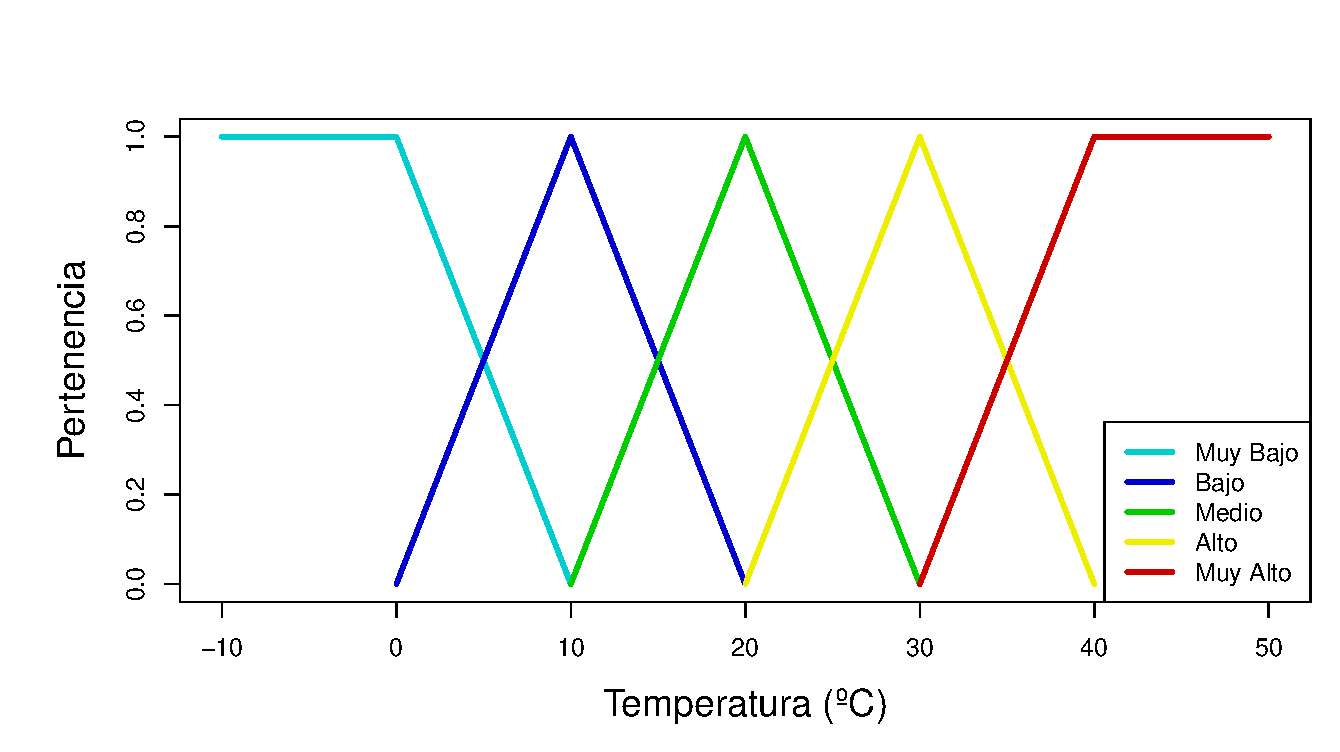
\includegraphics[width=0.8\linewidth]{./Figures/fuzzy.pdf}
	\caption[Ejemplo de definición de la variable \textit{Temperatura} con cinco etiquetas lingüísticas.]{Ejemplo de definición de la variable \textit{Temperatura} con cinco etiquetas lingüísticas. \textit{Fuente: elaboración propia.}}
	\label{fig:conjuntoDifuso}
\end{figure}

Esta expresividad que poseen los conjuntos difusos permite la simplificación de reglas y sistemas que utilizan lógica difusa. Los sistemas basados en reglas que emplean lógica difusa se denominan sistemas basados en reglas difusas \cite{Hul05,Hul11}. Estos son una extensión de los sistemas de reglas clásicos, en donde se emplean una base de reglas ``SI-ENTONCES'' donde tanto en la parte del antecedente, como en el consecuente, se considera el empleo de lógica difusa. Por esta razón, además del conjunto de reglas, estos sistemas deben almacenar información relativa a la definición de los diferentes términos lingüísticos establecidos para cada variable. Los sistemas basados en reglas difusas han demostrado su habilidad para enfrentarse a diferentes problemas como control, clasificación, minería de datos, etc. Los trabajos pioneros de aplicación de estos sistemas a estos problemas se pueden observar en \cite{Wm92,Ped96,Palm97,Kun2000,Inn04}.

Dentro de los sistemas basados en reglas se pueden emplear diferentes esquemas para su representación. Las más habituales son la representación canónica y la representación \ac{DNF}. En la primera, el antecedente de una regla es creado mediante pares variable-valor unidos por conjunciones. Por lo que una variable podrá tener únicamente un valor. Por el contrario, la representación \ac{DNF} permite una mayor flexibilidad permitiendo que una variable pueda tener varios valores al mismo tiempo, unidos mediante disyunciones, mientras que la unión entre las diferentes variables del antecedente se realiza mediante conjunciones. Un ejemplo de reglas canónicas y \ac{DNF} se muestra en las \Cref{eq:can,eq:dnf}, respectivamente.

\begin{equation}
\label{eq:can}
P_{can}:SI~v_1 = \mathit{Bajo} \wedge v_3 = \mathit{Medio}~~ENTONCES~~ v_c
\end{equation}

\begin{equation}
\label{eq:dnf}
	P_{dnf}:SI~v_1 = \left(\mathit{Bajo} \vee \mathit{Medio} \right) \wedge v_3 = \mathit{Medio}~~ENTONCES~~v_c
\end{equation}


Para aplicar una regla difusa en una instancia concreta, es necesario que el grado de compatibilidad con el antecedente de la regla sea mayor a un umbral $\alpha$ preestablecido. Esto implica que la instancia se encuentra dentro de la zona del espacio que describe la regla. Dicho grado de compatibilidad se calcula según se indica en la \Cref{eq:apc}.

\begin{equation} \label{eq:apc}
APC(e, P) = T\left( TC\left(\mu_1^1(e_1),...,\mu_n^1(e_k)\right) , ... , TC\left(\mu_1^k(e_1),...,\mu_n^k(e_k)\right)  \right)
\end{equation}

\noindent donde: 

\begin{itemize}
	\item $e_k$ indica el valor de la variable $v_k$ en la instancia $e$.
	\item $\mu_n^k$ indica la función de pertenencia del término lingüístico $n$ en la variable $v_k$.
	\item $TC$ indica la aplicación de una t-conorma difusa, es decir, una operación \textit{O} difusa. Habitualmente se emplea la t-conorma máximo.
	\item $T$ indica la aplicación de una t-norma difusa, es decir, la aplicación de la operación \textit{Y} difusa. Habitualmente se emplea una t-norma mínimo.
\end{itemize}




\subsection{Algoritmos evolutivos}

La computación evolutiva \cite{Hol75,Gol89} se basa en la utilización de algoritmos estocásticos inspirados en la evolución natural de las especies, o en otros procesos naturales, para problemas de optimización y búsqueda. En esta tarea se engloban numerosos paradigmas como los algoritmos genéticos \cite{Gol89}, la programación genética \cite{Koza92,Koza94} o las estrategias evolutivas \cite{Schwefel95}, entre otras.


El esquema general de funcionamiento de este tipo de algoritmos, representado en la \Cref{fig:evolutivo}, se podría resumir de la siguiente manera \cite{Mic92}: 

\begin{enumerate}
	\item Se parte de una población inicial de individuos o cromosomas, los cuales codifican un conjunto de soluciones completas o parciales al problema dado.
	
	\item Estos cromosomas irán evolucionando a lo largo del tiempo a través de la aplicación de los operadores genéticos de selección, cruce y mutación para generar una nueva población de descendientes. Mediante este proceso, se produce en la población una competición y variación controlada entre los individuos.
	
	\item Una vez creada la población de descendientes, esta sustituirá a la población de padres mediante un operador de remplazo.
	
	\item Tras esto, el proceso evolutivo volverá a empezar de nuevo. Este ciclo continua hasta que se satisfaga cierta condición de parada, como por ejemplo el número de ciclos evolutivos llevados a cabo, devolviendo la mejor o mejores soluciones encontradas al experto.
\end{enumerate}



\begin{figure}[!hbtp]
	\centering
	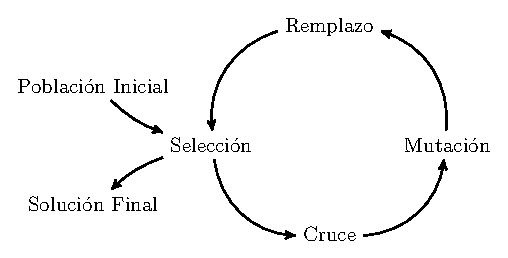
\includegraphics[width=0.8\linewidth]{./Figures/genetico_esquema.pdf}
	\caption[Esquema general de funcionamiento de un algoritmo evolutivo.]{Esquema general de funcionamiento de un algoritmo evolutivo. \textit{Fuente: elaboración propia.}}	
	\label{fig:evolutivo}
\end{figure}


Para poder resolver un problema utilizando computación evolutiva, es necesario definir una serie de elementos, los cuales se describen a continuación:

\begin{itemize}
	\item Representación de la solución en los individuos. Es el factor más importante pues va a influir en cómo el resto de mecanismos van a ser aplicados. Existen diferentes tipos de representación, entre los que destacan la codificación binaria, real o basada en orden, entre otras.
	
	\item Mecanismo de selección. Se encarga de seleccionar aquellos individuos candidatos a reproducirse para crear la población de descendientes. El uso de un operador u otro determinará la presión en la competición entre individuos, así como la convergencia del método \cite{Gd91}.
	
	\item Operadores genéticos. Son los encargados de generar la población de descendientes modificando y compartiendo la información almacenada entre los individuos de la población seleccionados previamente. Estos operadores son clave en el proceso de búsqueda pues permiten obtener un balance adecuado entre la capacidad de exploración y explotación del espacio de búsqueda \cite{Vlm13}. 
	
	\item Modelo de población o remplazo. Define cómo evoluciona la población de soluciones candidatas a lo largo del tiempo. Entre otros, los modelos  más destacados son el modelo generacional y el estacionario \cite{Es03}. 
\end{itemize}


\subsection{Sistemas difusos evolutivos}

Los sistemas basados en reglas difusas han demostrado ser una herramienta útil en un amplio número de problemas para representar el conocimiento de una manera más cercana al razonamiento humano, junto a una mejora de la robustez frente a la incertidumbre \cite{Guillaume01,Gah11, Fhcdm19}. Sin embargo, los componentes de estos sistemas se pueden mejorar mediante un proceso evolutivo de aprendizaje u optimización de modo que su comportamiento se adapte a un contexto en particular \cite{Fldh15}. La combinación entre lógica difusa y algoritmos evolutivos para la inducción de conocimiento se conoce en la literatura como sistemas difusos evolutivos y han sido exitosos en múltiples áreas de aplicación \cite{Chhm01,Cghhm04,Her08,Cor11,Fldh15,Fcdh16}.

Los sistemas difusos evolutivos se pueden dividir en dos tipos según el componente del sistema basado en reglas difusas que el algoritmo evolutivo está optimizando \cite{Her08}: algoritmos que ajustan la base de datos de términos lingüísticos, o el sistema de inferencia; y algoritmos que aprenden la base de conocimiento, la base de términos lingüísticos o todos los componentes.
 
Como se ha comentado anteriormente, el principal elemento de los algoritmos evolutivos es la representación empleada para los cromosomas. En este aspecto, las codificaciones más habituales empleadas en los sistemas difusos evolutivos para aprendizaje de reglas son:

\begin{itemize}
	
	\item El enfoque ``Cromosoma = Conjunto de reglas'', también conocido como enfoque \textit{Pittsburgh}, en donde un individuo representa un conjunto de reglas y se devuelve el mejor de ellos \cite{Smith80}.
	
	\item El enfoque ``Cromosoma = Regla'', en donde un individuo representa una única regla y el resultado final se presenta como un conjunto de diferentes individuos seleccionados según cierto criterio. Dentro de este enfoque, podemos encontrar tres propuestas diferentes para presentar este conjunto de reglas:
	
	\begin{itemize}
		
		\item El enfoque Michigan \cite{Hr78}. Un individuo representa una única regla y se devuelve toda la población. Estos sistemas se emplean habitualmente en clasificación.
		
		\item El enfoque \ac{IRL} \cite{Vent93}. En este enfoque se devuelve únicamente el mejor individuo encontrado a lo largo del proceso evolutivo. Este se ejecuta de manera iterativa hasta cumplir cierta condición de parada, formando así el conjunto de reglas final.
		
		\item El enfoque ``cooperativo-competitivo'' \cite{Gs93}. Se extrae un subconjunto de la población, de modo que los individuos por un lado compiten entre sí para no ser eliminados, pero por otro cooperan para mejorar la calidad del subconjunto de reglas final.
		
	\end{itemize}
\end{itemize}

\section{Problemas complejos en Ciencia de datos} \label{sec:complejos}

Debido a la gran cantidad de información generada a día de hoy, existe un interés elevado por parte de la comunidad hacia el diseño y desarrollo de métodos capaces de abordar esta cantidad de información en un tiempo razonable. No obstante, esto es todo un reto ya que los axiomas en los que funcionan los enfoques tradicionales ya no se sustentan en estos ámbitos. Por lo tanto, muchos problemas son inabordables desde una perspectiva tradicional.

En esta tesis se abordarán estos problemas desde el punto de vista descriptivo y por ello se profundiza en sus características en las siguientes secciones.

\subsection{Aprendizaje multi-instancia} \label{sec:MIL_BG}



En la minería de datos tradicional, cada objeto o instancia se describe inequívocamente por medio de un vector de características que se asocia, a su vez, con un valor de salida o variable objetivo. En el aprendizaje multi-instancia (en inglés, \ac{MIL}) \cite{HerreraVBCZSV16}, las estructuras de datos son más complejas. En este caso, cada valor de salida se asocia de manera ambigua con un conjunto indeterminado de vectores de características que están relacionadas con dicho valor objetivo. Un ejemplo ilustrativo se muestra en la \Cref{fig:MIL_ejemplo}. En \ac{MIL}, cada una de las instancias que comparten el valor de salida se les denomina bolsa. Es importante destacar que, cada una de las instancias individuales que conforman la bolsa tiene un valor asociado de la variable. Sin embargo, ese valor es desconocido y únicamente se conoce el valor de salida asociado con la bolsa. De hecho, a veces no todas las instancias incluidas en un bolsa son relevantes, puede haber algunas que no tengan ninguna información relevante sobre el valor de salida o que están más relacionadas con otras clases, incluyendo ruido en la información. 

\begin{figure}[!hbtp]
		\centering
	\subfloat[Aprendizaje con una única instancia.]{
		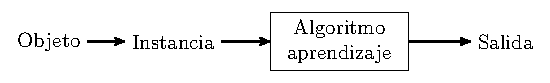
\includegraphics[width=0.75\linewidth]{./Figures/MIL1.pdf}
		\label{fig:MIL1}
	} \\
	\subfloat[Aprendizaje multi-instancia.]{
		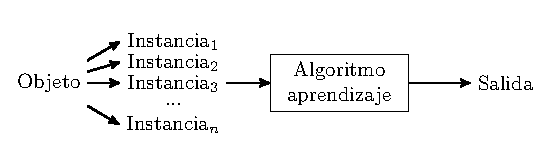
\includegraphics[width=0.75\linewidth]{./Figures/MIL2.pdf}
		\label{fig:MIL2}
	}
	\caption[Diferencia entre aprendizaje clásico y multi-instancia]{Diferencia entre un aprendizaje clásico con una única instancia y un problema \ac{MIL} \textit{Fuente: elaboración propia a partir de \cite{Lcgjv19}.}}
	\label{fig:MIL_ejemplo}
\end{figure}

Un ejemplo donde un problema \ac{MIL} se puede representar de manera natural puede ser la clasificación de imágenes. En este caso, se extraen de cada imagen diferentes zonas o regiones del espacio, pero únicamente se etiqueta la imagen de manera global. Para clasificar imágenes en donde haya una playa, se pueden extraer diferentes regiones de una imagen que representen, por ejemplo, el agua, la arena u otros elementos que pueden no corresponderse con una playa. Sin embargo, en su conjunto todas estas características extraídas en la imagen si representaría una playa.

A lo largo de la literatura se han realizado varias implementaciones de algoritmos para resolver problemas \ac{MIL}. En \cite{Amores13} se presenta una revisión de los paradigmas más destacados que se han utilizado en \ac{MIL} para extraer conocimiento de este tipo de información: 

\begin{itemize}
	\item Espacio de instancia. La información discriminadora se encuentra en el ámbito de la instancia. Esto implica que únicamente se tienen en cuenta las características que presentan las instancias. Por lo tanto, la clasificación se realiza en función de una puntuación entre instancias. A este proceso se le denomina asunción colectiva \cite{Weidmann2003}, o basada en umbral. Esta se basa en la clasificación de una bolsa como positiva (en problemas binarios) si y solo si el número de instancias clasificadas como positivas es mayor a dicho umbral. En caso contrario, la bolsa se clasificará como negativa. Si este valor umbral es igual a uno, se le denomina asunción estándar del problema \ac{MIL}.
	
	\item Espacio de bolsa. En este caso la información discriminadora recae en las características propias de la bolsa, por lo que estas son tratadas como una entidad completa. En este enfoque, el proceso de aprendizaje discrimina entre bolsas. Habitualmente se definen funciones de distancia entre bolsas para ser utilizas en clasificadores como K-NN o SVM.
	
	\item Espacio embebido. También basado en información relativa a la bolsa, este enfoque mapea información global de la bolsa a un único vector de características que la resume. Por lo tanto, cualquier algoritmo de clasificación clásico pude ser empleado.
\end{itemize}

A pesar de que el desarrollo de algoritmos para \ac{MIL} tiene un claro componente predictivo, también posee especial interés en un análisis descriptivo de los datos. Por ejemplo, dentro de un problema clásico de análisis de cesta de la compra, múltiples compras realizadas por un mismo cliente pueden estar agrupadas en la misma bolsa. En este tipo de análisis descriptivo, el enfoque \ac{MIL} no puede llevarse a cabo mediante los enfoques del espacio de bolsa y espacio embebido ya que cada instancias es relevante de manera aislada y se debería de analizar una a una para cada bolsa. Sin embargo, hasta donde alcanza nuestro conocimiento, no se ha realizado ningún desarrollo de algoritmos \ac{SDRD} para este tipo de problema.

\subsection{Big data} \label{sec:bigdata}

Según un informe de la empresa Cisco\footnote{\url{https://www.cisco.com/c/en/us/solutions/collateral/service-provider/global-cloud-index-gci/white-paper-c11-738085.html}}, para el año 2021 se espera una generación de 847 \textit{zettabytes}\footnote{1 \textit{zettabyte = $10^{21}$ bytes}} de datos. De hecho, se espera que la cantidad de datos generados sea dos órdenes de magnitud mayor que la cantidad de datos almacenados en ese mismo año. Por lo tanto, una gran cantidad de información tiene un carácter efímero. La extracción de conocimiento en estos datos masivos se ha convertido en uno de los problemas más importantes debido a que los algoritmos de minería de datos actuales son incapaces de abordar la magnitud de estos datos. Por esta razón, se necesitan tecnologías que sean capaces de recoger, mantener, transmitir y procesar grandes volúmenes de datos en un tiempo razonable. 

A esta ingente cantidad de datos se le conoce actualmente como \textit{big data}. Laney \cite{Lan01} definía el concepto como un conjunto de datos de gran volumen, que llega a gran velocidad a los sistemas de cómputo desde una gran variedad de fuentes. A esta definición, conocida como el modelo de las tres uves del \textit{big data}, se le han ido añadiendo elementos posteriormente como veracidad y valor de los datos, entre otros. En general, cualquier problema de análisis de datos que sea lo suficientemente grande y complejo como para poder ser procesado por una única máquina en un tiempo razonable puede ser definido como un problema \textit{big data}.

Para intentar mitigar los efectos de los problemas \textit{big data}, han surgido múltiples herramientas y algoritmos que hacen uso de la computación distribuida para abordar esta ingente cantidad de datos. Como resultado de la evolución de estas tecnologías, ha surgido todo un ecosistema de plataformas y técnicas para afrontar los diferentes escenarios que se pueden dar en la industria y en la ciencia \cite{Frlbdbh14}. El objetivo último de todas estas tecnologías es acercar la computación distribuida en grandes centros de computación al usuario estándar, haciendo totalmente transparente los aspectos técnicos de estos entornos.

Uno de los paradigmas de computación distribuida que más éxito ha cosechado en el análisis \textit{big data} es el paradigma MapReduce \cite{Dg04,Dg08}, así como su contraparte de código abierto, Hadoop \cite{Whi12}. La principal ventaja de este sistema es que el empleo de computación distribuida es totalmente transparente al usuario. De hecho, provee de manera automática mecanismos de tolerancia a fallos, creación de particiones de datos, así como asignación de recursos computacionales a diferentes trabajos, entre otros. 

MapReduce se basa en el paradigma divide y vencerás, llevado al ámbito de la computación distribuida. Para el diseño efectivo de un algoritmo bajo este paradigma, el desarrollador deberá dividir el procesamiento de datos en dos etapas principales: \textit{map}, y \textit{reduce}. En la primera, los datos será divididos y procesados de manera distribuida, mientras que en la segunda etapa se agregarán los resultados obtenidos en la fase anterior.

Concretamente, uno de los pilares fundamentales del paradigma es el empleo de pares clave-valor, utilizados internamente durante todo el flujo de trabajo. El funcionamiento básico del paradigma MapReduce, representado gráficamente en la \Cref{fig:mapreduce}, se define a continuación:

\begin{enumerate}
	\item En la fase \textit{map}, los datos se dividen en diferentes particiones, las cuales se envían a los diferentes nodos de cómputo, optimizando la localidad de los datos. Cada una de estas particiones se identifica con una tupla $\left(k_i, v_i\right)$ siendo $k_i$ la clave y $v_i$ los datos de la partición. A continuación, los nodos procesan de manera distribuida los datos de acuerdo a la función \textit{map} programada por el usuario. Al finalizar, se generará una nueva tupla $\left(k_i, v_i'\right)$ que contendrá resultados parciales.
	
	\item Tras esto, existe una fase intermedia, denominada \textit{shuffle}, en donde se agrupan y se ordenan los resultado parciales obtenidos anteriormente por clave, si fuera necesario. Este proceso es totalmente transparente al usuario pero debe ser tenido en cuenta en el proceso de diseño debido a su alto impacto en el rendimiento.
	
	\item Finalmente, en la fase \textit{reduce} se agregan los resultados parciales producidos por el procedimiento \textit{map}, utilizando la función \textit{reduce} programada por el usuario. Este procedimiento se ejecuta para cada clave $k_i$. El resultado final de la función es una nueva tupla $\left(k_i,v_i''\right)$ que contendrá el resultado final para cada clave.
	
\end{enumerate} 

\begin{figure}[!hbtp]
	\centering
	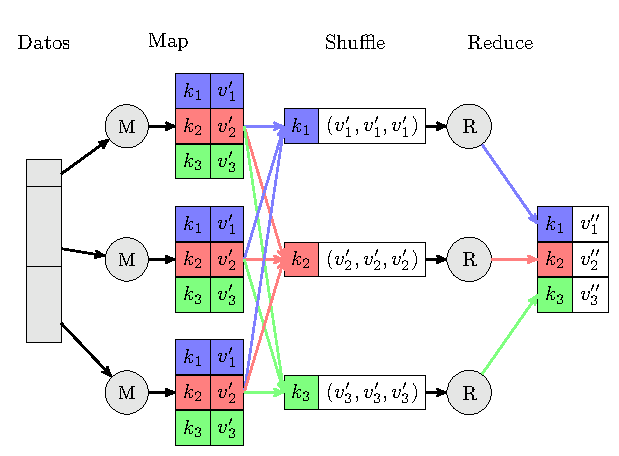
\includegraphics[width=0.8\linewidth]{./Figures/mapreduce.pdf}
	\caption[Esquema de trabajo del paradigma MapReduce.]{Esquema de trabajo del paradigma MapReduce. \textit{Fuente: elaboración propia.}}
	\label{fig:mapreduce}
\end{figure}

Sin embargo, uno de los principales inconvenientes de la herramienta Hadoop es su bajo rendimiento en ciertas condiciones, principalmente en entornos iterativos, debido a la sobrecarga de re-ejecutar todo un trabajo completo cuando no es necesario \cite{Lin13}. Por esta razón, se han realizado esfuerzos para el desarrollo de nuevas herramientas basadas en MapReduce que solucionen los problemas que presenta Hadoop. Entre otras, una de las herramientas más populares que soluciona este problema es Apache Spark \cite{Zcddmmfs12}, el cual presenta una mejora significativa de rendimiento con respecto a Hadoop, principalmente en procesos iterativos, gracias a una abstracción de datos denominada \ac{RDD}. Los RDD se caracterizan por poseer un conjunto de operaciones denominadas transformaciones y acciones, que se basan en un uso intensivo de memoria principal. Asimismo, Spark posee una librería donde los principales algoritmos de minería de datos han sido adaptados para el procesamiento distribuido, denominada MLlib \cite{Mllib15}, junto a un submódulo para el procesamiento por lotes de flujos de datos, denominado Apache Spark Streaming.

En esta tesis doctoral los métodos de extracción de patrones descriptivos se basan en algoritmos evolutivos, los cuales tienen un importante componente iterativo. Por esta razón, el desarrollo de estos métodos complejos se desarrollarán para la herramienta Apache Spark.

\subsection{Minería de flujo de datos} \label{sec:ds}

La cantidad de datos que se generan y no se almacenan es de dos órdenes de magnitud superior a la cantidad de datos que finalmente se almacena, de acuerdo al informe de Cisco mencionado en el apartado anterior. Esto supone que la mayoría de datos generados tiene un carácter efímero y que su interés es relevante hasta unos instantes después de su generación, para ser posteriormente desechados. Esta información, generada principalmente por la alta conectividad entre dispositivos y personas, y el \ac{IoT}, contiene un conocimiento que es interesante para la mejora a corto y largo plazo de la calidad de los procesos, servicios o mejora del bienestar de las personas. A todos estos datos efímeros y generados constantemente se les denomina flujos de datos. Analizar estos flujos de datos es uno de los retos más relevantes de la minería de datos actual, no sólo por sus características, que se detallarán más adelante, sino por la necesidad de crear sistemas que integren los datos provenientes de diferentes fuentes para realizar un análisis eficiente de los mismos.

Un flujo de datos se define como una secuencia potencialmente infinita de instancias, que llegan al sistema a lo largo del tiempo, a una velocidad que puede ser variable \cite{Gaber12}. Estas características suponen una gran diferencia respecto a la minería de datos tradicional. Las más relevantes son \cite{Bifet09Thesis,Gama10}:

\begin{itemize}
	\item No es posible almacenar la totalidad del flujo de datos al ser potencialmente infinito. Por lo que únicamente se pueden almacenar de manera temporal, limitando así la cantidad de veces que puede ser procesado un dato. Normalmente se limita a una única visualización y, tras procesarlo, se descarta.
	
	\item Las instancias no están disponibles para el sistema en su totalidad de antemano, sino que estas llegan al sistema a lo largo del tiempo de manera secuencial o mediante bloques o conjuntos de datos ordenados. De hecho, habitualmente este orden implica cierta dependencia entre un dato y el siguiente.
	
	\item Se asume que la velocidad de llegada de datos es muy alta con respecto a la capacidad de procesamiento del sistema. Por lo tanto, los métodos deben dar respuesta inmediata con el objetivo de evitar demoras y comprometer la estabilidad del sistema.
	
	\item Las características estadísticas de los datos que llegan al sistema pueden evolucionar a lo largo del tiempo, haciendo que los modelos aprendidos no sean válidos. A este proceso se le denomina en la literatura como cambio de concepto \cite{Kshg18}.
\end{itemize}

Con estas características, una mayoría amplia de algoritmos tradicionales de minería de datos no son válidos para el tratamiento de flujos de datos. Esto se debe a que asumen la disponibilidad de la totalidad de los datos, tienen un tiempo de cómputo excesivo o no asumen la variabilidad en la distribución estadística de los datos a lo largo del tiempo, también denominado como cambio de concepto.

El cambio de concepto es uno de los factores más analizados en la literatura especializada en minería de flujo de datos. Este fenómeno se define como cambios en la distribución que subyace en los datos a lo largo del tiempo. La presencia de este tipo de cambio supone que las propiedades aprendidas por un algoritmo de minería de datos se degradan cuando este se produce. En muchos casos, el cambio es lo suficientemente grande como para que la aplicación del modelo no tenga sentido pues su calidad se ha degradado significativamente. Por lo tanto, aplicar técnicas de detección y manejo de cambio de concepto es fundamental para un correcto análisis de los flujos de datos. 



Hay varios aspectos inherentes al cambio de concepto que son necesarios tener en cuenta cuando se analiza su naturaleza \cite{Kshg18}:

\begin{itemize}
	\item Tipo de cambio. En este aspecto, se pueden dar dos tipos de cambio de concepto principales, representados gráficamente en la \Cref{fig:CDTypes}:
	
	\begin{itemize}
		\item Cambio de concepto real. Ocurre cuando se produce un cambio en la probabilidad a posteriori de la clase del patrón $X$, es decir $P\left(v_c|X\right)$. Esta definición, llevada al ámbito \ac{SDRD} y a la nomenclatura utilizada en la Tabla \ref{tab:tablaContingencia}, implica que $P\left(v_c|X\right) = \frac{P(v_cX)}{P(X)} = \frac{tp}{tp+fp} = Conf(X)$.
		Esto afecta por tanto a la frontera de decisión de los modelos pues ha habido una modificación en la distribución que subyace en los datos lo suficientemente grande como para que ya no sean válidas. Por tanto, la confianza (\Cref{eq:conf}) de un patrón se ve alterada en este tipo de cambio de concepto.
		
		\item Cambio de concepto virtual. Se produce cuando cambia la probabilidad condicional de la clase $P\left(X|v_c\right)$, sin afectar a la probabilidad a posteriori $P\left(v_c|X\right)$. Esto implica que la distribución de los datos ha cambiado, pero la frontera de decisión no, por lo que el modelo seguiría siendo válido. Siguiendo la nomenclatura de la Tabla \ref{tab:tablaContingencia}, $P\left(X|v_c\right) = \frac{P(v_cX)}{P(v_c)} = \frac{tp}{tp+fn} = TPR(X)$ . No obstante, este tipo de cambio de concepto es interesante en tareas descriptivas como \ac{SDRD} pues se puede describir un suceso que ha modificado el comportamiento de los datos.
		
\end{itemize}

\begin{figure}[!hbtp]
	\centering
	\subfloat[Datos originales.]{
		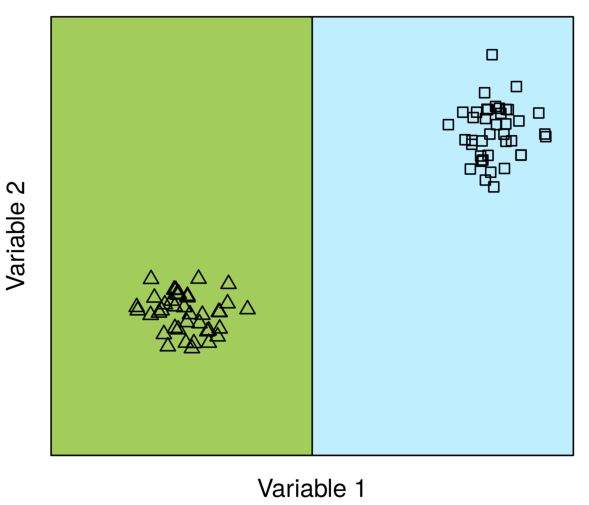
\includegraphics[width=0.3\linewidth]{./Figures/CD_original.pdf}
		\label{fig:CDOriginal}
	}
	\subfloat[Cambio real.]{
		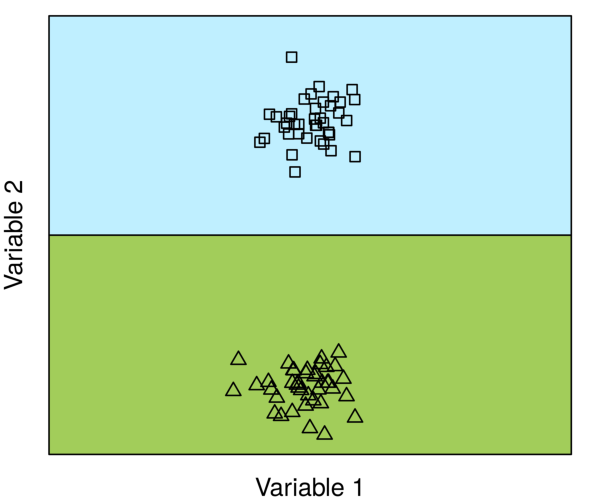
\includegraphics[width=0.3\linewidth]{./Figures/CD_real.pdf}
		\label{fig:CDReal}
	}
	\subfloat[Cambio virtual.]{
		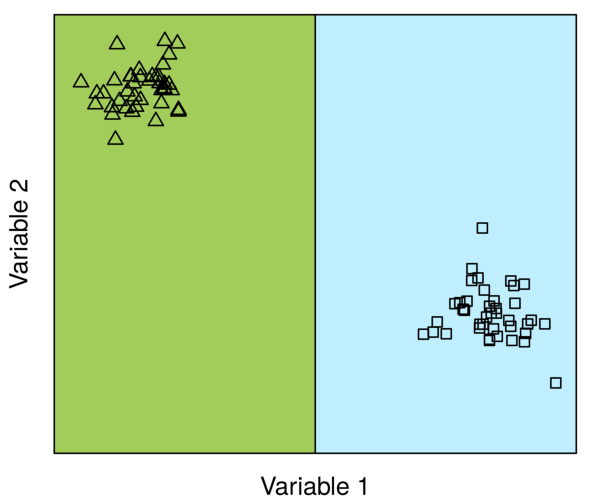
\includegraphics[width=0.3\linewidth]{./Figures/CD_virtual.pdf}
		\label{fig:CDVirtual}
	}
	\caption[Tipos principales de cambio de concepto]{Tipos principales de cambio de concepto en función de su influencia en las fronteras de decisión del modelo. \textit{Fuente: elaboración propia a partir de \cite{Rkgwh17}.}}
	\label{fig:CDTypes}
\end{figure}


	\item Velocidad. En este punto se distingue entre cambios súbitos, es decir, que ocurren abruptamente de una instancia o bloque al siguiente o aquellos que se producen de manera gradual con mayor o menor velocidad a lo largo de una serie de instancias. Al primer tipo de cambio se lo conoce en la literatura como cambio abrupto, mientras que el segundo es conocido como cambio gradual. Un ejemplo ilustrativo de ambos tipos de cambio se muestra en la \Cref{fig:velocidadCambio}.
	
\begin{figure}[!hbtp]
	\centering
	\subfloat[Cambio abrupto.]{
		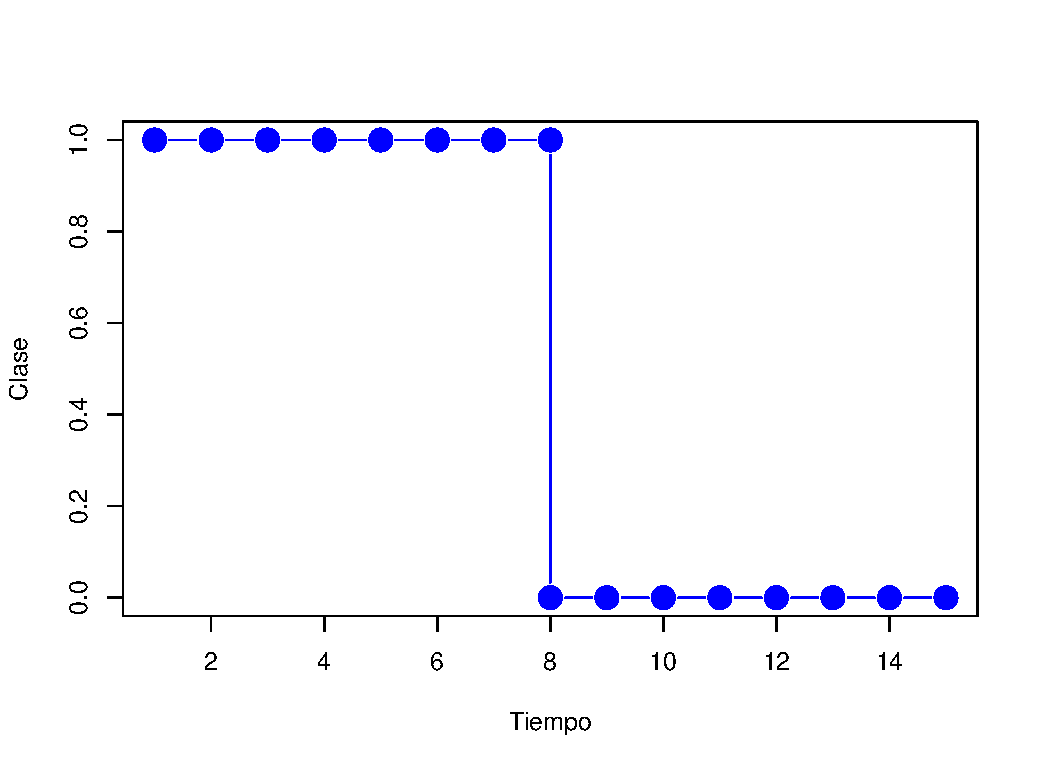
\includegraphics[width=0.5\linewidth]{./Figures/Abrupto.pdf}
		\label{fig:CDAbrupto}
	}
	\subfloat[Cambio gradual.]{
		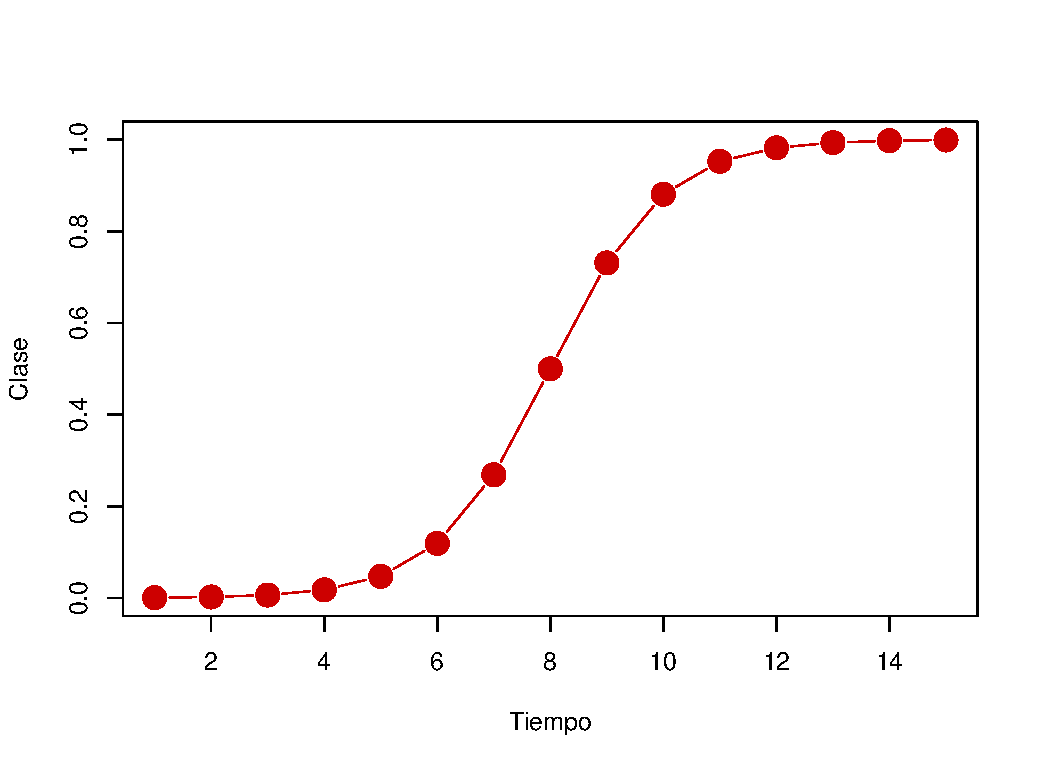
\includegraphics[width=0.5\linewidth]{./Figures/Gradual.pdf}
		\label{fig:CDGradual}
	}
	\caption[Velocidad del cambio de concepto]{Velocidad del cambio de concepto. \textit{Fuente: elaboración propia a partir de \cite{Rkgwh17}.}}
	\label{fig:velocidadCambio}
\end{figure}
	
	\item Severidad. Un cambio de concepto puede afectar a una zona reducida del espacio de búsqueda, denominado cambio local, o puede afectar a todo el espacio de búsqueda, siendo así un cambio global. Un ejemplo ilustrativo de ambos tipos de cambio se muestra en la \Cref{fig:severidadCambio}.
	
	\begin{figure}[!hbtp]
		\centering
		\subfloat[Datos originales.]{
			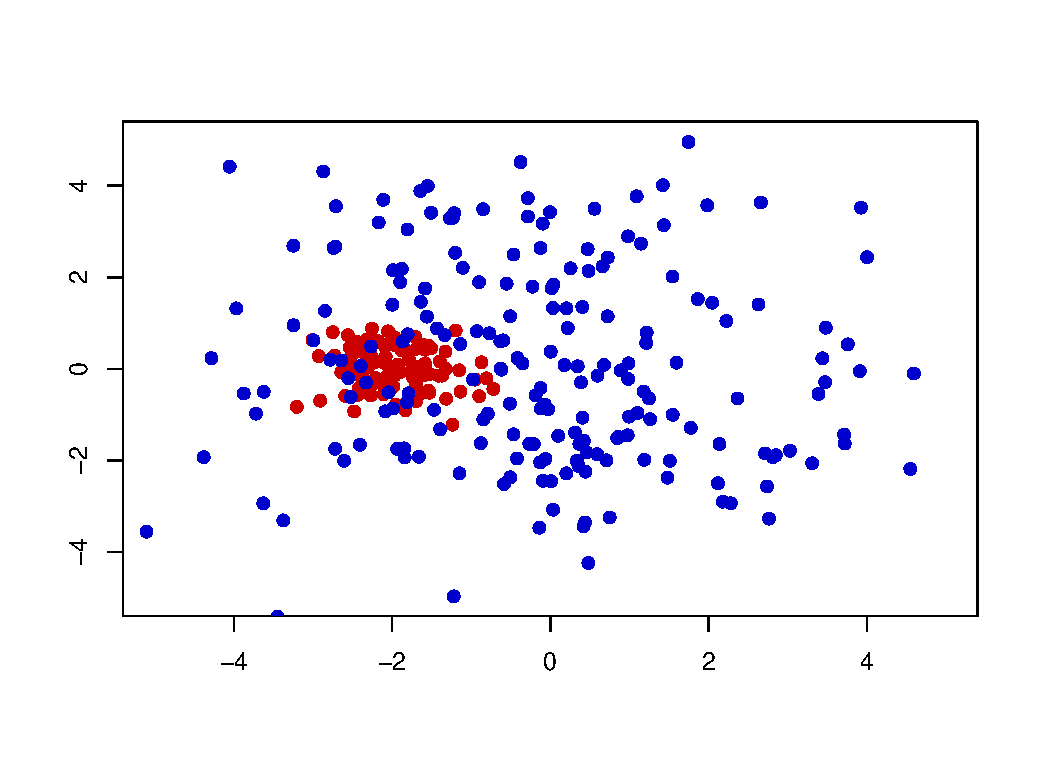
\includegraphics[width=0.3\linewidth]{./Figures/SeverityOriginal.pdf}
			\label{fig:SeverityOriginal}
		}
		\subfloat[Cambio Global.]{
			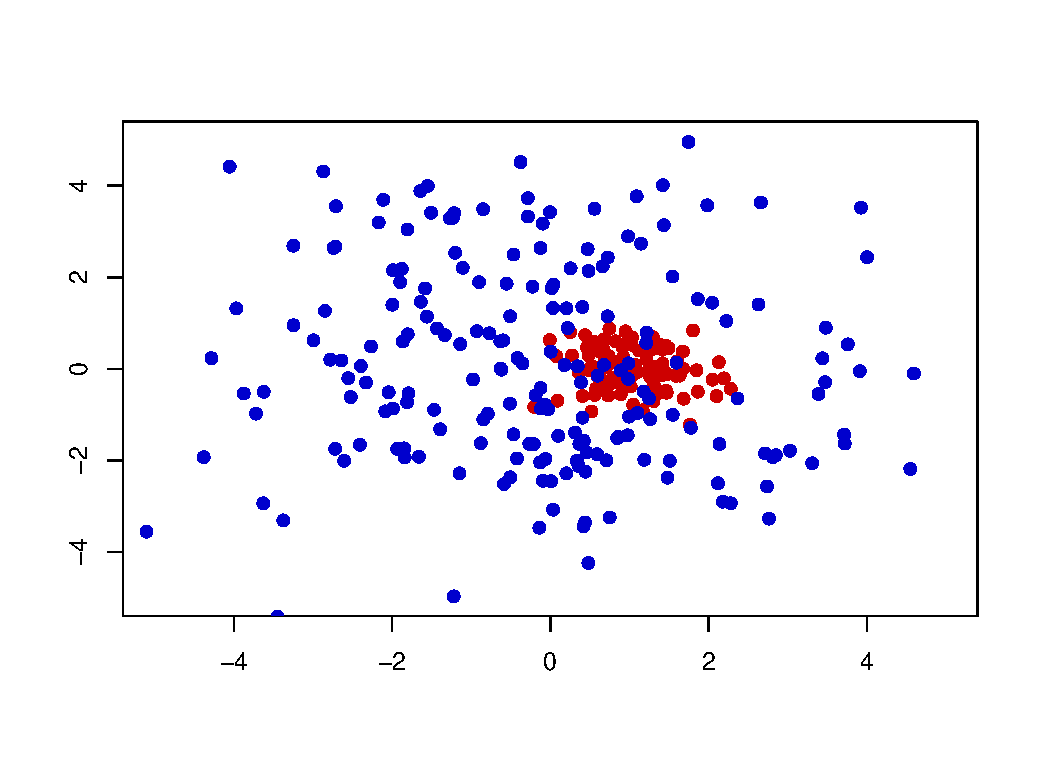
\includegraphics[width=0.3\linewidth]{./Figures/SeverityGlobal.pdf}
			\label{fig:SeverityGlobal}
		}
		\subfloat[Cambio Local.]{
			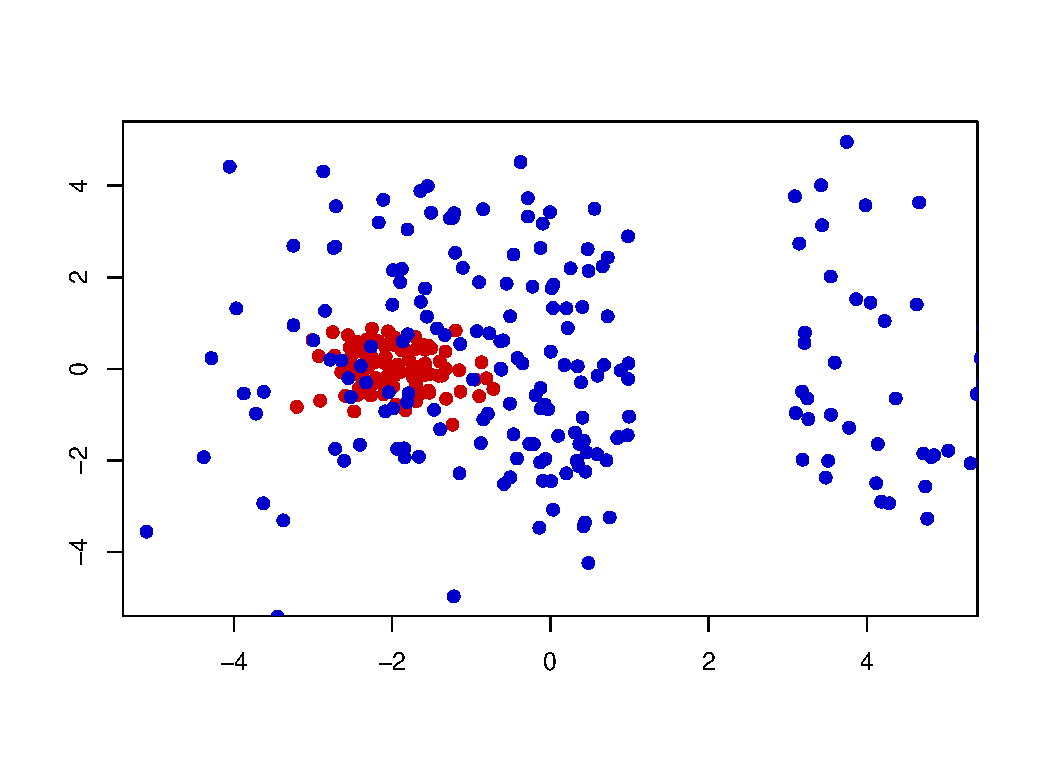
\includegraphics[width=0.3\linewidth]{./Figures/SeverityLocal.pdf}
			\label{fig:SeverityLocal}
		}
		\caption[Severidad del cambio de concepto]{Severidad del cambio de concepto. \textit{Fuente: elaboración propia a partir de \cite{Kshg18}.}}
		\label{fig:severidadCambio}
	\end{figure}
	
	\item Recurrencia. Un concepto puede ser cíclico si a intervalos regulares se produce el cambio, como por ejemplo aquellas aplicaciones sujetas a variaciones estacionales, o bien pueden ser cambios acíclos, cuando se desconoce la repetición del concepto. Un ejemplo ilustrativo de ambos tipos de cambio se muestra en la \Cref{fig:recurrenciaCambio}.
	
	\begin{figure}[!hbtp]
		\centering
		\subfloat[Cambio cíclico.]{
			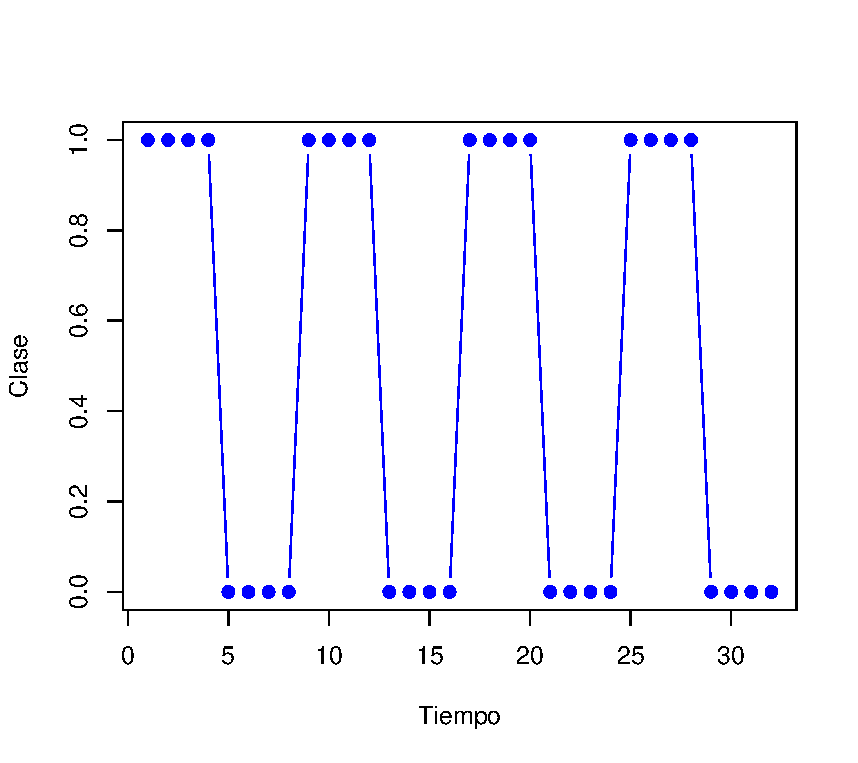
\includegraphics[width=0.5\linewidth]{./Figures/CambioRecurrente.pdf}
			\label{fig:cambioCiclico}
		}
		\subfloat[Cambio acíclico.]{
			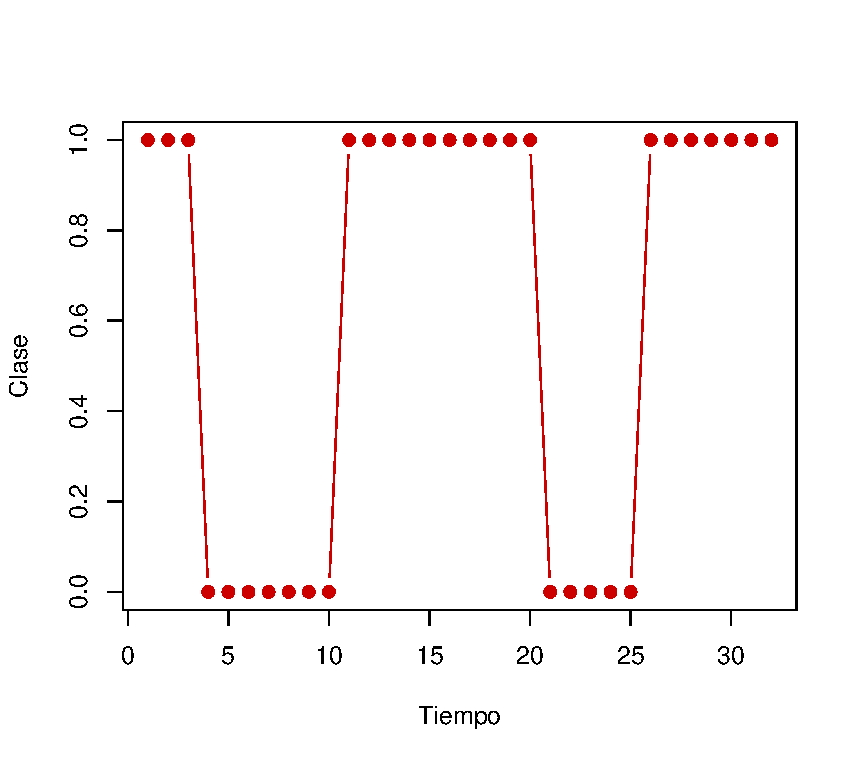
\includegraphics[width=0.5\linewidth]{./Figures/CambioAciclico.pdf}
			\label{fig:cambioAclico}
		}
		\caption[Recurrencia del cambio de concepto]{Recurrencia del cambio de concepto. \textit{Fuente: elaboración propia a partir de \cite{Rkgwh17}.}}
		\label{fig:recurrenciaCambio}
	\end{figure}
\end{itemize}

Para gestionar el cambio de concepto, a lo largo de la literatura se han empleado tres enfoques diferentes \cite{Rkgwh17}: 

\begin{itemize}
	\item Entrenar el modelo desde cero cada vez que llegue una nueva instancia o bloque de datos. Este enfoque tiene un alto coste computacional y es inviable en la mayoría de escenarios \cite{Kj00,Sk01,Zmlr04}.
	
	\item Entrenar el modelo desde cero cuando se detecte un cambio de concepto. Para ello, se utilizan detectores de cambio de concepto que pueden ser dependientes o no del modelo de aprendizaje. Estos sistemas mandan una señal de alerta e informan sobre la severidad del cambio al algoritmo de aprendizaje. Este punto de vista permite aligerar la carga computacional siempre y cuando el entorno no sea altamente cambiante \cite{Gmcr04, Bg07,Pw13,Vm14}.
	
	\item Usar un método de aprendizaje adaptativo que permite seguir el estado del flujo de datos y adaptarse automáticamente al mismo. En este punto, existen diferentes enfoques que se han utilizado a lo largo de la literatura, entre los que destacan:
	
	\begin{itemize}
		\item Ventanas deslizantes. Se define como una o varias memorias que almacenan los datos más recientes, o resúmenes sobre los mismos, que pertenecen al concepto actual. Ha sido uno de los métodos más utilizados a lo largo de la literatura gracias a su versatilidad y bajo consumo de recursos \cite{Wk96,Hsd01, Bbdmw02,Gc06,Ks14,Tran19}. 
		
		\item Métodos \textit{online}. Estos métodos actualizan el modelo instancia a instancia, por lo que son capaces de adaptarse a los cambios tan pronto como ocurren. Es importante destacar que algunos métodos de clasificación como las redes neuronales o Naïve Bayes pueden funcionar de esta manera. Sin embargo, diseñar este tipo de métodos es complejo.
		
		\item Uso de \textit{ensembles}. Aglutina diferentes métodos de aprendizaje de modo que pueden adaptarse sencillamente modificando la estructura de los diferentes algoritmos de los que se compone. Esto permite ganancias tanto en calidad como en flexibilidad \cite{Kmgsw17}.
	\end{itemize}
\end{itemize}

Actualmente existe un gran interés por la minería de flujos de datos. Esto se observa en el número de trabajos que han aparecido recientemente, en donde se pueden encontrar trabajos para tareas de reglas de asociación \cite{Rc18}, mediante \textit{ensembles} \cite{Rlzlll18,soares2018,junior2019}, \textit{deep learning} \cite{Mjsgvr18}, \textit{big bata} \cite{Lsdych17,Fmc18}, aplicaciones \cite{Cstbpgfgd18,Khlm18}, entre otros.

Sin embargo, dentro de la comunidad investigadora aún no se han propuesto métodos para aprovechar el potencial que posee \ac{SDRD} en general, y en especial \ac{EPM}, a los flujos continuos de datos. En esta tesis se propone el desarrollo de sistemas difusos evolutivos capaces de extraer patrones emergentes en flujos continuos de datos para explicar el fenómeno que subyace en los mismos. El reto en este aspecto es afrontar los problemas de dimensionalidad, variedad y carácter dinámico de los datos, haciendo especial hincapié en la necesidad de abordar correctamente la evolución de los conceptos.

\clearpage{} \cleardoublepage
\clearpage{}\acused{SDRD}
\chapter{Discusión de los resultados} \label{chap:discusion}

En este capítulo se resumen las propuestas llevadas a cabo para satisfacer los objetivos planteados en el capítulo introductorio. Para cada uno de los diferentes trabajos presentados en esta memoria, se muestra un breve resumen de las principales ideas propuestas, así como una discusión de los resultados obtenidos. La investigación realizada para esta tesis doctoral y los resultados asociados se agrupan en las siguientes publicaciones en revistas internacionales indexadas en \ac{JCR}:
\begin{itemize}
	\item Trabajos relacionados con \ac{SD}:
	
	\begin{itemize}
		\item \fullcite{Lgpc16}. DOI: 10.1007/s00500-016-2300-1, IF (JCR 2016): 2.472, Ranking: 33/105 (Computer Science, Interdisciplinary Applications), Cuartil: Q2.
		
		\item \fullcite{Gcgcd16}. DOI: 10.32614/RJ-2016-048, IF (JCR 2016): 1.075, Ranking: 55/124 (Statistics \& Probability), Cuartil: Q2.
		
		\item \fullcite{Lcgjv19}. DOI: 10.2991/ijcis.d.191213.001, IF (JCR 2018): 2.153, Ranking: 55/106 (Computer Science, Interdisciplinary Applications), Cuartil: Q3.
		
	\end{itemize}
	
	\item Trabajos relacionados con \ac{EPM}:
	
	\begin{itemize}
	\item \fullcite{Gcmgj18}. DOI: 10.1002/widm.1231, IF (JCR 2018): 2.541, Ranking: 26/105 (Computer Science, Theory \& Methods), Cuartil: Q1.
	
	\item \sloppy \fullcite{Gcgd18}. DOI: 10.1109/TFUZZ.2018.2814577, IF (JCR 2018): 8.759, Ranking: 6/134 (Computer Science, Artificial Intelligence), Cuartil: Q1.
	


	\item \fullcite{Gcgd19}. DOI: 10.1007/s12559-018-9612-7, IF (JCR 2018): 4.287, Ranking: 25/134 (Computer Science, Artificial Intelligence), Cuartil: Q1.
	


	\item \fullcite{Gcgd19a}. DOI: No disponible, IF (JCR 2018): 8.759, Ranking: 6/134 (Computer Science, Artificial Intelligence), Cuartil: Q1.
	\end{itemize}
	
\end{itemize}

Este capítulo se organiza de la siguiente manera: En primer lugar, el \Cref{sec:ruido} presenta un estudio sobre la influencia del ruido en los sistemas difusos evolutivos desarrollados para \ac{SD}. A continuación, el \Cref{sec:paqueteR} muestra las ideas principales del desarrollo de un paquete para la herramienta R que contiene los principales sistemas difusos evolutivos para \ac{SD}. En el \Cref{sec:MIL} se realiza un análisis sobre el comportamiento de los principales enfoques para \ac{SD} en problemas de aprendizaje multi-instancia. Después, el \Cref{sec:reviewEPM} presenta una revisión bibliográfica sobre la \ac{EPM} desde el punto de vista descriptivo. Tras esto, se desarrolla un nuevo sistema difuso evolutivo para la extracción de patrones emergentes descriptivos en el \Cref{sec:moea-efep}. A continuación, se propone un nuevo enfoque evolutivo para la extracción de patrones emergentes en entornos \textit{big data} en el \Cref{sec:bd-efep}. Finalmente, esta tesis doctoral se cierra con el desarrollo de un nuevo sistema difuso evolutivo para la extracción de patrones emergentes en flujos continuos de datos en el \Cref{sec:streaming}.


\section{Influencia del ruido en sistemas difusos evolutivos para descubrimiento de subgrupos} \label{sec:ruido}

En la mayoría de aplicaciones reales existen corrupciones de datos que perjudican el análisis, la interpretación y las decisiones tomadas a partir de los modelos obtenidos de estos datos. Estas alteraciones, conocidas como ruido, son especialmente graves en problemas supervisados ya que se desfigura la relación que existe entre la entrada y la salida del sistema. Por lo tanto, en la literatura existe un gran interés por la detección y tratamiento del ruido en problemas de clasificación y regresión \cite{garcia2015}. Como \ac{SD} es una tarea que utiliza aprendizaje supervisado, el efecto negativo de este ruido puede producirse. Sin embargo, en aplicaciones descriptivas este problema no ha sido estudiado en profundidad. En este trabajo se analiza el efecto del ruido en los algoritmos basados en sistemas difusos evolutivos para \ac{SD} y cómo se pueden aliviar los efectos del mismo utilizando los enfoques de manejo del ruido más apropiados.

En concreto, uno de los enfoques más populares es el empleo de filtros \cite{Brodley99identifyingmislabeled,Khoshgoftaar07ImprovingSoftware} ya que estos actúan como una fase de preprocesamiento eliminando aquellas instancias identificadas como ruido. Por lo tanto, el algoritmo original no necesita ser modificado. Este hecho, que es especialmente relevante para clasificación o regresión, no está claro en \ac{SD} pues aún no se ha analizado en profundidad el efecto de la eliminación de instancias con las métricas que se emplean en \ac{SDRD}.

El estudio experimental se realizó sobre una batería de 37 conjuntos de datos del repositorio de datos de KEEL\footnote{\url{https://sci2s.ugr.es/keel/datasets.php}}. A estos datos, se les introdujo ruido sobre la variable objetivo de manera de artificial utilizando el método \textit{uniform} \cite{Teng99CorrectingNoisy}. Siguiendo este proceso, se crearon diferentes niveles de ruido: 0\%, 5\%, 10\%, 15\% y 20\%, para determinar la influencia del mismo en los algoritmos.

Los algoritmos de \ac{SD} utilizados fueron SDIGA, NMEEFSD y FuGePSD. Es importante destacar que todos ellos son sistemas difusos evolutivos, ya que el objetivo de este trabajo consiste en comprobar la robustez de los sistemas basados en lógica difusa y cómo son capaces de recuperarse en entornos con ruido.  Por su parte, los filtros de ruido empleados fueron: \textit{ensemble filter} \cite{Brodley99identifyingmislabeled}, \textit{cross-validated committees filter} \cite{Verbaeten03EnsembleMethods} e \textit{iterative-partitioning filter} \cite{Khoshgoftaar07ImprovingSoftware}. En este estudio la calidad de las reglas se midió desde tres perspectivas diferentes: interés, mediante la métrica \ac{WRAcc}; generalidad, usando \ac{TPR}; y fiabilidad, utilizando la medida confianza. Además, se analizó la interpretabilidad de los modelos extraídos en función del número de patrones y variables. Los resultados fueron comparados entre sí utilizando pruebas estadísticas. 

De acuerdo a los resultados extraídos en la experimentación, se observa que el ruido en este tipo de algoritmos influye de manera negativa en los resultados obtenidos a pesar de la robustez que proporciona la lógica difusa en este tipo de escenarios. No obstante, esta influencia se puede mitigar empleando algoritmos de filtrado de ruido. De acuerdo a los resultados, el \textit{ensemble filter} reporta mejoras en la calidad de los algoritmos de \ac{SD} en todos los aspectos que se han analizado. Por lo tanto, es interesante que se aplique este tipo de algoritmos como preprocesamiento en aplicaciones reales. En contraposición, se destaca que el algoritmo FuGePSD es capaz de detectar el ruido y aislarlo, de modo que no es necesario la aplicación de ningún tipo de filtro adicional. Esto abre la posibilidad de continuar en la línea de desarrollo de métodos robustos frente a ruido.

En cuanto a la interpretabilidad de los modelos, de este estudio se extrae que la aplicación de filtros de ruido mejora ligeramente la interpretabilidad de los mismos. Se destaca además que la aplicación de estos filtros parece tener una mayor mejora en aquellos algoritmos que tienen propensión a obtener modelos con muchos patrones simples, es decir, con pocas variables. Esto se debe a la eliminación de instancias en las fronteras entre clases, permitiendo así una mejor detección mediante patrones simples.


Como conclusión final de este trabajo, se destaca la necesidad de seguir investigando en esta línea de trabajo desde el desarrollo de nuevos métodos robustos frente a ruido, así como en la creación de técnicas de preprocesamiento enfocadas al tratamiento de ruido específicas para \ac{SD}.

El trabajo de investigación asociado a esta parte es:

\begin{itemize}
	\item \fullcite{Lgpc16}. \\DOI: \doi{10.1007/s00500-016-2300-1}, IF (JCR 2016): 2.472, Ranking: 33/105 (Computer Science, Interdisciplinary Applications), Cuartil: Q2.
\end{itemize}

\section{Descubrimiento de subgrupos con sistemas difusos evolutivos en R: el paquete SDEFSR} \label{sec:paqueteR}

A día de hoy, existen para \ac{SD} varias herramientas disponibles para el empleo de los algoritmos más destacados de la literatura. El software más conocido actualmente que contienen paquetes de algoritmos de \ac{SD} son KEEL \cite{KEEL3}, VIKAMINE \cite{Al12}, ORANGE \cite{Orange} y CORTANA \cite{Kl11}.

R\footnote{\url{https://cran.r-project.org/}} es un lenguaje de programación bajo licencia GNU para computación estadística y generación de gráficas que provee una amplia variedad de funcionalidades estadísticas, así como una amplia variedad de algoritmos de la mayoría de campos de la minería de datos actual. R se podría considerar a día de hoy como una de las aplicaciones software más potentes para el análisis y visualización de datos. Uno de los principales causantes de su éxito es la posibilidad de ampliar su funcionalidad a través de paquetes software que la comunidad crea y distribuye libremente. 

A pesar de su éxito, en R únicamente existe un paquete relacionado con métodos de \ac{SD}, denominado \textit{rsubgroup}\footnote{\url{http://www.rsubgroup.org/}}. Este paquete se trata de una interfaz para R del programa VIKAMINE, el cual contiene algoritmos de \ac{SD} con enfoques clásicos. Por lo tanto, era necesario llevar a esta herramienta aquellos algoritmos de \ac{SD} basados en sistemas difusos evolutivos más relevantes debido a la calidad del conocimiento que extraen \cite{Cgdh14}.

Para ello, se ha realizado un paquete para el software R denominado SDEFSR\footnote{\url{https://cran.r-project.org/web/packages/SDEFSR/index.html}} (\textit{Subgroup Discovery with Evolutionary Fuzzy Systems for R}). En este paquete se han implementado cuatro algoritmos de \ac{SD} basados en sistemas difusos evolutivos: SDIGA \cite{Dghm07}, MESDIF \cite{Dgh07}, NMEEF-SD \cite{Cgdh10} y FuGePSD \cite{Crdwgge15}. Estos algoritmos son totalmente configurables, aunque se proponen valores por defecto para facilitar su uso. El objetivo es proveer a la comunidad de R con los algoritmos basados en sistemas difusos evolutivos para \ac{SD} más relevantes de la literatura. 

Los algoritmos incluidos en este paquete son capaces de leer datos desde diferentes formatos: ARFF, de la herramienta Weka \cite{Weka2009}, CSV, KEEL, así como desde la estructura de datos \textit{data.frame} propia de R, permitiendo ampliar el espectro de formatos utilizando paquetes externos a SDEFSR.

Tras la ejecución de un método de \ac{SD} en SDEFSR, se puede realizar un análisis y post-procesamiento de los resultados obtenidos. Esto es posible gracias a que el paquete proporciona una utilidad para visualizar los patrones en un gráfico mostrando su calidad respecto a las medidas \ac{TPR} y \ac{FPR} para determinar su fiabilidad y generalidad. Asimismo, el paquete aporta la funcionalidad suficiente para realizar operaciones básicas de post-procesamiento, como el filtrado por una medida de calidad o número de reglas de manera sencilla.




Finalmente, el paquete SDEFSR incluye una aplicación web que permite realizar todo el procedimiento de \ac{SD}, así como una visualización básica de datos de manera gráfica. Un ejemplo de este interfaz se puede observar en la \Cref{fig:webSDR}. El objetivo es acercar toda la funcionalidad que ofrece este paquete a aquellas personas con muy poca experiencia de programación, o aquellas que prefieren hacer el proceso de manera gráfica. 

\begin{figure}[!hbtp]
	\centering
	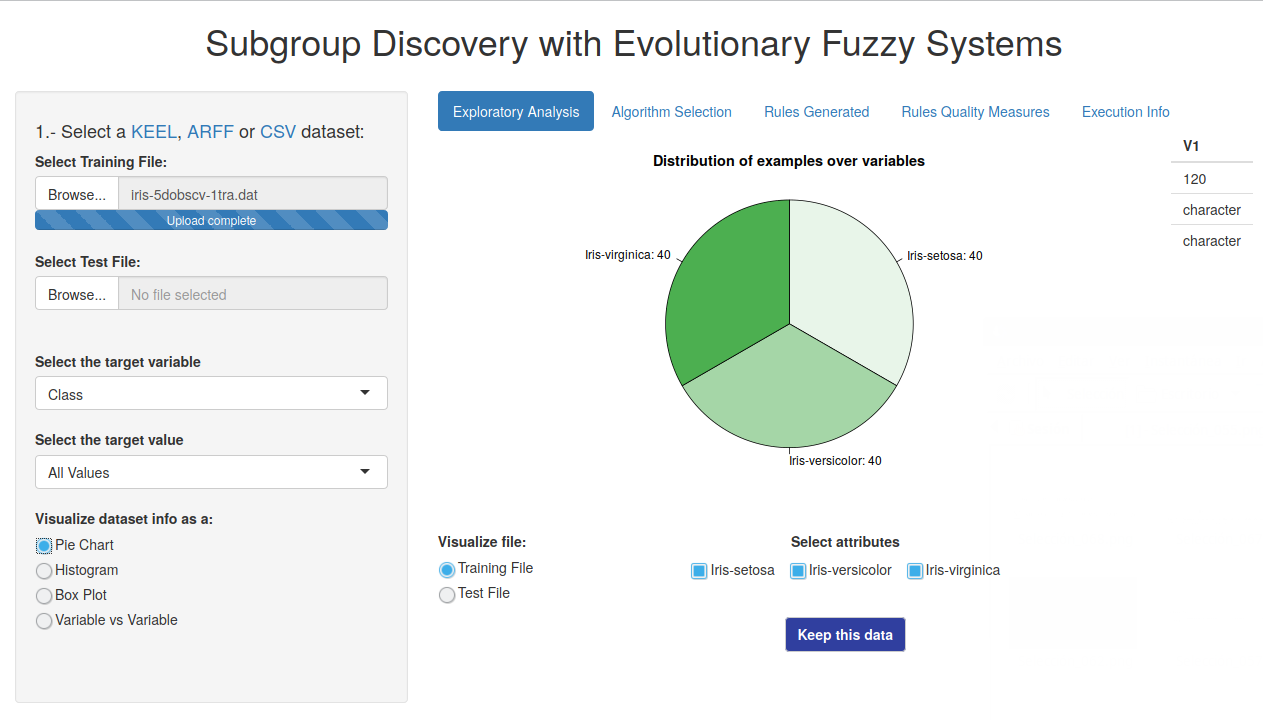
\includegraphics[width=0.8\linewidth]{./Figures/SDEFSR_GUI.png}
	\caption[Ejemplo de la interfaz web para el empleo del paquete SDEFSR]{Ejemplo de la interfaz web para el empleo del paquete SDEFSR. Detalle del empleo del visualizador básico de datos. \textit{Fuente: elaboración propia.}}
	\label{fig:webSDR}
\end{figure}

A fecha de hoy, el impacto del paquete en la comunidad de R es aceptable, con un total de 5382 descargas\footnote{\url{https://cranlogs.r-pkg.org/badges/grand-total/SDEFSR}} desde su lanzamiento en 2016. Actualmente se sigue trabajando activamente en la mejora del mismo, ampliando su funcionalidad y mejorando la eficiencia para producir un mayor impacto en la comunidad de R.


Como conclusión final, se destaca que el estudio de métodos y herramientas, junto al desarrollo de este paquete software, ha permitido realizar una profunda revisión bibliográfica sobre la tarea. Esta revisión ha permitido identificar las diferentes propuestas publicadas y conocer sus limitaciones, permitiendo detectar problemas abiertos para trabajos de investigación futuros.

El trabajo de investigación asociado a esta parte es:

\begin{itemize}
	\item \fullcite{Gcgcd16}. DOI: \doi{10.32614/RJ-2016-048}, IF (JCR 2016): 1.075, Ranking: 55/124 (Statistics \& Probability), Cuartil: Q2. 

\item \fullcite{Gcgcj15}.
\end{itemize}



\section{Análisis de los principales enfoques para descubrimiento de subgrupos en problemas de aprendizaje multi-instancia} \label{sec:MIL}

Debido a la creciente demanda de almacenamiento, a día de hoy el almacenaje de los mismos se realiza de muy diversas maneras. Una de ellas es la de agrupar varias instancias que de alguna manera se encuentran relacionadas por la misma causa en bolsas. Usando esta representación, conocida en la literatura como multi-instancia \cite{HerreraVBCZSV16}, la variable objetivo se asocia directamente con la bolsa de instancias y no con cada una de las instancias individuales que la conforman. Este tipo de problemas han sido ampliamente estudiados por la comunidad de aprendizaje supervisado, en especial para problemas de clasificación debido a su utilidad \cite{Amores13}. Sin embargo, como resultado del trabajo de revisión realizado anteriormente, se descubrió que no existe ningún algoritmo específicamente desarrollado para la tarea de \ac{SD} enfocado a resolver problemas \ac{MIL}. 

Por lo tanto, el objetivo de este trabajo es una primera aproximación a los problemas \ac{MIL} en \ac{SD}. Para ello, se realiza una adaptación de los enfoques más relevantes en \ac{SD} a problemas \ac{MIL}. En concreto, se utiliza un algoritmo exhaustivo, SD-Map \cite{Ap06}, y dos algoritmos no exhaustivos: CGBA-SD \cite{Lrrv14} y NMEEF-SD \cite{Cgdh10}. SD-Map se basa en el conocido algoritmo FP-Growth \cite{han2004mining}, mientras que CGBA-SD se basa en programación genética y NMEEF-SD se basa en un sistema difuso evolutivo multi-objetivo.

En \cite{Amores13} se presenta una revisión de los paradigmas más destacados que se han utilizado en \ac{MIL}. Desde un punto de vista descriptivo, los enfoques basados en el espacio de bolsa o en el espacio embebido no son relevantes pues se pierde la información relacionada con las instancias. Por esta razón, los algoritmos de \ac{SD} se modifican basándose en el paradigma del espacio de instancia. A modo de resumen, la adaptación llevada a cabo en estos algoritmos se encuentra en el conteo de características o instancias cubiertas realizado para el cálculo de las medidas de calidad. En concreto, se emplea la asunción estándar del problema multi-instancia. Por un lado, el conteo de características se incrementará solo una vez por bolsa si dicha característica aparece al menos una vez en la bolsa. Por otro lado, una bolsa será marcada como cubierta por un patrón si al menos una de sus instancias es cubierta.

Del estudio experimental llevado a cabo, se observa que el enfoque exhaustivo produce unos resultados bastante pobres en calidad. Por su parte, CGBA-SD muestra un mejor comportamiento en general, presentando unos resultados de calidad competentes. Finalmente, el algoritmo NMEEF-SD presenta un comportamiento más variado, pues obtiene resultados de baja calidad en problemas de identificación de contenido en imágenes, mientras que en el resto se obtienen unos resultados interesantes y precisos. 

Como conclusión, el trabajo realizado consiste en una primera aproximación a \ac{MIL} de los principales algoritmos de \ac{SD} basados en diferentes enfoques de extracción de patrones. Por tanto, este trabajo aporta a la sociedad una nueva posibilidad de resolución de problemas anteriormente no disponible. Asimismo, el aporte realizado a la comunidad científica en este trabajo destaca por la posibilidad de continuar investigando en esta nueva línea de trabajo tras la obtención de resultados prometedores.



El trabajo de investigación asociado a esta parte es:

\begin{itemize}
	\item \fullcite{Lcgjv19}. DOI: \doi{10.2991/ijcis.d.191213.001}, IF (JCR 2018): 2.153, Ranking: 55/106 (Computer Science, Interdisciplinary Applications), Cuartil: Q3.
\end{itemize}


\section{Revisión de la minería de patrones emergentes desde el punto de vista descriptivo} \label{sec:reviewEPM}

\ac{EPM} tiene como objetivo la búsqueda de patrones discriminatorios cuyo soporte entre diferentes clases o conjuntos de datos difiera de manera significativa \cite{Dl99}. De este modo, se pueden describir las características discriminadoras entre las diferentes clases de un problema o el descubrimiento de tendencias emergentes a lo largo del tiempo. Dado que \ac{EPM} se basa principalmente en el empleo de la medida \ac{GR} (\Cref{eq:gr}), estos poseen un alto poder discriminatorio. Por esta razón, a lo largo de la literatura se han empleado y desarrollado modelos de extracción de patrones únicamente enfocados a maximizar la precisión de los modelos, ignorando en gran medida el carácter descriptivo que poseen los patrones.

En este trabajo se realiza una revisión y análisis de los principales enfoques desarrollados para \ac{EPM} desde el punto de vista descriptivo. Para ello, se analiza el comportamiento de los principales algoritmos desarrollados a lo largo de la literatura. También se analiza la influencia de diferentes mecanismos de filtrado de patrones para la mejora de las capacidades descriptivas de los modelos extraídos. El objetivo es el establecimiento de una línea a seguir para el desarrollo de futuras propuestas enfocadas al aspecto descriptivo.

Fruto del trabajo de revisión realizado, se han identificado tres subconjuntos interesantes de patrones emergentes en función de sus características: patrones minimales y maximales, patrones \textit{jumping} y patrones tolerantes a ruido. Además, se ha llevado a cabo una taxonomía de algoritmos de extracción de patrones emergentes en donde se han identificado cuatro enfoques principales: (1) basados en límites, (2) basados en árboles, (3) basados en árboles de decisión y (4) basados en sistemas difusos evolutivos. Es importante destacar la evolución que han sufrido estos enfoques con respecto a las capacidades descriptivas de los modelos, en donde los primeros enfoques ignoran totalmente el aspecto descriptivo, mientras que el tercer y cuarto enfoque sí lo tienen en cuenta e introducen diversos mecanismos, como el empleo de lógica difusa, entre otros, para mantener cierto nivel de interpretabilidad.

Para la obtención de conclusiones fundamentadas, se ha realizado un estudio experimental con un amplio número de conjuntos de datos, así como el empleo de pruebas estadísticas para determinar el nivel de significación de las diferencias. Este procedimiento se ha llevado a cabo sobre cinco medidas de calidad, permitiendo determinar las características descriptivas de los patrones: fiabilidad, generalidad e interpretabilidad. 

De los resultados obtenidos, se pueden obtener las siguientes conclusiones:

\begin{itemize}
	\item Los patrones tipo Chi son muy interesantes desde el punto de vista descriptivo. Esto se debe principalmente al empleo de un umbral de soporte mínimo junto a la utilización de la prueba $\chi^2$, el cual permite determinar si todos los selectores de un patrón aportan información de manera significativa. Sin embargo, a pesar de sus grandes cualidades, el alto número de restricciones hace que sea muy difícil extraer este tipo de patrón en problemas complejos.
	
	\item El post-procesamiento de los patrones extraídos es necesario en la mayoría de los casos para mejorar las cualidades descriptivas. Por lo tanto, es interesante integrar en futuros desarrollos estos mecanismos para mejorar las cualidades descriptivas. En concreto, se destaca la búsqueda de patrones minimales con altos niveles de confianza. 
	
	\item El empleo de lógica difusa es vital para la mejora de los modelos en el enfoque descriptivo. Su uso permite obtener altos niveles de calidad en todos los aspectos analizados, mejorando la interpretabilidad de los modelos. Por lo tanto, se anima a su empleo para futuros desarrollos.
	
	\item  El enfoque basado en sistemas difusos evolutivos es capaz de obtener unos niveles de calidad desde el punto de vista descriptivo similares a los mejores métodos analizados, con un número de patrones significativamente menor que el resto. Este reciente enfoque de \ac{EPM} es muy interesante desde el punto de vista descriptivo e invita al desarrollo de nuevos algoritmos basados en métodos evolutivos o en otras metaheurísticas.
	
	\item Se identificaron los principales métodos para la extracción de patrones emergentes descriptivos en la literatura basándose en los tres objetivos principales de \ac{SDRD}: precisión, interés y generalidad. El resultado de este estudio, mostrado en la \Cref{fig:friedman} destaca la calidad de los algoritmos FEPM, iEPM y EvAEP, por tanto, es interesante de cara a futuros desarrollos el análisis profundo de estos algoritmos para mejorar sus capacidades descriptivas.
	
	\begin{figure}[!hbtp]
		\centering
		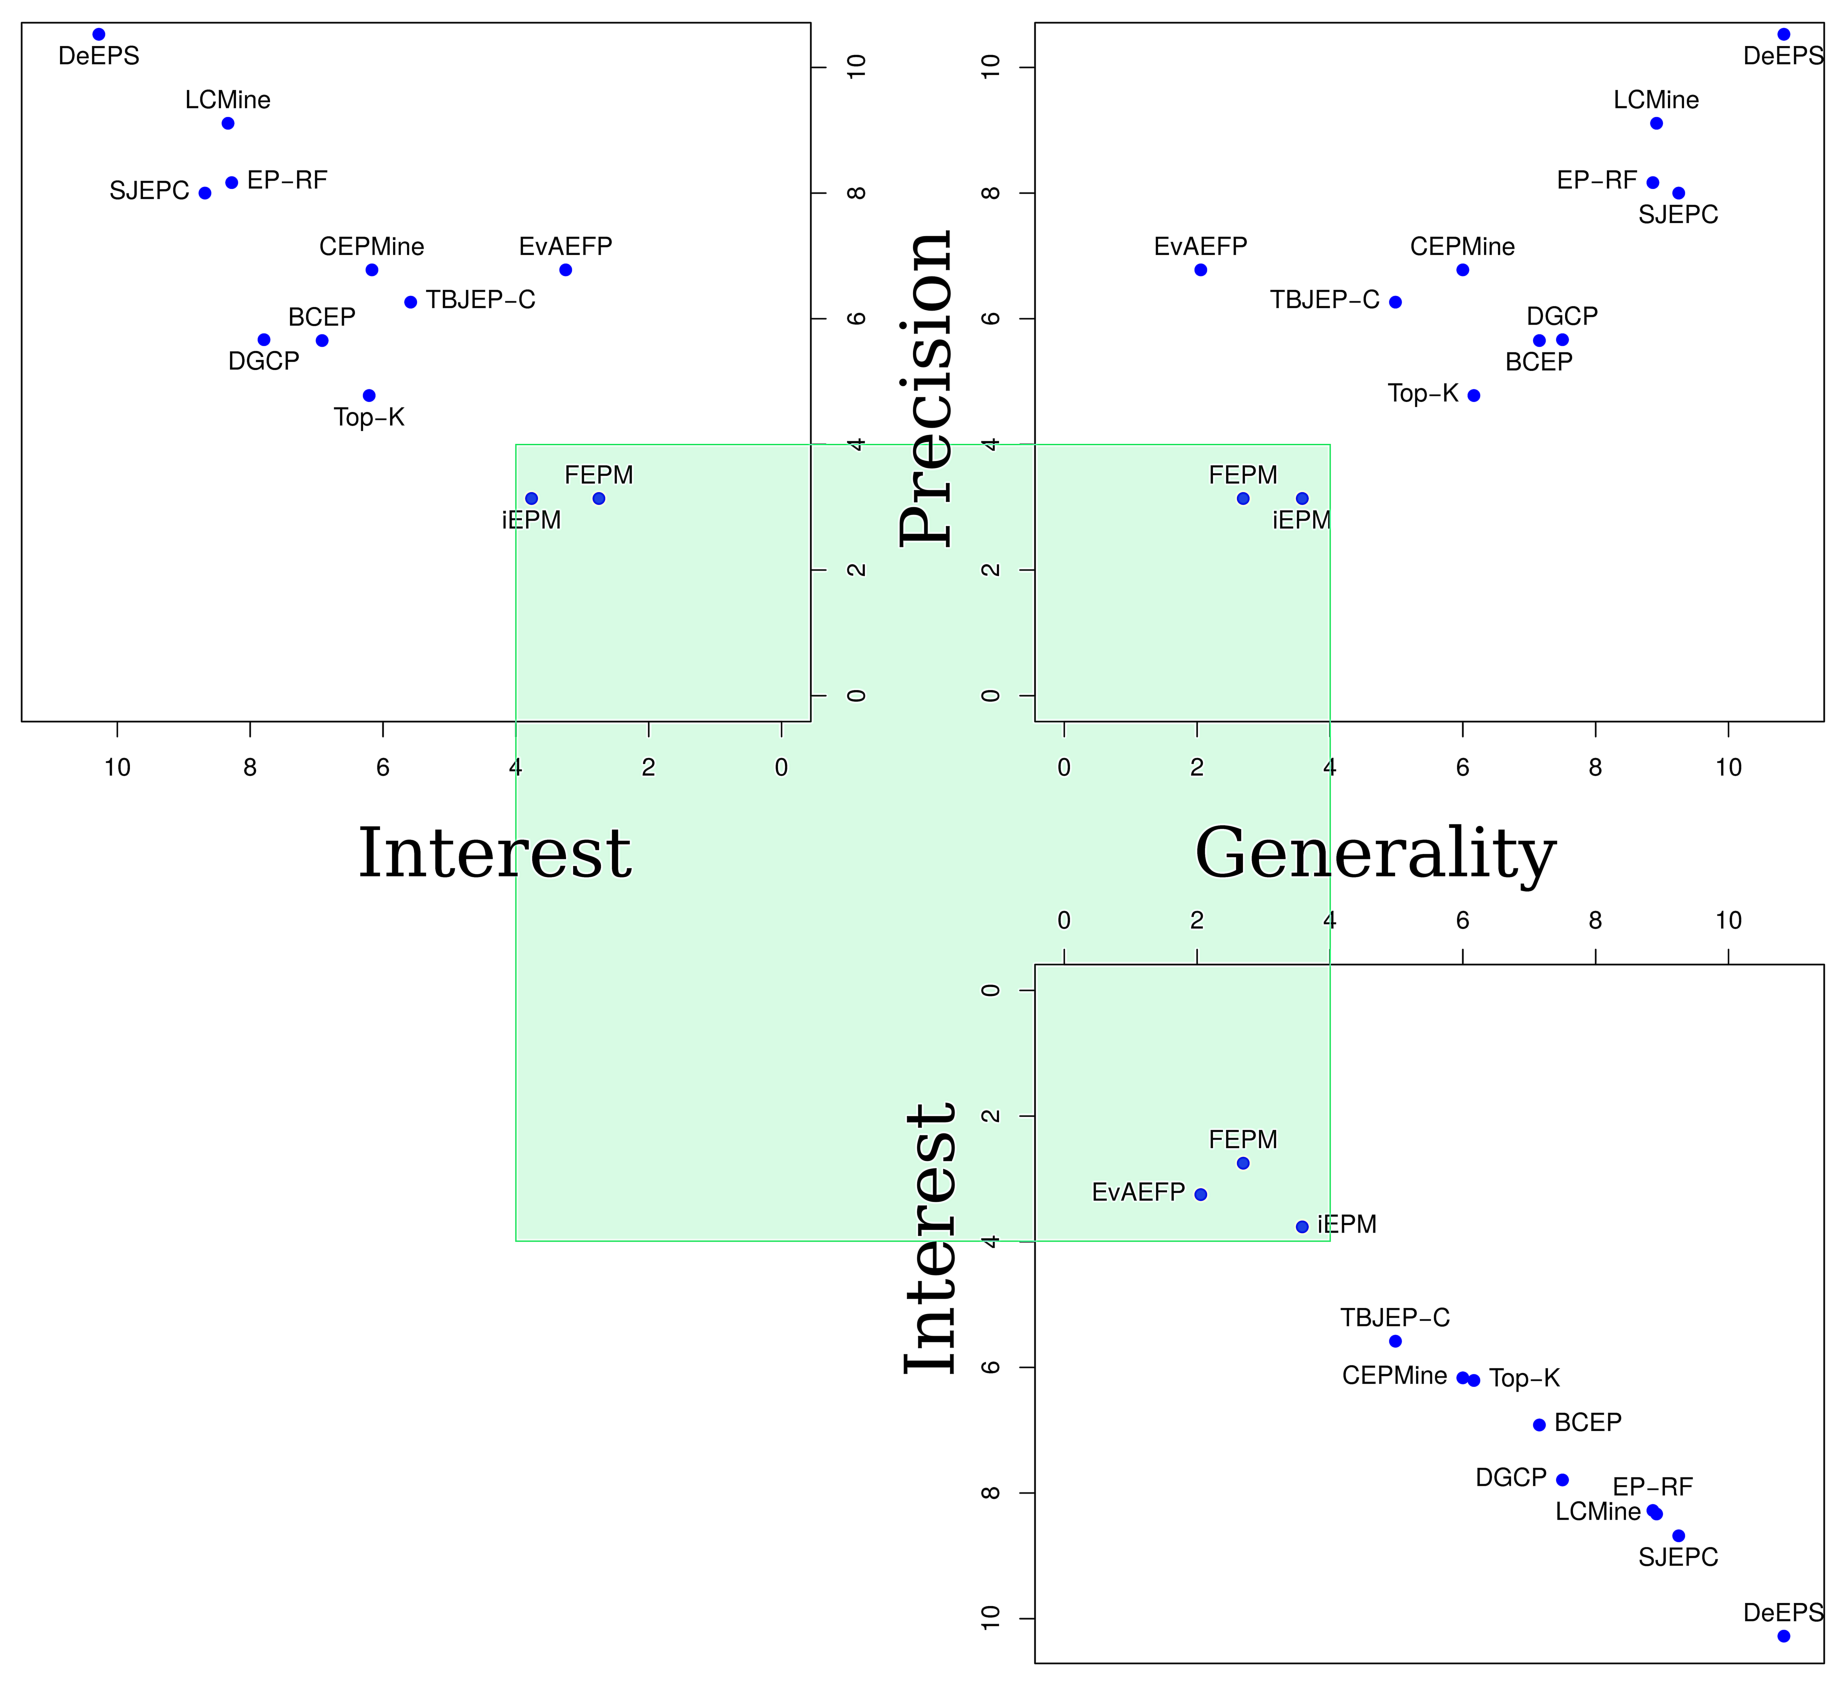
\includegraphics[width=0.7\linewidth]{./Figures/Friedman2.pdf}
		\caption[Comparación del ranking de Friedman de los diferentes algoritmos analizados en el estudio de revisión de EPM.]{Comparación del ranking de Friedman de los diferentes algoritmos analizados en el estudio de revisión de EPM. La zona sombreada en verde indica la zona con mayor relevancia. \textit{Fuente: \cite{Gcmgj18}.}}
		\label{fig:friedman}
	\end{figure}
\end{itemize}

\pagebreak

El trabajo de investigación asociado a esta parte es:

\begin{itemize}
	\item \fullcite{Gcmgj18}. DOI: \doi{10.1002/widm.1231}, IF (JCR 2018): 2.541, Ranking: 26/105 (Computer Science, Theory \& Methods), Cuartil: Q1.
	
	\item \fullcite{Cpggd15}.
	\item \fullcite{Gcgj16}.
	\item \fullcite{Gcd17}.
\end{itemize}


Finalmente, como resultado adicional de la realización de este estudio se ha desarrollado la herramienta de código abierto  EPM-Framework\footnote{\url{https://github.com/SIMIDAT/epm-framework}}, que contiene los algoritmos de \ac{EPM} utilizados en este estudio. El software está en constante desarrollo y tiene como objetivo permitir la aplicación de los principales algoritmos de extracción de patrones emergentes de una forma sencilla e intuitiva, permitiendo la expansión del mismo con nuevas propuestas fácilmente. Se espera que esta herramienta tenga un impacto importante en la comunidad de \ac{EPM}, ampliando la visibilidad y aplicabilidad de estos modelos.

\section{MOEA-EFEP: algoritmo evolutivo multi-objetivo para la extracción de patrones emergentes difusos} \label{sec:moea-efep}

Los resultados obtenidos en el trabajo anterior animan a seguir con el desarrollo de algoritmos basados en sistemas difusos evolutivos para la extracción de patrones emergentes, pues poseen un buen balance entre la fiabilidad de los patrones obtenidos, su generalidad y la interpretabilidad de los modelos. El único algoritmo que hasta la fecha estaba basado en un sistema difuso evolutivo era el algoritmo EvAEP \cite{Gmacd16}, que utiliza un algoritmo evolutivo mono-objetivo. 

La extracción de patrones descriptivos tiene en cuenta tres objetivos fundamentales y que son contrarios entre sí: fiabilidad, generalidad e interpretabilidad. Por lo tanto, un enfoque multi-objetivo resulta adecuado para esta tarea ya que nos permitirá obtener aquellos patrones con mejor balance entre los diferentes objetivos, es decir, los patrones que se encuentren en el frente de Pareto.

En este trabajo se presenta un sistema difuso evolutivo multi-objetivo denominado MOEA-EFEP (\textit{Multi-Objective Evolutionary Algorithm for Extracting Fuzzy Emerging Patterns}) el cual introduce una serie de mecanismos que fomentan la extracción de patrones emergentes descriptivos, apoyándose en las conclusiones extraídas en el trabajo de revisión presentado anteriormente. En concreto, las principales características del método propuesto se presentan a continuación:

\begin{itemize}
	\item Sistema difuso evolutivo basado en ordenación por dominancia \cite{Dapm02}. 
	
	\item Representación ``cromosoma = patrón'' donde un individuo de la población representa un potencial patrón. Se permite además el uso represantación canónica o \ac{DNF} en función de las necesidades del usuario.
	
	\item Esquema cooperativo-competitivo para la extracción del conjunto final de patrones. Se hace uso de una población élite en donde los individuos cooperarán para obtener un conjunto de patrones cuyo valor \ac{WRAcc} medio sea máximo.
	
	\item Dicha población élite se actualiza mediante el operador de \textit{token competition} \cite{Llsy92} si el valor WRAcc medio de la población tras aplicar este operador es mejor que el de la población élite actual. Este operador permite la obtención de aquellos patrones de mayor calidad, cubriendo el mayor espacio de búsqueda posible, evitando la redundancia y reduciendo el solapamiento entre patrones. 
	
	\item Uso de operadores genéticos orientados a impulsar la generalidad de los patrones, como el operador de inicialización basado en patrones generales, una mutación orientada a la generalidad y un operador de reinicialización guiada para moverse a zonas del espacio de búsqueda aún no exploradas.
	
	\item Al finalizar el proceso evolutivo, se emplea un filtro a elegir por parte del usuario entre filtro por confianza, por patrones maximales o patrones minimales, de acuerdo al estudio de revisión presentado anteriormente.
\end{itemize}

El estudio experimental llevado a cabo en este trabajo tiene tres objetivos fundamentales: (1) determinar la mejor representación del conocimiento para el algoritmo propuesto, (2) determinar el tipo de filtro a aplicar tras finalizar el proceso evolutivo, y (3) comparar la calidad de los patrones extraídos frente a los mejores métodos según el estudio de revisión presentado anteriormente. Para ello, los análisis se han realizado utilizando 50 conjuntos de datos, empleando pruebas estadísticas para determinar el nivel de significación de las diferencias.

Las conclusiones que se extraen del estudio experimental llevado a cabo se presentan a continuación:

\begin{itemize}
	\item Existe un mejor balance fiabilidad-generalidad a favor de la representación \ac{DNF} respecto a la representación canónica, con unos niveles de interpretabilidad similares. Esto se puede deber a la mayor flexibilidad que ofrece este tipo de representación al permitir varios valores para una misma variable.
	
	\item La aplicación de un filtro por confianza para el algoritmo propuesto permite la mejora de manera significativa de la fiabilidad de los patrones extraídos, manteniendo los niveles de generalidad e interpretabilidad.
	
	\item Comparado con otros métodos, el algoritmo propuesto es capaz de aumentar el balance generalidad-fiabilidad aumentando de manera significativa la generalidad de los patrones extraídos, mientras que la fiabilidad se mantiene similar con respecto al resto de algoritmos. Además, la interpretabilidad de los patrones extraídos es mejor que el resto al devolver un número muy reducido de reglas. Estos resultados implican una extracción de patrones más interesantes por parte del algoritmo propuesto respecto al resto de métodos analizados.
	
	\item Finalmente, el tiempo de ejecución es de media el más rápido con respecto al resto de métodos, ya que su complejidad depende del número de variables e instancias del problema, mientras que el resto depende del número de selectores e instancias, siendo habitualmente el número de selectores mucho mayor que el de variables.
\end{itemize}

El trabajo de investigación asociado a esta parte es:

\begin{itemize}
	\item \sloppy \fullcite{Gcgd18}. DOI: \doi{10.1109/TFUZZ.2018.2814577}, IF (JCR 2018): 8.759, Ranking: 6/134 (Computer Science, Artificial Intelligence), Cuartil: Q1.
	
	\item \fullcite{Gmacd16}.
\end{itemize}



\section{BD-EFEP: un enfoque big data para la extracción de patrones emergentes difusos} \label{sec:bd-efep}

Uno de los principales problemas de los enfoques de extracción de patrones emergentes es la falta de escalabilidad. Esto es especialmente grave en entornos \textit{big data}. Los sistemas basados en reglas difusas son relevantes para la comunidad ya que poseen robustez frente a problemas de escalabilidad \cite{Fcdh16,Faah17}. De hecho, se han propuesto en la literatura varios desarrollos de sistemas basados en reglas difusas para la extracción de conocimiento en entornos \textit{big data} en diversas áreas de la minería de datos, como clasificación \cite{Rlbh15,Egsb18}, regresión \cite{Rmb16}, preprocesamiento \cite{Prrtbh15}, reglas de asociación \cite{Plv17}, \ac{SD} \cite{Prpgcd16} y una primera aproximación para \ac{EPM} \cite{Ggdc17}.

En este trabajo se presenta un algoritmo para la extracción de patrones emergentes difusos en entornos \textit{big data} denominado BD-EFEP (\textit{Big Data approach for the Extraction of Fuzzy Emerging Patterns}). Este método utiliza un sistema difuso evolutivo multi-objetivo basado en un esquema cooperativo-competitivo que permite obtener una descripción precisa del problema, abarcando la mayor cantidad del espacio de búsqueda posible. Para ello, el algoritmo propuesto se apoya en el empleo de operadores genéticos que fomentan la extracción de este tipo de patrones, como el operador de inicialización y mutación orientada, junto al empleo del operador de \textit{token competition} y un filtro de confianza para mejorar la precisión de los patrones obtenidos.




La principal aportación realizada en este trabajo es el enfoque distribuido basado en MapReduce de la evaluación de los individuos de la población. Este proceso, representado en la \Cref{fig:BDEFEP_MR}, se aplica únicamente en el momento de realizar la evaluación de los individuos de la población. Esto se debe a que el proceso de evaluación es la operación más costosa del algoritmo evolutivo, ya que para cada individuo hay que realizar un recorrido completo del enorme conjunto de datos. Esta evaluación distribuida funciona de la siguiente manera, para cada individuo: en la fase \textit{map}, se calcula la tabla de contingencia relativa a la partición de datos a procesar. Es importante destacar que este proceso se realiza de manera distribuida. Tras su finalización, estas tablas se agrupan en la fase \textit{reduce} sumando sus valores para obtener la tabla de contingencia final de la que se podrán calcular las diferentes medidas de calidad. Con este proceso, el método propuesto es capaz de obtener los mismos resultados independientemente del número de particiones de datos realizadas.

\begin{figure}[!hbtp]
	\centering
	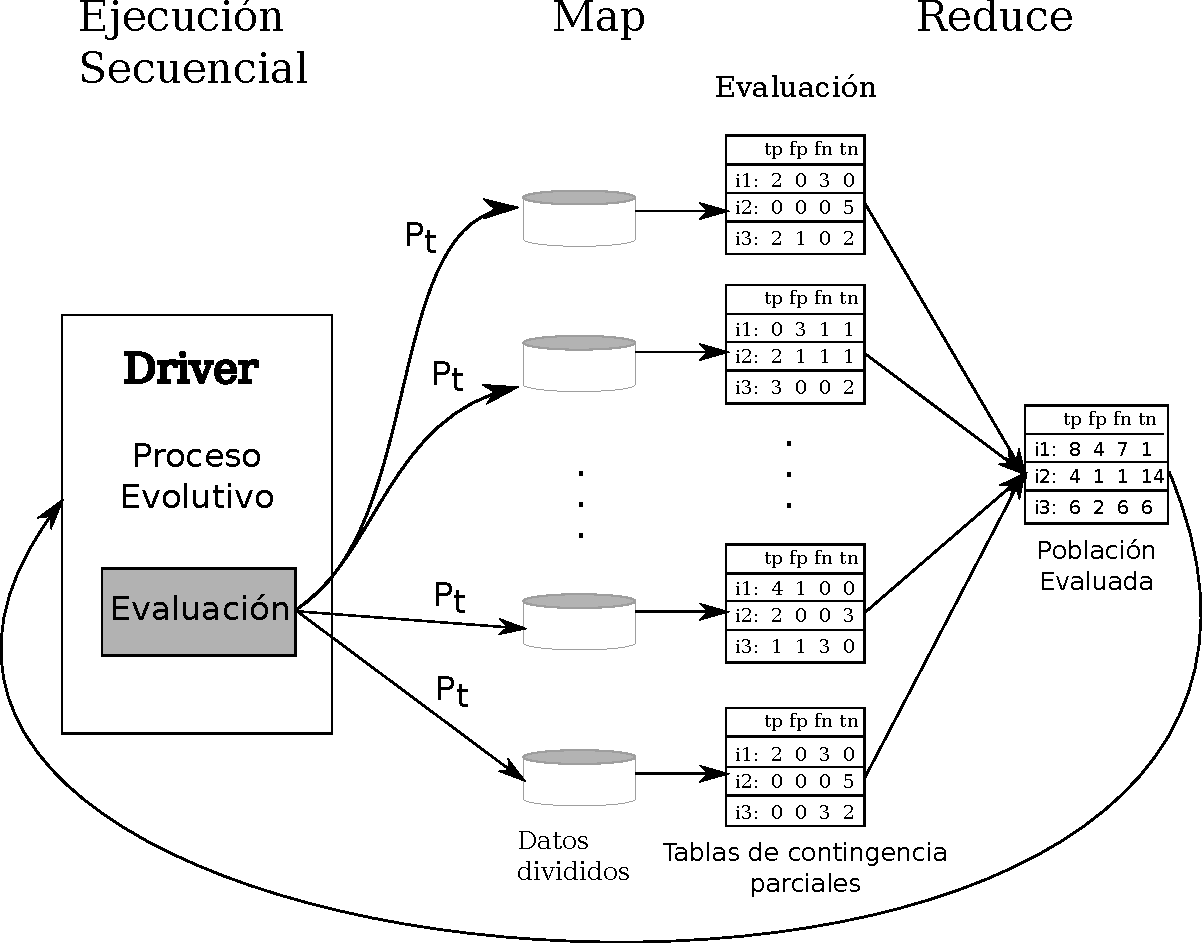
\includegraphics[width=0.7\linewidth]{./Figures/mapReduce_BDEFEP.pdf}
	\caption[Procedimiento de evaluación basado en MapReduce del algoritmo BD-EFEP.]{Procedimiento de evaluación basado en MapReduce del algoritmo BD-EFEP. \textit{Fuente: elaboración propia a partir de \cite{Gcgd19}.}}
	\label{fig:BDEFEP_MR}
\end{figure}

El estudio experimental llevado a cabo tiene dos objetivos: (1) determinar la calidad de los patrones extraídos por BD-EFEP frente a una adaptación para \textit{big data} del algoritmo EvAEP \cite{Gmacd16}, denominada EvAEP-Spark \cite{Ggdc17}; y (2) determinar la escalabilidad de la propuesta respecto a EvAEP-Spark.

Las conclusiones extraídas de este trabajo indican que el algoritmo propuesto obtiene un conjunto de patrones significativamente más preciso que EvAEP-Spark gracias a la aplicación del filtro de confianza final y al empleo de objetivos que promueven la fiabilidad. Sin embargo, la generalidad de estos patrones es peor. A pesar de ello, el balance generalidad-fiabilidad es mejor en BD-EFEP, por lo que los patrones extraídos son más interesantes para el experto. Respecto a la interpretabilidad, gracias al empleo del operador de \textit{token competition} el método extrae bastantes patrones, pero simples. En EvAEP-Spark ocurre el resultado opuesto, se extraen menos patrones, pero más complejos. En este sentido, BD-EFEP mejora la interpretabilidad ya que simplifica de manera significativa el conocimiento obtenido.

Finalmente, la escalabilidad y tiempo de ejecución de BD-EFEP mejora significativamente a EvAEP-Spark. Además, se observa que el método escala de manera adecuada con respecto a la cantidad de particiones realizadas. No obstante, es importante destacar que el tiempo de ejecución para los algoritmos más grandes aún sigue siendo bastante elevado. Por lo tanto, aunque el enfoque MapReduce sea adecuado, estos resultados animan a seguir investigando en el desarrollo de mecanismos y métodos para la ejecución eficiente de algoritmos de extracción de patrones emergentes en entornos \textit{big data}.

El trabajo de investigación asociado a este apartado es:

\begin{itemize}
	\item \fullcite{Gcgd19}. DOI: 10.1007/s12559-018-9612-7, IF (JCR 2018): 4.287, Ranking: 25/134 (Computer Science, Artificial Intelligence), Cuartil: Q1.
	
	\item \fullcite{Ggdc17}.
	\item \fullcite{Ggcd17}.
\end{itemize}








\section{FEPDS: una propuesta para la extracción de patrones emergentes en flujos continuos de datos} \label{sec:streaming}
 
 
Como se ha comentado anteriormente, el tipo de conocimiento extraído en \ac{EPM} es interesante dentro del ámbito de la minería de flujo de datos ya que permite realizar decisiones de manera más sencilla, rápida y fiable. Sin embargo, como se ha visto en el \Cref{sec:ds} la extracción de conocimiento en este ámbito es un reto, debido entre otros, a fuertes restricciones en tiempo de respuesta, uso de memoria y actualización continua del modelo de conocimiento.

En este trabajo se presenta una primera aproximación al problema de extracción de patrones emergentes bajo el paradigma de la minería de flujo de datos, denominado FEPDS (\textit{Fuzzy Emerging Patterns in Data Streams}). Los principales componentes del algoritmo FEPDS se describen a continuación:

\begin{itemize}
	\item Se asume que los datos llegan al método en forma de bloques de datos de tamaño fijo. Para ello, FEPDS implementa un mecanismo que recoge y agrupa dichos datos provenientes del flujo.
	
	\item La adaptación del modelo al estado actual del flujo se lleva a cabo mediante una estrategia de adaptación ciega en donde el modelo se actualiza en cada bloque de datos. Así, se intenta minimizar los efectos de los problemas relacionados con el cambio de concepto  
	
	\item Se emplea una memoria basada en ventana deslizante que almacena los conjuntos de patrones obtenidos recientemente por el algoritmo de aprendizaje. Esta estructura se utilizará para guiar el proceso de búsqueda hacia zonas del espacio que fueron prometedoras recientemente.
	
	\item La principal aportación de este trabajo se encuentra en el algoritmo de aprendizaje de FEPDS, el cual se basa en un sistema difuso evolutivo multi-objetivo basado en ordenación por dominancia cuyas principales características son:
	
	\begin{itemize}
		\item Representación ``cromosoma = patrón'' utilizando un esquema co\-ope\-ra\-ti\-vo-competitivo. La representación se lleva a cabo mediante un vector binario para permitir una representación tipo \ac{DNF} de los patrones, agilizando la aplicación de operadores genéticos gracias al empleo de operaciones de bits.
		
		\item Uso de operadores genéticos orientados a la extracción de patrones con buen balance entre precisión y fiabilidad.
		
		\item Empleo de mecanismos de reinicio en caso de estancamiento para guiar el proceso de búsqueda hacia zonas prometedoras del espacio. Esto se realiza mediante la aplicación del operador de \textit{token competition} usando la información incluida en la memoria basada en ventana deslizante descrita anteriormente.
	\end{itemize}
\end{itemize}

Todos estos componentes se relacionan entre sí para obtener conocimiento de manera continua. El esquema de funcionamiento se encuentra gráficamente representando en la \Cref{fig:fepds}. A modo de resumen, el algoritmo propuesto se basa en: primero, recolectar los datos provenientes del flujo de datos hasta formar un bloque. Dicho bloque se emplea a continuación para evaluar el modelo actual, si existe. Tras esto, se actualiza el modelo de conocimiento actual empleando el algoritmo de aprendizaje junto a los nuevos datos. Finalmente, el conjunto de patrones extraído se añade a la memoria basada en ventana deslizante que se utilizará dentro del proceso de aprendizaje para guiar la búsqueda.

\begin{figure}[!hbtp]
	\centering
	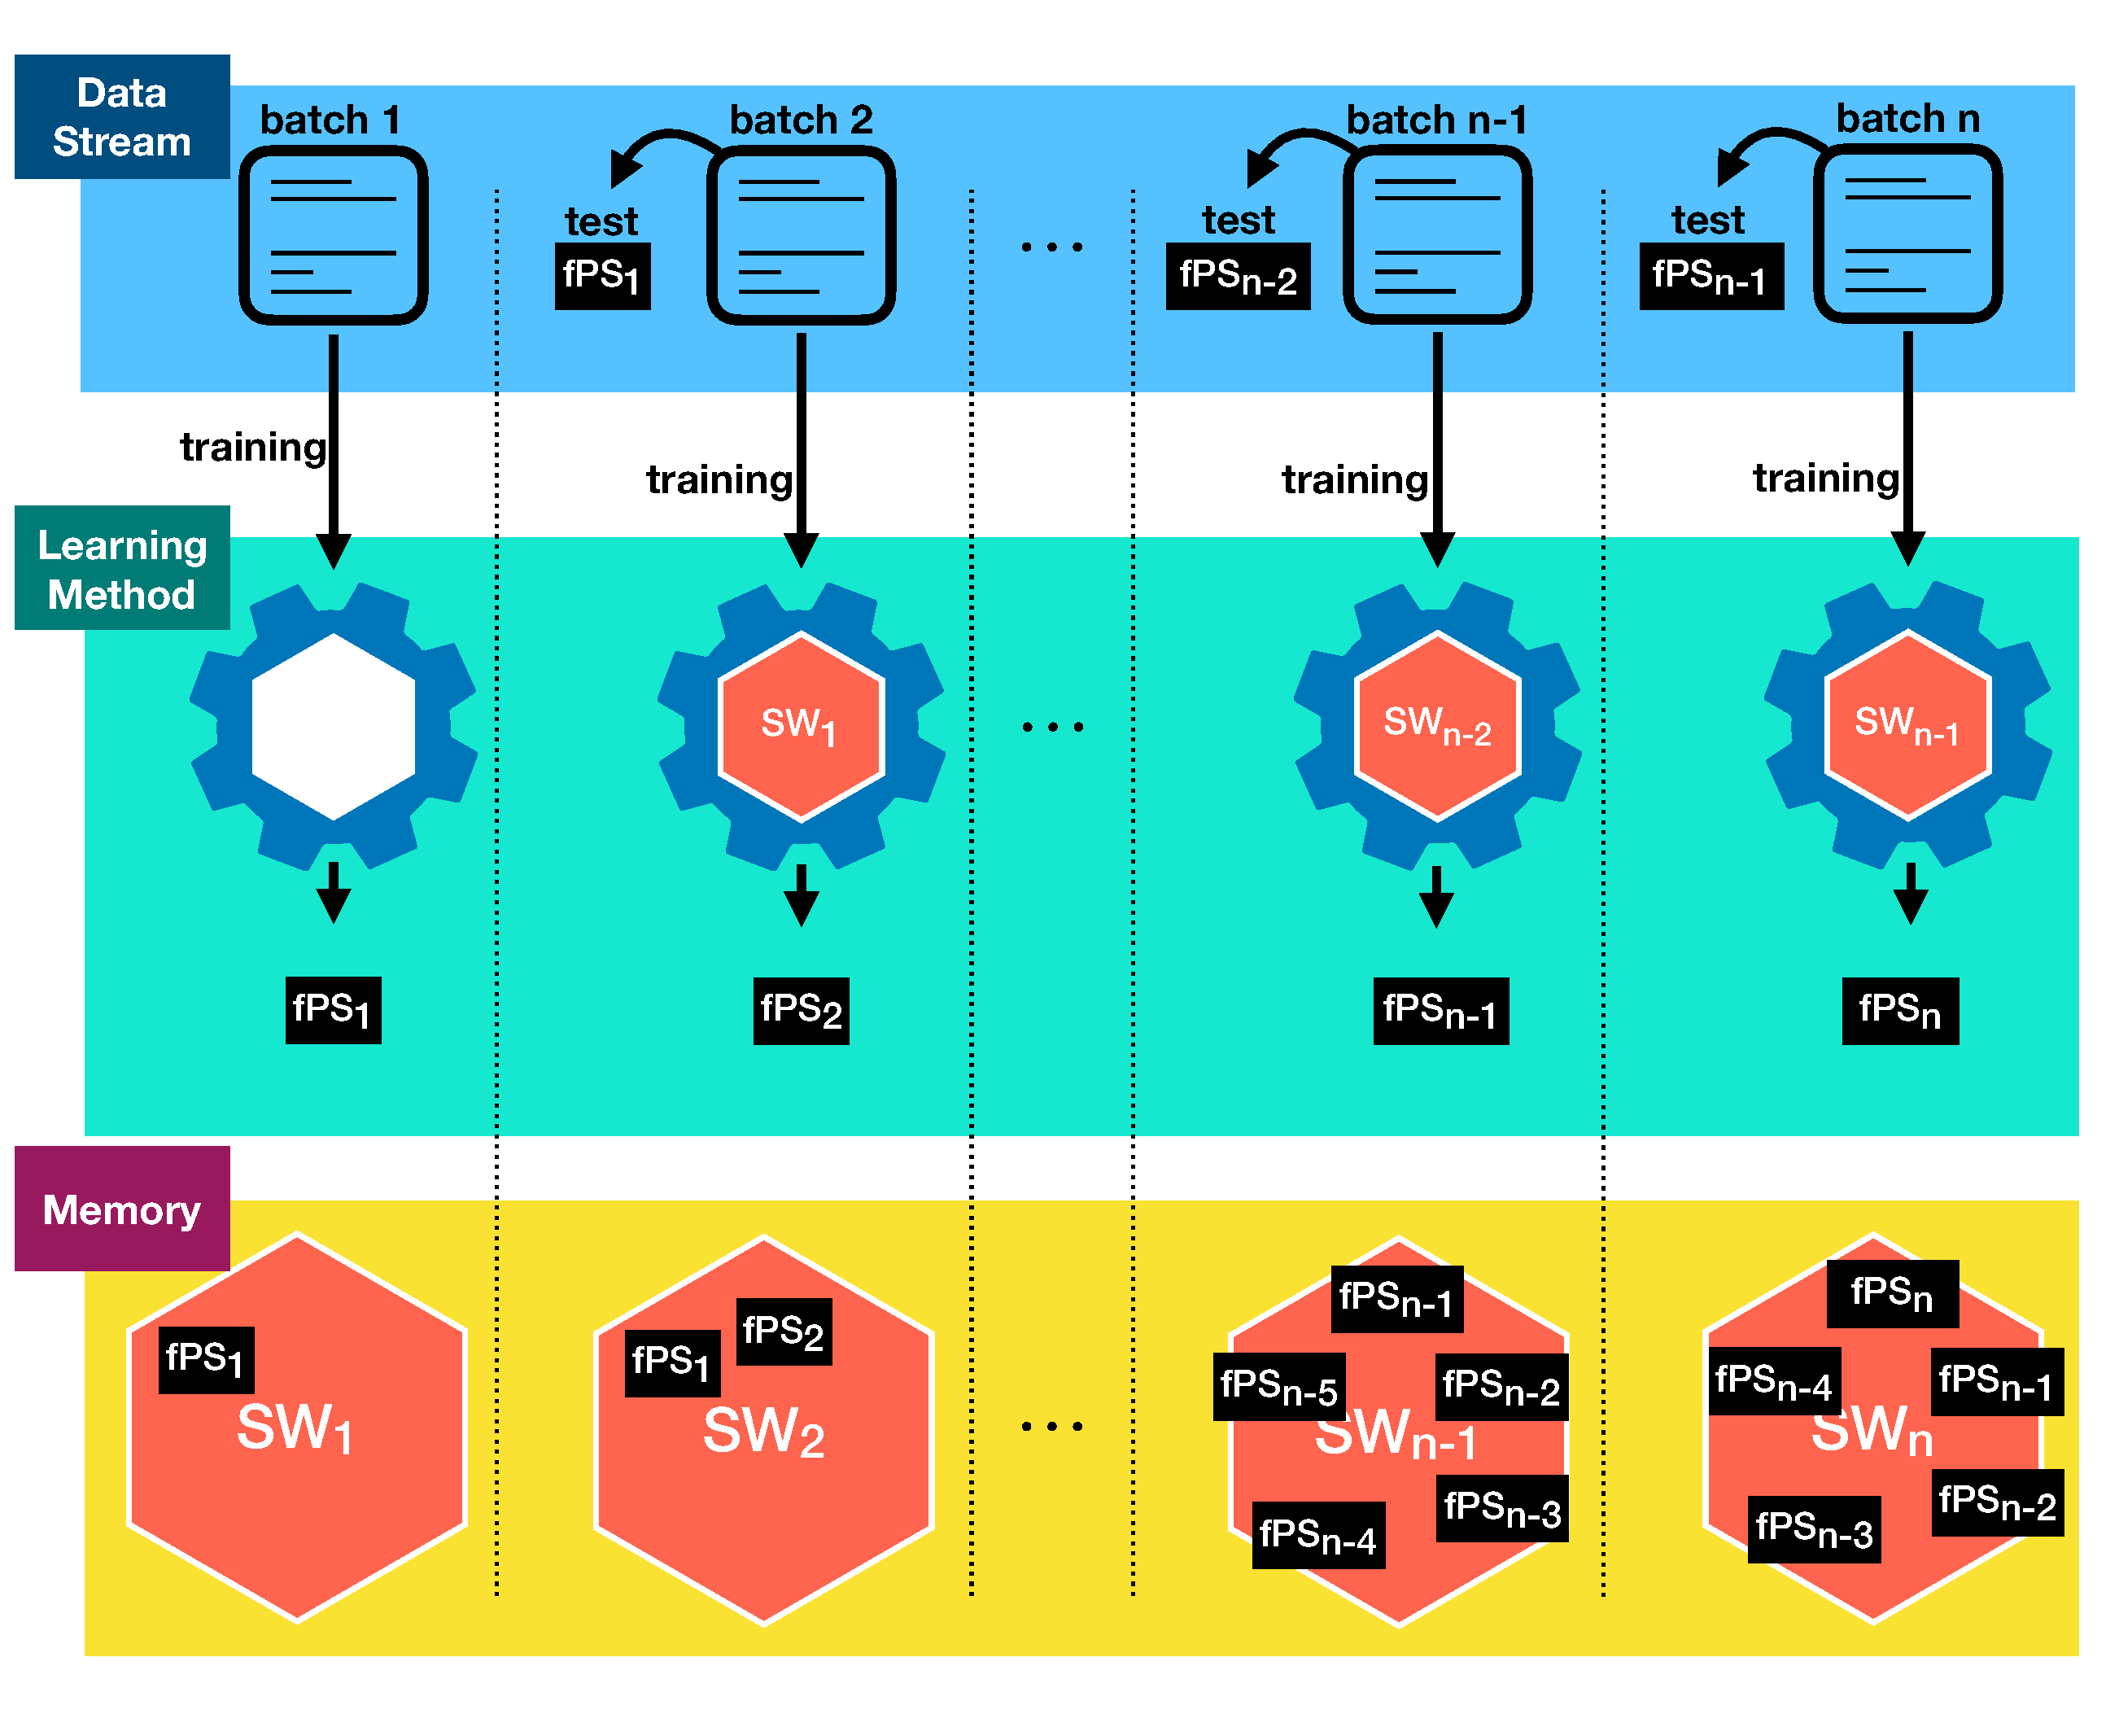
\includegraphics[width=0.7\linewidth]{./Figures/fepds.pdf}
	\caption[Esquema de funcionamiento general del algoritmo FEPDS.]{Esquema de funcionamiento general del algoritmo FEPDS. \textit{Fuente: \cite{Gcgd19a}.}}
	\label{fig:fepds}
\end{figure}

El algoritmo FEPDS ha sido analizado en un amplio estudio experimental con la finalidad de determinar tres objetivos fundamentales: (1) la adaptabilidad del método a posibles cambios de concepto, (2) la calidad media del conocimiento extraído y (3) la escalabilidad y estabilidad del algoritmo a lo largo del tiempo. Finalmente, para demostrar la utilidad real del mismo, se ha llevado a cabo un caso de estudio en donde se describe de manera continua el perfil de los usuarios de los taxis de la ciudad de Nueva York durante el año 2017.

Las conclusiones extraídas del estudio llevado a cabo sugieren que el enfoque de adaptación propuesto, unido al empleo de lógica difusa, permite una gran robustez del sistema frente a cambios de concepto reales. Asimismo, la calidad del conocimiento extraído posee un ratio generalidad-fiabilidad muy interesante para el experto, junto a una interpretabilidad muy buena debido al bajo número de patrones y su simplicidad. Por último, el rendimiento del algoritmo respecto al tiempo de respuesta permite procesar datos a una velocidad aproximada de hasta 5 KHz sin comprometer la estabilidad del sistema, por lo que hace que sea una alternativa viable para el procesamiento de datos en gran cantidad de aplicaciones.

Este hecho se ve reflejado en el caso de estudio abordado en este trabajo. En él, se muestra que la calidad media de los patrones extraídos es muy interesante para los expertos, pudiéndose realizar decisiones a corto plazo de manera sencilla. Además, la capacidad de FEPDS no se limita al corto plazo. Gracias a que es capaz de almacenar el conocimiento extraído, se pueden realizar análisis para decisiones a largo plazo. En concreto, en este estudio se analizan patrones recurrentes para la extracción de un perfil general de usuario a lo largo del año. Por lo tanto, el algoritmo FEPDS es una primera aproximación prometedora que anima a continuar esta línea de investigación en el futuro.

\pagebreak

El trabajo de investigación asociado a esta parte es:

\begin{itemize}
	\item \fullcite{Gcgd19a}. DOI: No disponible, IF (JCR 2018): 8.759, Ranking: 6/134 (Computer Science, Artificial Intelligence), Cuartil: Q1.
	
	\item \fullcite{Gcgd18b}.
\end{itemize}






\clearpage{} \cleardoublepage
\clearpage{}

\chapter{Conclusiones y trabajos futuros} \label{chap:conclusion}

En este capítulo se resumen los resultados obtenidos en los trabajos presentados en esta memoria y se extraen las conclusiones del trabajo realizado. Asimismo, se comentan aspectos relacionados con los trabajos futuros que se pueden realizar siguiendo las líneas de investigación desarrolladas en esta memoria.



Tal y como se ha presentado a lo largo del presente estudio:

\begin{enumerate}

	\item Para la técnica de \ac{SD} existe un amplio abanico de desarrollos a lo largo de la literatura, pero muy pocos están enfocados a problemas complejos. De hecho, hasta donde llega nuestro conocimiento, no existe un método de \ac{SD} enfocado a la extracción de conocimiento en problemas \ac{MIL} ni en entornos de minería de flujo de datos. Para análisis de datos voluminosos, a pesar de existir métodos enfocados a este tipo de datos, no se ha analizado el efecto de factores externos que pueden influir en la calidad de los mismos, como es la presencia de ruido.
	
	\item Las propiedades descriptivas de \ac{EPM} son muy interesantes para el experto, pero el aspecto descriptivo de esta tarea no ha sido impulsado por parte de la literatura especializada. En este sentido, \ac{EPM} se ha utilizado como un medio de clasificación en donde se maximiza la precisión, teniendo muy poco en cuenta el carácter descriptivo.
	
	\item La revisión de la bibliografía del tema muestra que el desarrollo de métodos de minería de patrones emergentes para problemas complejos está muy poco desarrollado.
	
	\item Finalmente, es importante señalar que las técnicas \ac{SDRD} no se encuentran disponibles en los principales software de análisis de datos. En este sentido es interesante incluir este tipo de métodos dentro de estos entornos software para poder proporcionar una respuesta a la necesidad de analizar datos mediante este enfoque.
\end{enumerate}

Para afrontar esta situación, la investigación realizada se centra principalmente en el análisis y desarrollo de soluciones algorítmicas con el objetivo de poder aplicar este tipo de técnicas en problemas complejos. En concreto, la tesis gira en torno a las tareas de \ac{SD} y \ac{EPM} aplicadas a este tipo de problemas.



\section{Conclusiones relacionadas con descubrimiento de subgrupos}

La primera parte de la investigación se orienta a \ac{SD}. Las conclusiones de los trabajos realizados en este área se presentan a continuación:

\begin{itemize}

	
	\item Una de las principales características de los problemas complejos es, entre otras, la diversidad de fuentes de donde provienen los datos. Esta diversidad aumenta la probabilidad de introducir ruido en el sistema, reduciendo su rendimiento. A pesar de que existen varios desarrollos basados en sistemas difusos evolutivos para \ac{SD}, no existe un análisis formal de su robustez en \ac{SD}. Para solucionar esto, se presenta un análisis acerca de la influencia de ruido en este tipo de métodos y la eficacia de aplicar filtros de ruido clásicos, orientados a clasificación, sobre los mismos. Los resultados destacan el funcionamiento de FuGePSD, el cual es capaz de aislar e ignorar el ruido, mientras que en el resto la aplicación de un filtro ayuda a paliar estos efectos negativos. 

	\item Uno de los problemas complejos actualmente en auge son los problemas \ac{MIL}, entre los cuales se encuentran, por ejemplo, problemas de segmentación de imágenes o síntesis de moléculas, entre otros. Este tipo de problemas son especialmente interesantes en \ac{SD}, pero no pueden ser abordados por los enfoques actuales. Por ello, se presenta un estudio con la adaptación a problemas \ac{MIL} de los principales enfoques desarrollados para \ac{SD}. Los resultados muestran que los enfoques clásicos no presentan buena calidad, mientras que los enfoques basados en algoritmos evolutivos permiten obtener una mejor calidad en la mayoría de problemas. Por lo tanto, este trabajo abre una nueva línea de investigación enfocada al desarrollo de métodos \ac{SD} aplicados a problemas \ac{MIL}.
	
	\item Como resultado del estudio realizado de la literatura relacionada con \ac{SDRD} para conocer todo lo realizado y la identificación de problemas abiertos, se analiza una gran cantidad de software específico que contiene los algoritmos más destacados de \ac{SD}. No obstante, la falta de este tipo de paquetes de software en las herramientas de análisis de datos más populares, como R o Python, impide que el alcance de la tarea sea mucho más amplio. Para paliar este déficit, se desarrolla al inicio de esta tesis como resultado de la revisión bibliográfica realizada, el paquete SDEFSR. Este paquete contiene los principales algoritmos de \ac{SD} basados en sistemas difusos evolutivos, así como herramientas específicas de procesamiento básico de patrones, junto a una interfaz web para su manejo. \end{itemize}

En esta parte de la tesis doctoral se ha realizado un profundo trabajo de análisis de diferentes problemas de interés para la comunidad de \ac{SD}. La principal conclusión obtenida es la capacidad de los algoritmos evolutivos en general, y de los sistemas difusos evolutivos en particular, para adaptarse a nuevos entornos y tipos de problemas manteniendo un buen nivel de calidad. De hecho, los trabajos realizados en \ac{SD} abren nuevas líneas de investigación para la mejora de los problemas que se presentan en los mismos.

\section{Conclusiones relacionadas con minería de patrones emergentes}

La segunda parte del desarrollo de esta memoria de tesis está orientada a \ac{EPM}. Las conclusiones extraídas de los trabajos realizados se indican a continuación:

\begin{itemize}
	\item Uno de los primeros objetivos de esta parte es el análisis de los diferentes enfoques desarrollados a lo largo de la literatura para \ac{EPM} desde el punto de vista descriptivo. El resultado de este estudio es una agrupación de los diferentes subconjuntos de patrones emergentes en función de ciertas características interesantes y una taxonomía de algoritmos en función del enfoque que tienen. Además, estos métodos son analizados desde el punto de vista descriptivo. Las conclusiones obtenidas destacan las capacidades descriptivas que presentan los patrones tipo Chi, y el empleo de lógica difusa para mejorar las características descriptivas de los patrones emergentes. Finalmente, el estudio refleja las altas capacidades descriptivas que poseen los enfoques basados en sistemas difusos evolutivos.
	
	\item A continuación, se desarrolla una propuesta para la obtención de sistemas difusos evolutivos que explote todas las características positivas para la extracción de patrones emergentes altamente descriptivos propuestas en el estudio anterior, el algoritmo MOEA-EFEP. Este método se basa en un algoritmo evolutivo multiobjetivo que mediante el empleo de operadores genéticos orientados específicamente a la extracción de patrones simples, y el empleo del operador de \textit{token competition}, fomentan la extracción de patrones emergentes altamente descriptivos. Los resultados obtenidos demuestran un buen balance entre generalidad y fiabilidad de los patrones extraídos, sobrepasando significativamente a los principales enfoques desarrollados en la literatura. Por tanto, el algoritmo MOEA-EFEP es una interesante alternativa para la extracción de conocimiento de calidad para la tarea de \ac{EPM}.
	
	\item Se ha propuesto el algoritmo BD-EFEP, un sistema difuso evolutivo para \ac{EPM} enfocado a abordar problemas \textit{big data}. La principal novedad de este método es el empleo de un procedimiento exacto para la gestión de datos a gran escala gracias a que se distribuye el proceso computacionalmente más costoso a lo largo del algoritmo: la evaluación de los individuos. Así, el método permite la obtención del mismo modelo de conocimiento independientemente de las particiones empleadas. Los resultados obtenidos demuestran por un lado la buena escalabilidad del método y un tiempo de ejecución aceptable. Además, se demuestra que el método obtiene un mejor balance entre generalidad y fiabilidad que otras propuestas. El enfoque propuesto es una alternativa interesante para la extracción de patrones emergentes de gran calidad en entornos \textit{big data} en un tiempo de ejecución aceptable. 

	\item Finalmente, se desarrolla el algoritmo FEPDS, que presenta un compromiso entre las diferentes características y restricciones de la minería de flujo de datos. Este método hace uso de un sistema difuso evolutivo muy eficiente para la extracción continua de patrones emergentes. Para ello, el algoritmo actualiza el modelo mediante un enfoque ciego, donde se añade el conjunto de patrones a la población inicial para ser actualizado, junto al empleo de ventanas deslizantes que permiten guiar la búsqueda a zonas prometedoras basándose en datos históricos. El enfoque propuesto es muy interesante para la extracción de conocimiento en este tipo de entornos, ya que extrae patrones de muy alta calidad, en un tiempo aceptable y tratando adecuadamente el cambio de concepto para evitar perder rendimiento.
\end{itemize}

El trabajo de investigación llevado a cabo para \ac{EPM} en esta tesis ha permitido realizar un profundo avance en el conocimiento relacionado con las capacidades descriptivas de la tarea. Como resultado, se han identificado los tipos de patrones y enfoques de minería más interesantes desde este punto de vista. Además, se ha avanzado en la extracción de este tipo de conocimiento en problemas complejos como \textit{big data} y minería de flujo de datos con resultados muy prometedores. 










\section{Trabajos futuros}

En base al trabajo de investigación realizado en esta tesis, se proponen una serie de trabajos futuros. Estos se basan en la ampliación y mejora de las propuestas presentadas, así como en afrontar cuestiones sin resolver que han surgido durante el desarrollo de la investigación. 


\begin{itemize}
	
	\item Desarrollo de métodos aún más eficientes para \ac{SDRD} en entornos de grandes volúmenes de datos. En este trabajo de investigación se ha presentado una propuesta para abordar el problema de extracción de este tipo de conocimiento en entornos \textit{big data}. No obstante, es interesante seguir profundizando en esta tarea para la obtención de métodos aún más eficientes y con mayor escalabilidad. 

	\item Desarrollo de técnicas para el análisis distribuido de flujo de datos. A día de hoy la cantidad de datos generados continuamente puede ser tan grande que es necesario realizar un procesamiento distribuido de los mismos para cumplir las restricciones de tiempo de ejecución impuestas en este problema. Actualmente ya existen herramientas como Apache Spark Streaming\footnote{\url{https://spark.apache.org/streaming/}} o Apache Flink\footnote{\url{https://flink.apache.org/}}, entre otras, capaces de realizar esta tarea. Sin embargo, aún no se ha desarrollado ninguna técnica de extracción de modelos SDRD en este ámbito.
	
	\item Eliminación de redundancias en modelos \ac{SDRD}. Los patrones obtenidos en \ac{SDRD} deben ser tratados de manera individual, por lo tanto es interesante evitar en la medida de lo posible patrones con alto nivel de solapamiento. Aunque los algoritmos presentados en este trabajo contienen el mecanismo de \textit{token competition} para evitar redundancias, este no es lo suficientemente potente para eliminar patrones con alto nivel de solapamiento. En este sentido, se hace necesario el desarrollo de métodos capaces de eliminar de manera eficaz y eficiente dichos patrones para poder aplicarse en problemas complejos, especialmente en flujos de datos.
	
	\item Desarrollo de modelos \ac{SDRD} enfocados a problemas singulares en aprendizaje automático. En este trabajo de investigación se ha presentado un análisis introductorio del comportamiento de los principales enfoques \ac{SD} en problemas \ac{MIL}. Este resultado anima al desarrollo de nuevos modelos \ac{SDRD} enfocados a este tipo de problema. Asimismo, existe otro tipo de problemas, denominados multi-etiqueta \cite{herrera2016multilabel}, en los que existe más de una clase asignada a cada instancia. Hasta donde alcanza nuestro conocimiento, este tipo de problema aún no se ha analizado desde el punto de vista descriptivo.



	\item Descripción del cambio de concepto. No sólo es interesante la descripción del estado subyacente de los datos. En algunos problemas también es interesante la identificación de los elementos que han producido un cambio. A este concepto se le denomina en la literatura como \textit{change mining} \cite{Boe11} y las técnicas de \ac{EPM} son capaces de realizar esta tarea. Por lo tanto, es una línea de trabajo futuro a tener en cuenta.
	
	\item Mejora en el tratamiento del cambio de concepto. En el trabajo propuesto en esta investigación, únicamente se han tratado cambios de conceptos reales, pues son los que afectan a la calidad del modelo. Sin embargo, también es interesante desde el punto de vista descriptivo el análisis del cambio de concepto virtual, así como otros tipos de cambio como la aparación/desaparición de variables y/o clases. Por lo tanto, existe una amplia línea de trabajo futuro en el desarrollo de técnicas para el tratamiento eficaz y eficiente de los diversos tipos de cambio de concepto dentro de \ac{SDRD}.
	

	
\end{itemize}

\section{Publicaciones relacionadas con la memoria} \label{sec:relacionadas}

Finalmente, en esta sección se presenta una lista de publicaciones derivadas de los resultados presentados en este documento:

\subsection{Revistas internacionales indexadas en JCR}
	
	\begin{itemize}
		\item \fullcite{Lgpc16}. \\DOI: \doi{10.1007/s00500-016-2300-1}, IF (JCR 2016): 2.472, Ranking: 33/105 (Computer Science, Interdisciplinary Applications), Cuartil: Q2.
		
		\item \fullcite{Gcgcd16}. DOI: \doi{10.32614/RJ-2016-048}, IF (JCR 2016): 1.075, Ranking: 55/124 (Statistics \& Probability), Cuartil: Q2.
		
		\item \fullcite{Gcmgj18}. DOI: \doi{10.1002/widm.1231}, IF (JCR 2018): 2.541, Ranking: 26/105 (Computer Science, Theory \& Methods), Cuartil: Q1.
		
		\item \sloppy \fullcite{Gcgd18}.  DOI: \doi{10.1109/TFUZZ.2018.2814577}, IF (JCR 2018): 8.759, Ranking: 6/134 (Computer Science, Artificial Intelligence), Cuartil: Q1.
		
		\item \fullcite{Gcgd19}. DOI: \doi{10.1007/s12559-018-9612-7}, IF (JCR 2018): 4.287, Ranking: 25/134 (Computer Science, Artificial Intelligence), Cuartil: Q1.
		
		\item \fullcite{Lcgjv19}. DOI: \doi{10.2991/ijcis.d.191213.001}, IF (JCR 2018): 2.153, Ranking: 55/106 (Computer Science, Interdisciplinary Applications), Cuartil: Q3.
		
\item \fullcite{Gcgd19a}.   DOI: No disponible, IF (JCR 2018): 8.759, Ranking: 6/134 (Computer Science, Artificial Intelligence), Cuartil: Q1.
		
.
	\end{itemize}

\subsection{Congresos internacionales}
	
	\begin{itemize}
		\item \fullcite{Gmacd16}.
		\item \fullcite{Ggdc17}.
		\item \fullcite{Ggcd17}.
		\item \fullcite{Cggd19}.
	\end{itemize}
	
\subsection{Congresos nacionales}
	
	\begin{itemize}
		\item \fullcite{Cpggd15}.
		\item \fullcite{Gcgcj15}.
		\item \fullcite{604}.
		\item \fullcite{Gcd17}.
		\item \fullcite{Gcgd18b}.
		\item \fullcite{275}. 
		
	     Este trabajo obtuvo el premio al mejor trabajo en II Workshop en Big Data y Análisis de Datos Escalable, XVIII Conferencia de la Asociación Española para la Inteligencia Artificial, Granada, Octubre 2018.
	\end{itemize}

\subsection{Seminarios impartidos}

	\begin{itemize}
	\item \textit{Supervised Descriptive Rule Models for the Extraction of Knowledge in Big Data and Data Streams}. Intelligent Systems Lab, University of Bristol, Bristol (Reino Unido). Noviembre 2018.
	
		\item \textit{Supervised Descriptive Rule Models for the Extraction of Knowledge in Big Data and Data Streams}. School of Computing and Informatics, DeMontfort University, Leicester (Reino Unido). Diciembre 2018.
	\end{itemize}

\subsection{Premios asociados a la tesis}

\begin{itemize}
	
	\item Mejor trabajo de iniciación a la investigación en IV Premios Ada Lovelace de la Universidad de Jaén. Septiembre 2018.
		
	\item Premio al mejor trabajo en II Workshop en Big Data y Análisis de Datos Escalable, XVIII Conferencia de la Asociación Española para la Inteligencia Artificial, Granada, Octubre 2018.
	
	\item Mejor trabajo de investigación en V Jornadas Doctorales en TIC de la Universidad de Jaén. Mayo 2019.
\end{itemize}

\clearpage{} \cleardoublepage

\begin{otherlanguage}{british}
	\rhead[\footnotesize{\sc{Chapter \thechapter: \rm\leftmark}}]{}   \lhead[ ]{\footnotesize{\sc{\thesection: \rm\rightmark}}}  \clearpage{}\setcounter{chapter}{2}
\chapter{Concluding remarks} \label{chap:conclusion_en}

This chapter summarises the results presented in this thesis and draws conclusions from the work carried out. It also comments on the aspects related to future work that can be carried out along the research lines developed here. As presented throughout this study:


\begin{enumerate}
	\item For the \ac{SD} technique there is a wide range of developments throughout the literature, but very few are focused on complex problems. In fact, to the best of our knowledge, there is no \ac{SD} method focused on extracting knowledge from MIL problems or data stream mining environments. Despite the existence of methods focused on big data, the effect of external factors that can influence the quality of the data, such as the presence of noise, has not yet been analysed.
	
	\item The descriptive properties of \ac{EPM} are very interesting for the expert, but the descriptive aspect of this task has not been driven by the specialized literature. In this way, \ac{EPM} has been used as a means of classification where accuracy is maximised, with little regard for the descriptive capacity.
	
	\item To the best of our knowledge, the development of \ac{EPM} methods for complex problems is still very limited.
	
	\item Finally, it is important to remark that the \ac{SDRD} techniques are not available in the main data analysis software. In this sense it is interesting to include these kinds of methods within this software in order to provide an answer to the need for data analysis through this approach.
\end{enumerate}

To alleviate this situation the research carried out focuses mainly on the analysis and development of algorithmic solutions with the aim of being able to apply this type of technique to complex problems. Specifically, the thesis focuses on the tasks of \ac{SD} and \ac{EPM} applied to this type of problem.


\section{Conclusions related to subgroup discovery}

The first part of the investigation is geared towards \ac{SD}. The conclusions of the work carried out in this area are presented below:

\begin{itemize}
	\item One of the main characteristics of complex problems is the diversity of sources from which the data come. This increases the probability of introducing noise into the system, reducing its performance. Although there are several developments based on evolutionary fuzzy systems for \ac{SD}, there is no formal analysis of their robustness. In order to resolve this, an initial analysis is presented of the influence of noise on these types of methods and the effectiveness of applying classical, classification-oriented noise filters on them. The results highlight the FuGePSD algorithm, which is able to isolate and ignore noise. With respect to the remaining methods, the application of a filter helps to alleviate these negative effects. 
	
	\item Some of the complex problems currently on the rise are \ac{MIL} problems such as image segmentation and molecule synthesis, among others. These types of problems are interesting in \ac{SD}, but cannot be addressed using current approaches. Therefore, a study is presented with the adaptation to \ac{MIL} problems of the main approaches developed for \ac{SD}, based on the \ac{MIL} standard assumption. The results show that the classical approaches do not present good quality results, while those approaches based on evolutionary algorithms allow us to obtain better results for most problems. Therefore, this study opens up a new line of research focused on the development of \ac{SD} methods applied to \ac{MIL} problems.
	
	\item As a result of the in-depth study carried out on the literature related to SDRD, a large amount of specific software containing the most outstanding SDRD algorithms is analysed. However, the lack of such software packages in the most popular data analysis tools, such as R or Python, prevents the scope of the task from being much wider. In order to alleviate this deficit, the SDEFSR package is developed of the bibliographic review carried out. This package contains the main evolutionary fuzzy system-based algorithms, as well as specific basic pattern processing tools, along with a web interface for easy use. The response of the community to this package has been acceptable and encourages the continuous improvement of the package to expand its influence.
\end{itemize}

In this part of the doctoral thesis, an in-depth analysis of different problems that are of interest to the \ac{SD} community has been carried out. The main conclusion obtained is the capacity of evolutionary algorithms in general, and evolutionary fuzzy systems in particular, to adapt to new environments and types of problems while maintaining a good level of quality. In fact, the work carried out opens up new research lines for the improvement of the problems presented in them.

\section{Conclusions related to emerging pattern mining}

The second part of the development of this thesis is oriented towards \ac{EPM}. The conclusions drawn from the work carried out are set out below:

\begin{itemize}
	\item One of the first objectives of this part is an analysis of the different approaches developed throughout the literature for \ac{EPM} from a descriptive point of view. The result of this study is a grouping of the different subsets of emerging patterns according to certain interesting characteristics, together with an algorithmic taxonomy depending on the approach taken. In addition, these methods are analysed from a descriptive point of view. The conclusions obtained highlight the descriptive capabilities of Chi-type patterns and the use of fuzzy logic to improve the descriptive characteristics of the emerging patterns. Finally, the study reflects the high descriptive capabilities of evolutionary fuzzy system approaches.
	
	\item Next, an evolutionary fuzzy system is developed in order to exploit all the positive features for the extraction of highly descriptive emergent patterns proposed in the previous study, the MOEA-EFEP algorithm. This method is based on a multi-objective evolutionary algorithm. It uses genetic operators specifically oriented to the extraction of simple patterns together with the use of the token competition operator, which encourages the extraction of highly descriptive emerging patterns. The results obtained show a good balance between generality and reliability of the extracted patterns, significantly surpassing the main approaches developed in the literature. Therefore, we conclude that the MOEA-EFEP algorithm is an interesting alternative for the extraction of quality knowledge for the \ac{EPM} task.
	
	\item The BD-EFEP algorithm, an evolutionary fuzzy system for \ac{EPM} focused on addressing big data problems, has been proposed. The main novelty of this method is the use of an exact procedure for large-scale data management because only the most computationally expensive process is distributed throughout the algorithm: the evaluation of individuals. Thus, the method allows the extraction of the same knowledge model regardless of the partitions used. The results obtained demonstrate the good scalability of the method and an acceptable execution time. Furthermore, it is shown that the method achieves a better balance between generality and reliability than other proposals. The conclusion drawn from this work is that the proposed approach is an interesting alternative for the extraction of high quality emerging patterns in big data environments at an acceptable execution time. 
	
	\item Finally, the FEPDS algorithm is developed, which presents a compromise between the different characteristics and constraints of data stream mining. This method uses a very efficient evolutionary fuzzy system for the continuous extraction of emerging patterns. In order to do this the algorithm updates the model using a blind approach, where the set of patterns is added to the initial population to be updated together with the use of sliding windows that allow the search to be guided to promising areas based on historical data. The conclusion obtained from this work suggests that the proposed approach is very interesting for knowledge extraction in this type of environment. The method is able to extract very high quality patterns, in an acceptable execution time, while the concept drift is handled adequately.
\end{itemize}

The research work carried out in this thesis has allowed an advance in knowledge related to the descriptive capacities of the \ac{EPM} task. As a result, the most interesting types of patterns and mining approaches have been identified from this point of view. In addition, progress has been made in extracting this type of knowledge in complex problems such as big data and data stream mining with very promising results. 







\section{Future work}

Based on the research work carried out in this thesis a series of future studies are proposed. These are mainly based on extending and improving the presented proposals, as well as addressing unresolved issues that have arisen during the development of the research. 


\begin{itemize}
	
	\item Development of efficient methods for \ac{SDRD} in big data environments. In this study, a proposal has been presented to address the problem of extracting this type of knowledge in big data environments. However, it is interesting to continue the research on this task in order to obtain even more efficient and scalable methods. 
	
	\item Development of techniques for distributed data stream analysis. Today the amount of data generated can be so large that distributed processing of the data is necessary to meet the runtime restrictions imposed on this problem. Currently, there are tools such as Apache Spark Streaming\footnote{\url{https://spark.apache.org/streaming/}} and Apache Flink\footnote{\url{https://flink.apache.org/}}, among others, capable of performing this task. However, no \ac{SDRD} model extraction technique has been developed in this area yet.
			
	\item Elimination of redundancies in \ac{SDRD} models. The patterns obtained in \ac{SDRD} must be treated individually, so it is interesting to avoid as much as possible redundant or highly overlapping patterns. Although the algorithms presented in this study contain the mechanism of token competition in order to avoid redundancies, this is not powerful enough to eliminate patterns with a high level of overlap. In this way, it is necessary to develop methods capable of effectively and efficiently removing such patterns so that they can be applied to complex problems, especially in data streams.
			
	\item Development of models focused on new complex problems. In this study, an introductory analysis of the behaviour of the main \ac{SD} approaches in \ac{MIL} problems has been presented. This result encourages the development of new models focused on this type of problem. There is also another type of complex problem, called multi-label \cite{herrera2016multilabel}, when there is more than one class assigned to each instance. To the best of our knowledge, this type of problem has not been analysed from the \ac{SDRD} point of view yet.
			


	
			
	\item Description of the concept drift. Not only the description of the underlying state of the data is interesting. In some problems it is also interesting to identify the elements that have produced a change. This concept is referred to in the literature as \textit{change mining} \cite{Boe11} and \ac{EPM} techniques are capable of performing this task. Therefore, it is future work to be considered.
			
	\item Improvement in the treatment of concept drift. In the work proposed in this research, only real drifts have been dealt with, as these affect the quality of the model. However, it is also interesting from a descriptive point of view to analyse the virtual drift, as well as other types of change such as the appearance/disappearance of variables and/or classes, amongst others. Therefore, there is a broad future research line in developing techniques for the effective and efficient treatment of various types of concept drifts in this area.
			
		\end{itemize}
		
\section{Associated publications} \label{sec:relacionadas2}
		
		Finally, this section presents a list of publications derived from the results presented in this document:
		
\subsection{International journals indexed in JCR}
		
		\begin{itemize}
		\item \fullcite{Lgpc16}. \\ DOI: \doi{10.1007/s00500-016-2300-1}, IF (JCR 2016): 2.472, Ranking: 33/105 (Computer Science, Interdisciplinary Applications), Quartile: Q2.

\item \fullcite{Gcgcd16}. DOI: \doi{10.32614/RJ-2016-048}, IF (JCR 2016): 1.075, Ranking: 55/124 (Statistics \& Probability), Quartile: Q2.

\item \fullcite{Gcmgj18}. DOI: \doi{10.1002/widm.1231}, IF (JCR 2018): 2.541, Ranking: 26/105 (Computer Science, Theory \& Methods), Quartile: Q1.

\item \fullcite{Gcgd18}.  DOI: \doi{10.1109/TFUZZ.2018.2814577}, IF (JCR 2018): 8.759, Ranking: 6/134 (Computer Science, Artificial Intelligence), Quartile: Q1.

\item \fullcite{Gcgd19}. DOI: \doi{10.1007/s12559-018-9612-7}, IF (JCR 2018): 4.287, Ranking: 25/134 (Computer Science, Artificial Intelligence), Quartile: Q1.

\item \fullcite{Lcgjv19}. DOI: \doi{10.2991/ijcis.d.191213.001}, IF (JCR 2018): 2.153, Ranking: 55/106 (Computer Science, Interdisciplinary Applications), Quartile: Q3.

\item \fullcite{Gcgd19a}.   DOI: Not available, IF (JCR 2018): 8.759, Ranking: 6/134 (Computer Science, Artificial Intelligence), Quartile: Q1.

.
		\end{itemize}
		
\subsection{International congresses}
		
	\begin{itemize}
	\item \fullcite{Gmacd16}.
	\item \fullcite{Ggdc17}.
	\item \fullcite{Ggcd17}.
	\item \fullcite{Cggd19}.
\end{itemize}
		
\subsection{National congresses}
		
		\begin{itemize}
			\item \fullcite{Cpggd15}.
	\item \fullcite{Gcgcj15}.
	\item \fullcite{604}.
	\item \fullcite{Gcd17}.
	\item \fullcite{Gcgd18b}.
	\item \fullcite{275}. 
	
			This study won the prize for the best paper at the II Workshop on Big Data and Scalable Data Analysis, XVIII Conference of the Spanish Association for Artificial Intelligence, Granada, October 2018.
		\end{itemize}
		
\subsection{Seminars delivered}
		
		\begin{itemize}
			\item \textit{Supervised Descriptive Rule Models for the Extraction of Knowledge in Big Data and Data Streams}. Intelligent Systems Lab, University of Bristol, Bristol (Reino Unido). Noviembre 2018.
			
			\item \textit{Supervised Descriptive Rule Models for the Extraction of Knowledge in Big Data and Data Streams}. School of Computing and Informatics, DeMontfort University, Leicester (Reino Unido). Diciembre 2018.
		\end{itemize}
		
\subsection{Awards received}
		
		\begin{itemize}
			
			\item Best initiation to research work in the 4th Ada Lovelace Awards of the University of Jaén. September 2018.
			
			\item Award to the best work in 2nd Workshop on Big Data and Scalable Data Analysis, 18th Conference of the Spanish Association for Artificial Intelligence, Granada, October 2018.
			
			\item Best research paper at the 5th PhD Conference on Information and Communication Technologies at the University of Jaén. May 2019.
		\end{itemize}\clearpage{} \cleardoublepage
\end{otherlanguage}

\renewcommand{\figurename}{Figura}
\renewcommand{\tablename}{Tabla}

\rhead[\footnotesize{\sc{Cap\'itulo \thechapter: \rm\leftmark}}]{}   \lhead[ ]{\footnotesize{\sc{\thesection: \rm\rightmark}}}  

\clearpage{}








\chapter{Publicaciones indexadas en JCR asociadas}\label{chap:publications}



En virtud con lo establecido en el artículo 25, punto 2, de la normativa vigente de los Estudios de Doctorado de la Universidad de Jaén, correspondiente al programa establecido en el RD. 99/2011, en este capítulo se presenta una colección de trabajos publicados por el doctorando durante su pertenencia al programa de doctorado. Estas publicaciones constituyen el núcleo de la tesis doctoral.

Dichas publicaciones se corresponden con siete artículos científicos publicados en revistas internacionales indexadas en \ac{JCR}. Para cada una de las publicaciones presentadas, se muestra información básica sobre la publicación, así como los principales índices de calidad de las revistas en donde se han publicado los trabajos. Los trabajos mostrados en esta sección son los siguientes:

\begin{itemize}
		\item \fullcite{Lgpc16}. \\DOI: \doi{10.1007/s00500-016-2300-1}, IF (JCR 2016): 2.472, Ranking: 33/105 (Computer Science, Interdisciplinary Applications), Cuartil: Q2.

\item \fullcite{Gcgcd16}. DOI: \doi{10.32614/RJ-2016-048}, IF (JCR 2016): 1.075, Ranking: 55/124 (Statistics \& Probability), Cuartil: Q2.

\item \fullcite{Gcmgj18}. DOI: \doi{10.1002/widm.1231}, IF (JCR 2018): 2.541, Ranking: 26/105 (Computer Science, Theory \& Methods), Cuartil: Q1.

\item \sloppy \fullcite{Gcgd18}.  DOI: \doi{10.1109/TFUZZ.2018.2814577}, IF (JCR 2018): 8.759, Ranking: 6/134 (Computer Science, Artificial Intelligence), Cuartil: Q1.

\item \fullcite{Gcgd19}. DOI: \doi{10.1007/s12559-018-9612-7}, IF (JCR 2018): 4.287, Ranking: 25/134 (Computer Science, Artificial Intelligence), Cuartil: Q1.

\item \fullcite{Lcgjv19}. DOI: \doi{10.2991/ijcis.d.191213.001}, IF (JCR 2018): 2.153, Ranking: 55/106 (Computer Science, Interdisciplinary Applications), Cuartil: Q3.

\item \fullcite{Gcgd19a}.   DOI: No disponible, IF (JCR 2018): 8.759, Ranking: 6/134 (Computer Science, Artificial Intelligence), Cuartil: Q1.
\end{itemize}

\clearpage








\section{\citetitle{Lgpc16}}

\begin{itemize}
	\item  \fullcite{Lgpc16}.
	
	\begin{itemize}
		\item Estado: \textbf{Publicado}.
		\item ISSN: 1432-7643.
		\item DOI: \doi{10.1007/s00500-016-2300-1}.
		\item Factor de Impacto (JCR 2016): \textbf{2.472}.
		\item Categoría: \textbf{Computer Science, Interdisciplinary Applications}.
		\item Ranking: \textbf{33/105}.
		\item Cuartil: \textbf{Q2}.
	\end{itemize}
\end{itemize}


\incluirPaper{3-}{./Papers/2016-Luengo-NoiseSD}


\section{\citetitle{Gcgcd16}}

\begin{itemize}
	\item \fullcite{Gcgcd16}.
	
	\begin{itemize}
		\item Estado: \textbf{Publicado}.
		\item ISSN: 2073-4859.
		\item DOI: \doi{10.1007/s00500-016-2300-1}.
		\item Factor de Impacto (JCR 2016): \textbf{1.075}.
		\item Categoría: \textbf{Statistics \& Probability}.
		\item Ranking: \textbf{55/124}.
		\item Cuartil: \textbf{Q2}.
	\end{itemize}
\end{itemize}


\incluirPaper{-}{./Papers/2016-Garcia-RJournal}





\section{\citetitle{Lcgjv19}}

\begin{itemize}
	\item \fullcite{Lcgjv19}.
	
	\begin{itemize}
		\item Estado: \textbf{Publicado}.
		\item ISSN: 1875-6891.
		\item DOI: \doi{10.2991/ijcis.d.191213.001}.
		\item Factor de Impacto (JCR 2018): \textbf{2.153}.
		\item Categoría: \textbf{Computer Science, Interdisciplinary Applications}.
		\item Ranking: \textbf{55/106}.
		\item Cuartil: \textbf{Q3}.
	\end{itemize}
\end{itemize}

\incluirPaper{-}{./Papers/2019_Luna_MIL}




\section{\citetitle{Gcmgj18}}

\begin{itemize}
	\item \fullcite{Gcmgj18}.
	
	\begin{itemize}
		\item Estado: \textbf{Publicado}.
		\item ISSN: 1942-4795.
		\item DOI: \doi{10.1002/widm.1231}.
		\item Factor de Impacto (JCR 2018): \textbf{2.541}.
		\item Categoría: \textbf{Computer Science, Theory \& Methods}.
		\item Ranking: \textbf{26/105}.
		\item Cuartil: \textbf{Q1}.
	\end{itemize}
\end{itemize}

\incluirPaper{-}{./Papers/2018-Garcia-Wiley}





\section{\citetitle{Gcgd18}}

\begin{itemize}
	\item \sloppy \fullcite{Gcgd18}.
	
	\begin{itemize}
		\item Estado: \textbf{Publicado}.
		\item ISSN: 1063-6706.
		\item DOI: \doi{10.1109/TFUZZ.2018.2814577}.
		\item Factor de Impacto (JCR 2018): \textbf{8.759}.
		\item Categoría: \textbf{Computer Science, Artificial Intelligence}.
		\item Ranking: \textbf{6/134}.
		\item Cuartil: \textbf{Q1}.
	\end{itemize}
\end{itemize}

\incluirPaper{-}{./Papers/2018-Garcia-IEEE_TFS}








\section{\citetitle{Gcgd19}}

\begin{itemize}
	\item \fullcite{Gcgd19}.
	
	\begin{itemize}
		\item Estado: \textbf{Publicado}.
		\item ISSN: 1866-9956.
		\item DOI: \doi{10.1007/s12559-018-9612-7}.
		\item Factor de Impacto (JCR 2018): \textbf{4.287}.
		\item Categoría: \textbf{Computer Science, Artificial Intelligence}.
		\item Ranking: \textbf{25/134}.
		\item Cuartil: \textbf{Q1}.
	\end{itemize}
\end{itemize}

\incluirPaper{-}{./Papers/2019_Garcia_Cognitive}












\section{\citetitle{Gcgd19a}}

\begin{itemize}
	\item \fullcite{Gcgd19a}.
	
	\begin{itemize}
		\item Estado: \textbf{Sometido en segunda vuelta con \textit{major revision}}.
	    \item ISSN: 1063-6706.
		\item DOI: No disponible.
		\item Factor de Impacto (JCR 2018): \textbf{8.759}.
		\item Categoría: \textbf{Computer Science, Artificial Intelligence}.
		\item Ranking: \textbf{6/134}.
		\item Cuartil: \textbf{Q1}.
	\end{itemize}
\end{itemize}

\incluirPaper{-}{./Papers/2019_Garcia_SparkStreaming}
\clearpage{} \cleardoublepage




\backmatter
\rhead[\footnotesize{\sc{Bibliografía}}]{}   \lhead[ ]{\footnotesize{\sc{Bibliografía}}}  \addcontentsline{toc}{chapter}{Bibliografía}
\sloppy
\printbibliography




\end{document}